 %\pdfoutput=1
%\documentclass[conference]{IEEEtran}
\documentclass[lettersize,journal]{IEEEtran}
\normalsize
\IEEEoverridecommandlockouts
% The preceding line is only needed to identify funding in the first footnote. If that is unneeded, please comment it out.
\usepackage{setspace}
\usepackage{array,tabulary,tabularx,multirow}
\usepackage[T1]{fontenc}
\usepackage{cite}
\usepackage{caption}
\captionsetup{font=footnotesize}
\usepackage{algcompatible}
%\usepackage{subcaption}
\usepackage{mathtools}
\usepackage{stackengine}
%\usepackage[caption=false,font=normalsize,labelfont=sf,textfont=sf]{subfig}
\def\delequal{\mathrel{\ensurestackMath{\stackon[1pt]{=}{\scriptstyle\Delta}}}}
\usepackage{amsmath,amssymb,amsfonts}
\usepackage{amsmath,epsfig,cite,amsfonts,amssymb,psfrag,subfigure}
\usepackage{graphicx}
\usepackage{blindtext}
\usepackage{textcomp}
\usepackage[dvipsnames]{xcolor}
\usepackage{algorithm}
\usepackage{algorithmicx}
%\usepackage{algorithmic,algorithm2e,float}
\usepackage[noend]{algpseudocode}
\usepackage{amsthm}
\hyphenation{op-tical net-works semi-conduc-tor IEEE-Xplore}
\def\BibTeX{{\rm B\kern-.05em{\sc i\kern-.025em b}\kern-.08em
    T\kern-.1667em\lower.7ex\hbox{E}\kern-.125emX}}
\usepackage{balance}
\usepackage{booktabs}
\allowdisplaybreaks
\newtheorem{remark}{Remark}
\newtheorem{theorem}{Theorem}
\newtheorem{lemma}{Lemma}
\newtheorem{proposition}{Proposition}
\newtheorem{corollary}{Corollary}
\newcommand{\diag}{\mathop{\mathrm{diag}}}
\DeclareMathOperator{\E}{\mathbb{E}}
\usepackage[margin=0.7in]{geometry}
\usepackage[export]{adjustbox}
\DeclareMathOperator*{\argmax}{arg\,max}
\DeclareMathOperator*{\argmin}{arg\,min}
\setlength{\columnsep}{11mm}
\captionsetup{font=footnotesize}
\captionsetup[figure]{font=small}
\newcommand{\abstractnamefont}{\normalfont\small\bfseries}
\newcommand{\abstracttextfont}{\normalfont\small}
\setlength{\belowcaptionskip}{-10pt}
\def\hlinewd#1{%
\noalign{\ifnum0=`}\fi\hrule \@height #1 %
\futurelet\reserved@a\@xhline} 
%\setlength{\dbltextfloatsep}{-20pt}
\begin{document}

\title{ Resource Allocation in an Open RAN System using Network Slicing\vspace{-.1cm}
}
%%%%%%%%%%%%%%%
%\author{\IEEEauthorblockN{ Mojdeh Karbalaee Motalleb}
%\IEEEauthorblockA{\textit{School of ECE} \\
%\textit{Tehran University}\\
%Tehran, Iran \\
%mojdeh.karbalaee@ut.ac.ir}
%\and
%\IEEEauthorblockN{ Vahid Shah-Mansouri}
%\IEEEauthorblockA{\textit{School of ECE} \\
%\textit{Tehran University}\\
%Tehran, Iran \\
%vmansouri@ut.ac.ir}
%\and
%\IEEEauthorblockN{ Saeedeh Parsaeefard}
%\IEEEauthorblockA{\textit{Department of ECE} \\
%\textit{University of Toronto}\\
%Toronto, Canada \\
%saeede.parsaeefard@gmail.com}
%}
%%%%%%%%%%%%%%%%%%%%%%%%%%%%
%  \author{
%    \IEEEauthorblockN{Mojdeh Karbalaee Motalleb, Vahid Shah-mansouri}
%    \IEEEauthorblockA{School of ECE, College of Engineering, University of Tehran, Iran \\
%    Email: \{mojdeh.karbalaee, vmansouri\}@ut.ac.ir,
%    \vspace{-.2cm}
%  }
%\author{Mojdeh Karbalaee Motalleb,~\IEEEmembership{University of Tehran,}
%        Vahid Shah-mansouri,~\IEEEmembership{University of Tehran,}
%        and~Saeede Parsaeefard,~\IEEEmembership{University of Toronto}% <-this % stops a space
%}
\author{\small Mojdeh Karbalaee Motalleb$^*$, Vahid Shah-Mansouri$^*$, Saeede Parsaeefard$^\dagger$, and Onel Luis Alcaraz López$^\ddagger$ \\ Email: \{mojdeh.karbalaee, vmansouri\}@ut.ac.ir, \{saeede.parsaeefard\}@gmail.com, \{onel.alcarazlopez\}@oulu.fi\\
\IEEEauthorblockA{$^*$School of ECE, University of Tehran, Tehran, Iran, $^\dagger$University of Toronto, Toronto, Canada, $^\ddagger$University of Oulu, Oulu, Finland}
 }
\maketitle
\pagenumbering{gobble}
%\vspace*{-4em}
\begin{abstract}
%\vspace*{-1.5em}
The next radio access network (RAN) generation, open RAN (O-RAN), aims to enable more flexibility and openness, including efficient service slicing, and to lower the operational costs in 5G and beyond wireless networks. Nevertheless, strictly satisfying quality-of-service requirements while establishing priorities and promoting balance between the significantly heterogeneous services remains a key research problem.
In this paper, we use network slicing to study the service-aware baseband resource allocation and virtual network function (VNF) activation in O-RAN systems.
The limited fronthaul capacity and end-to-end delay constraints are simultaneously considered.
Optimizing baseband resources includes O-RAN radio unit (O-RU), physical resource block (PRB) assignment, and power allocation. The main problem is a mixed-integer non-linear programming problem that is non-trivial to solve.
Consequently, we break it down into two different steps and propose an iterative algorithm that finds a near-optimal solution.
In the first step, we reformulate and simplify the problem to find the power allocation, PRB assignment, and the number of VNFs. In the second step, the O-RU association is resolved.
The proposed method is validated via simulations, which achieve a higher data rate and lower end-to-end delay than existing methods.
\end{abstract}
\begin{IEEEkeywords}
open radio access network (O-RAN), virtual network function (VNF), network slicing, knapsack problem, greedy algorithm, Karush-Kuhn-Tucker (KKT) Conditions.
\end{IEEEkeywords}
\section{Introduction}
%\subsection{State Of The Arts}
Network slicing is a key technology in 5G wireless systems. \textcolor{MidnightBlue}{Specifically, it isolates network resources into slices, e.g., via core slicing and/or radio access network (RAN) slicing, for serving various services.} \cite{shen2020ai,setayesh2020joint,popovski20185g}. 

There are three main service classes in 5G, namely enhanced mobile broadband (eMBB), ultra-reliable low latency communications (URLLC), and massive machine-to-machine communications (mMTC). \textcolor{MidnightBlue}{Each service is assigned to a network slice depending on its corresponding quality of service (QoS) requirements.}
For instance, the eMBB service demands high capacity and throughput,  e.g., 8K video streaming and immersive gaming. \textcolor{MidnightBlue}{Meanwhile, the URLLC service provides ultra-reliable and low-latency connectivity, e.g., for autonomous vehicles, Tactile Internet, and remote surgeries.} Finally, mMTC services require connectivity for a large number of Internet of Things (IoT) devices that transmit small payloads \cite{dogra2020survey,alsenwi2021intelligent,SL}.
%\cite{dogra2020survey,kassab2018coexistence,alsenwi2021intelligent,SL}.}

%Unfortunately, the existing radio access network (RAN) architecture still lacks adequate flexibility and openness to manage these demands for various services simultaneously. In view of this, a new RAN paradigm, called open RAN (O-RAN), which is schematically represented in Fig. \ref{fig:c11}, is introduced to deal with these issues.


%This paper considers several user equipments (UEs) requesting one of these types of services with different QoS in the O-RAN architecture. We want to study RAN slicing technology and the isolation between slices in this system to evaluate the performance of various services.
%This paper aims to design a RAN slicing technology for the O-RAN architecture. 
%O-RAN offers machine learning techniques based on the requirement for an intelligent wireless network for the next generation of RAN systems. The two logical nodes, RIC-Non Real-Time (which is placed in Orchestration and Automation node) and RIC-Near Real-Time, implement the algorithms for network intelligence

%A key feature of the O-RAN architecture is that the hardware is disaggregated from the software, leading to network function virtualization (NFV). Additionally, each component is implemented as a virtual network function (VNF), the system function block in NFV, that can be deployed on a virtual machine (VM) or container \cite{mijumbi2015network}.
%As a result, some O-RAN components defined in Section \ref{BG}, such as user plane function (UPF), O-RAN central unit (O-CU), O-RAN distributed unit (O-DU), and RAN intelligent controller (RIC)-near real-time, are virtualized and implemented as VNFs.


\subsection{Motivation}
\textcolor{MidnightBlue}{The optimal resource allocation for the 5G systems is crucial to reducing costs and improving user equipment (UE). Significant challenges face these systems, including interference alignment, limited capacity of the fronthaul links, energy restrictions on virtual machines (VMs), etc }\cite{lee2018dynamic,SystemCostMinimization, setayesh2020joint}.

\textcolor{MidnightBlue}{Many studies have investigated resource allocation in cloud RAN (C-RAN) by considering a single service's power, data rate, and delay limitations.}
%Unfortunately, the existing radio access network (RAN) architecture still lacks adequate flexibility and openness to manage these demands for various services simultaneously. In view of this, a new RAN paradigm, called open RAN (O-RAN), which is schematically represented in Fig. \ref{fig:c11}, is introduced to deal with these issues.
\textcolor{MidnightBlue}{Unfortunately, the existing radio access networks (RANs) currently lack adequate flexibility and openness to handle these simultaneous service demands. 
Hence, a new RAN paradigm, called open RAN (O-RAN) architecture, has emerged.
% as a flexible, layered, and modular design architecture that can simultaneously support multiple services at a lower cost. Nevertheless, RAN slicing in the O-RAN architecture still faces various challenges.} 
Therefore, O-RAN can simultaneously support multiple services at a lower cost by being flexible, layered, and modular.  
One of the fundamental problems lies in balancing services with different QoS, resource requirements, and priorities in O-RAN architecture.}
 \cite{ORANArch, gavrilovska2020cloud, kazemifard2021minimum, shen2020ai}.  
%\textcolor{MidnightBlue}{Since 5G defines different services with different QoS, we need to analyze the resource allocation for each 5G service, using RAN slicing to guarantee the QoS for them.
%Consequently, we consider the O-RAN architecture, the new generation of RAN architecture that can implement RAN slicing for different 5G services. 
%We investigate the problem of resource allocation in the O-RAN architecture for the three services defined in the 5G with different QoS serving simultaneously.}

The purpose of this paper is to design a system in the O-RAN architecture to support the three types of 5G services, namely, eMBB, URLLC, and mMTC via network slicing and resource allocation.
% Specifically, we aim to maximize the total achievable data rate and satisfy the minimum achievable data rate for eMBB services while meeting the URLLC requirements in the presence of numerous low-power IoT devices.

\subsection{Main Contributions}
\textcolor{MidnightBlue}{This paper studies the resource utilization of a downlink O-RAN system to develop an isolated network slicing outline for the three 5G services.}
We use mathematical methods to decompose and convexify the problem and solve it using hierarchical algorithms.
%Our paper focuses on the multi-service resource management of the RAN slicing in an open and flexible O-RAN architecture.}
%In this paper, as depicted in Figure \ref{fig:c11}, the downlink of the O-RAN system is studied.
 The main contributions of this paper are summarized as follows:
\begin{itemize}
\item \textcolor{MidnightBlue}{We examine the problem of baseband resource allocation, such as power, physical resource blocks (PRBs), O-RUs, and activating VNFs to maximize the weighted throughput of the O-RAN architecture. The three types of 5G service classes, i.e., eMBB, URLLC, and mMTC, are considered in this system. We take into account their corresponding QoS requirements and service priorities.}
\item We propose a two-step resource management algorithm for solving the optimization problem.
In the first step, we reformulate and simplify the problem so as to find an upper and lower bound for the number of activated VNFs. Moreover, we use the Lagrangian function and Karush-Kuhn-Tucker (KKT) conditions to obtain the optimal power and PRB allocation. In the second step, the problem of O-RU association is converted to a multiple knapsack problem and solved by a greedy algorithm.
\item \textcolor{MidnightBlue}{We analyze the complexity of the proposed algorithms and demonstrate their convergence. Additionally, we analyze the feasibility region of the problem and introduce a fast algorithm to check it numerically.}
\item We show via numerical results that the proposed algorithm outperforms two baseline schemes in terms of achievable data rate and mean total delay. Remarkably, the proposed algorithm performs close to the optimal solution in low-interference conditions.
\end{itemize}

\subsection{Organization}
%Table \ref{table:11a} lists the acronyms used throughout this paper, which
This paper is organized as follows.
Relevant literature related to our work is discussed in Section~\ref{RL}, while Section~\ref{BG} briefly overviews the O-RAN architecture.
The system model and the problem formulation are described in Section \ref{systemmodel} and Section \ref{prS}, respectively. The details of our proposed resource management algorithm are introduced in Section \ref{proAlg}. In Section \ref{NE}, numerical results are provided to evaluate the performance of the proposed algorithm. Finally, Section \ref{conc} concludes the paper. For clarity, Table I lists the main acronyms used throughout the paper.

\begin{table}%[H]
\vspace*{-0em}
 \caption {List of Acronyms} \label{table:11a}
 \vspace*{-1em}
 \begin{center}
 \scalebox{0.9}{
  \begin{tabular}{l  l }
  \toprule
  \vspace*{-0.3em}
\textbf{Acronym} & \textbf{Definition} \\ [0.3ex]
   \toprule
  VNF & virtual network function\\[.3ex]
  
  VM & virtual machine  \\[.3ex]
  RAN &  radio access network \\[.3ex]
 O-RAN & open RAN  \\[.3ex]
 vRAN & virtual RAN \\[.3ex]
 CRAN & cloud RAN \\[.3ex]
  RRH & radio remote head \\[.3ex]
   BBU & baseband unit \\[.3ex]
   QoS &  quality of service \\[.3ex]
  MIMO & multiple input multiple output \\[.3ex]
  PRB &  physical resource block \\[.3ex]
  %SINR & signal to interference and noise ratio  \\[.3ex]
  eMBB & enhanced mobile broadBand \\[.3ex]
  
  URLLC  & ultra-reliable low latency communication \\[.3ex]
   
  mMTC &  massive machine-to-machine communications \\[.3ex]
  
  O-RU &  O-RAN radio unit \\[.3ex]
 
   O-DU &  O-RAN distributed unit \\ [.3ex]
  
   O-CU &  O-RAN central unit \\ [.3ex]
  
     UPF &  user plane function \\ [.3ex]
  
  UE &  user equipment \\ [.43ex]
  SINR & signal-to-noise-plus-interference ratio \\ [.3ex]
  CAPEX & capital expenditures  \\ [.3ex]
  OPEX & operating expenses  \\ [.3ex]
  
  KKT &  Karush-Kuhn-Tucker \\ [.5ex]
 \toprule
 \end{tabular}}
 \end{center}
 \vspace*{-2.5em}
 \end{table}

% \vspace*{-3em}
\section{Related Literature}\label{RL}
The network slicing problem in multi-tenant cellular networks has received significant attention recently, e.g.,  \cite{feng2020dynamic,lee2018dynamic,lee2016new}.
\textcolor{MidnightBlue}{Two levels of dynamic network slicing in heterogeneous C-RAN (H-CRAN) are examined in \cite{lee2018dynamic}. The higher level manages user acceptance control, RRH association, and the allocation of BBU capacity. Meanwhile, PRB and power are allocated at lower levels.}
In \cite{xiang2020realization}, RAN slicing is considered for the fog RAN (F-RAN) system, and executed using deep reinforcement learning. In \cite{elayoubi20195g,d2020toward}, the implementation of RAN level slicing is discussed among multiple mobile network operators with the specific physical network resources infrastructure.
\textcolor{MidnightBlue}{ In \cite{singh2022joint}, to provide 5G slicing services, the authors present a framework called O-RANFed that implements and optimizes federated learning tasks in O-RAN devices.}
\textcolor{MidnightBlue}{ Moreover, The authors of \cite{zhang2022federated} propose a federated deep reinforcement learning algorithm to achieve network slicing in O-RAN.}

\textcolor{MidnightBlue}{ Recent research has focused on multiplexing eMBB and URLLC services within a RAN.}
In \cite{setayesh2020joint}, the sum rate of the eMBB, and URLLC, is optimized by ensuring that each user's traffic load demand is met and the slice isolation is guaranteed, thus promoting an amicable service coexistence.
In \cite{yang2020should}, a RAN slicing is considered in a coordinated multipoint system to guarantee the QoS requirements of eMBB and URLLC services. Moreover, \cite{saggese2021power} investigates the minimization of the system's power for the  RAN slicing of eMBB and URLLC downlink services using non-orthogonal multiple access techniques.
In \cite{alsenwi2021intelligent}, the problem of resource allocation for the coexistence of eMBB and URLLC services is formulated and solved by deep reinforcement learning.
% In \cite{korrai2020ran}, the authors proposed to allocate RAN resources for the network slicing system in the coexistence of eMBB and URLLC services. The system guarantees latency, service rate, and reliability maintenance.
 
\textcolor{MidnightBlue}{In \cite{SystemCostMinimization,guo2016exploiting}, VMs activation and beamforming allocation are discussed in C-RAN systems.
Paper \cite{SystemCostMinimization} minimizes energy cost with system delay, fronthaul capacity, and rate constraints.
To guarantee UE delays, M/M/1 queueing theory is used for transmission and processing delays.}
In \cite{luong2018joint,luong2018novel}, the problem of joint virtual computing resource allocation with beamforming is formulated. Also, the association of RRH to the UE is considered and solved using innovative methods.

In \cite{ali2019energy,ali2018joint}, the problem of joint power allocation and RRH association in a H-CRAN system is considered to maximize the energy efficiency.
Finally, in \cite{amani2019power}, the optimum power is obtained in the massive MIMO aided C-RAN system, and the problem of RRH to BBU and RRH to UE association is formulated and solved. 
%\vspace*{-1.8em}
\section{Background}\label{BG}
\begin{figure}
  \centering
  \captionsetup{justification=centering}
    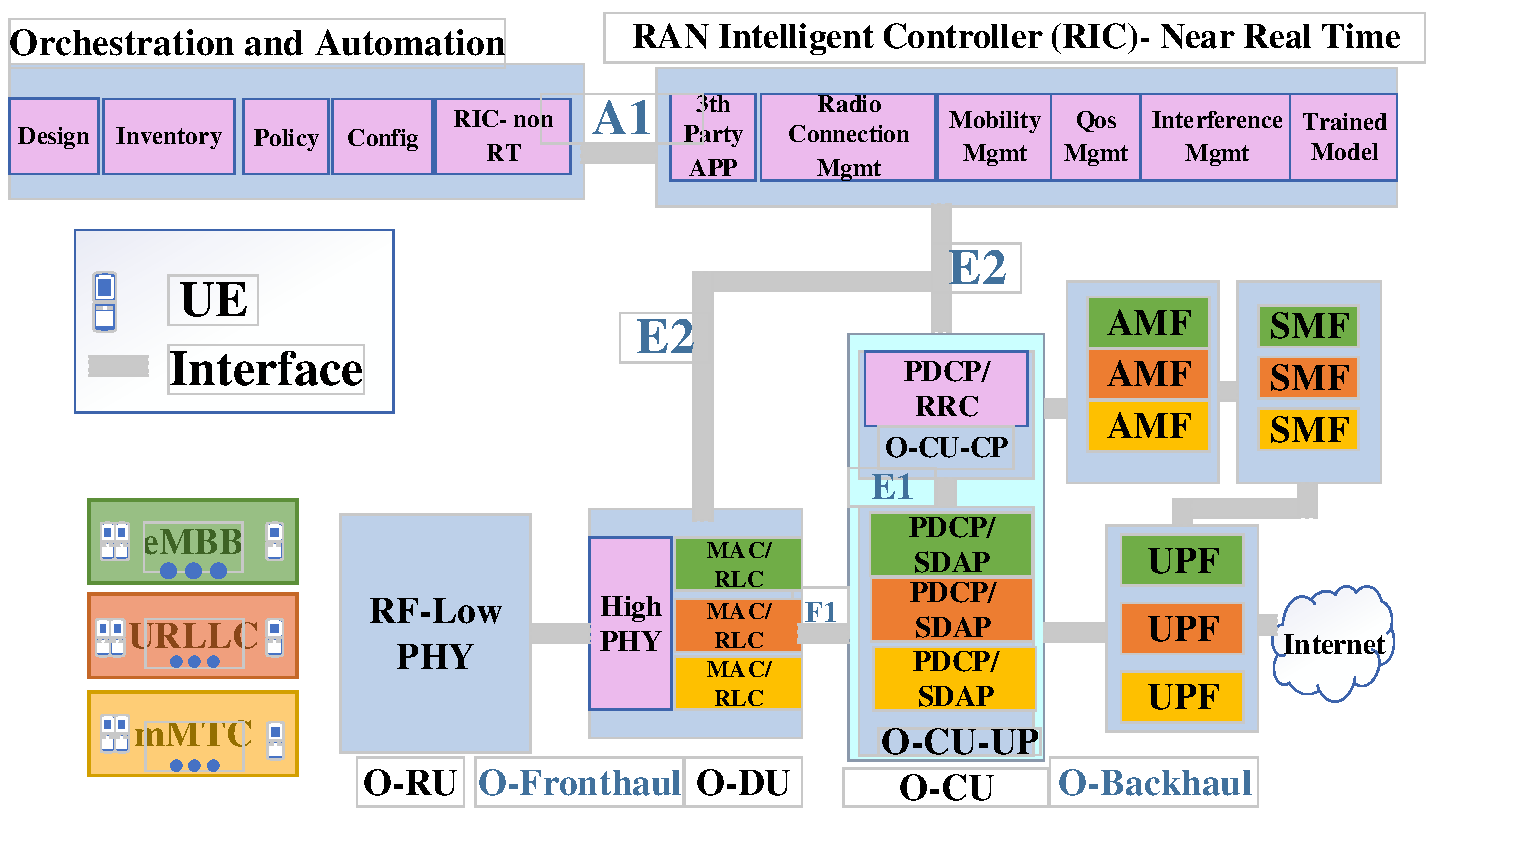
\includegraphics[scale = 0.36]{finalDraw1.pdf}
    %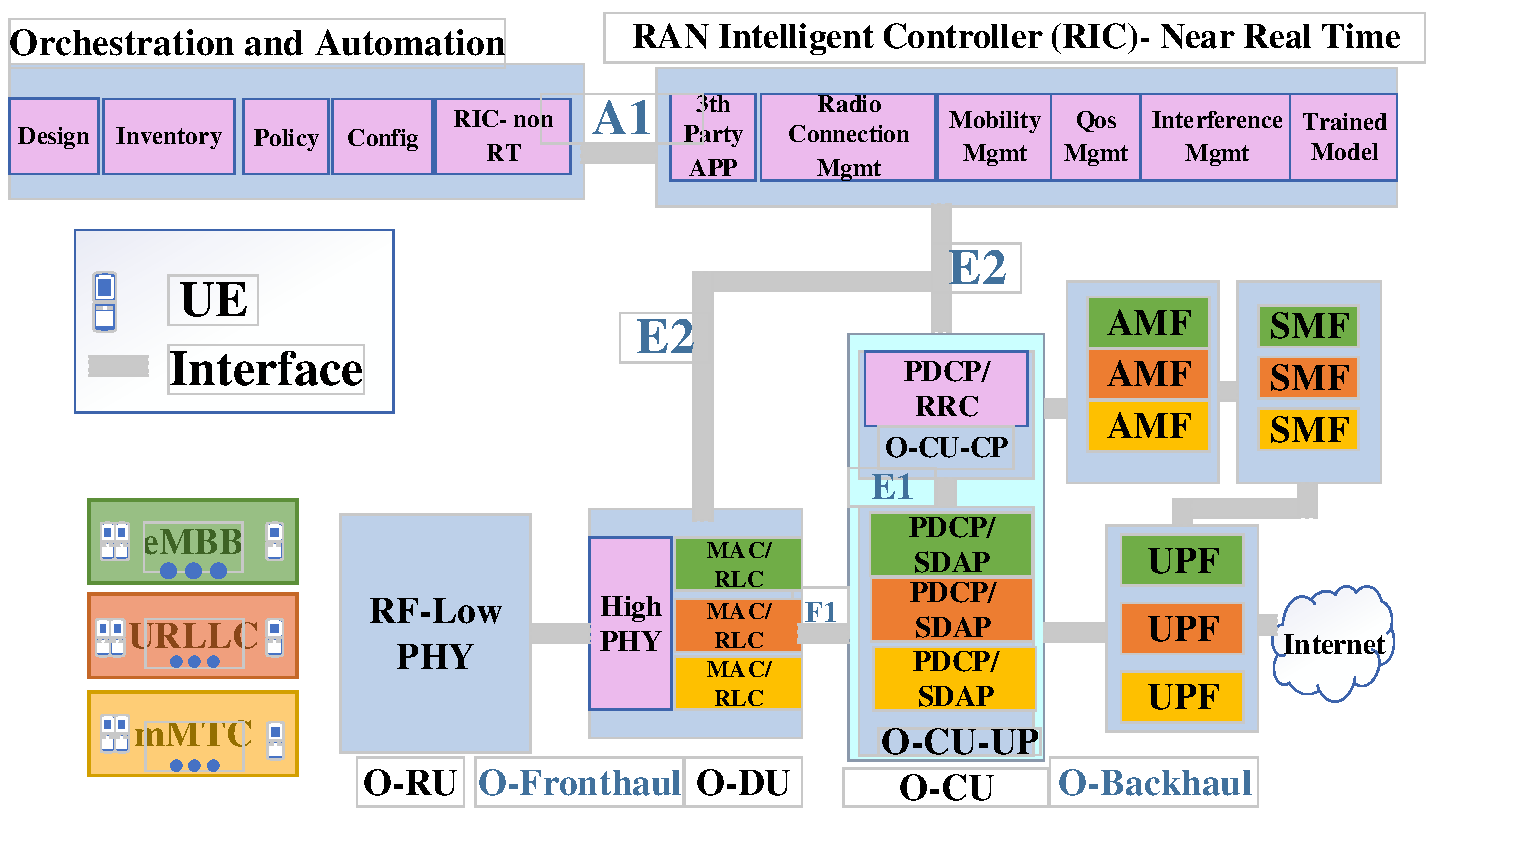
\includegraphics[width=9.cm,height=6.2cm]{finalDraw1.pdf}
    %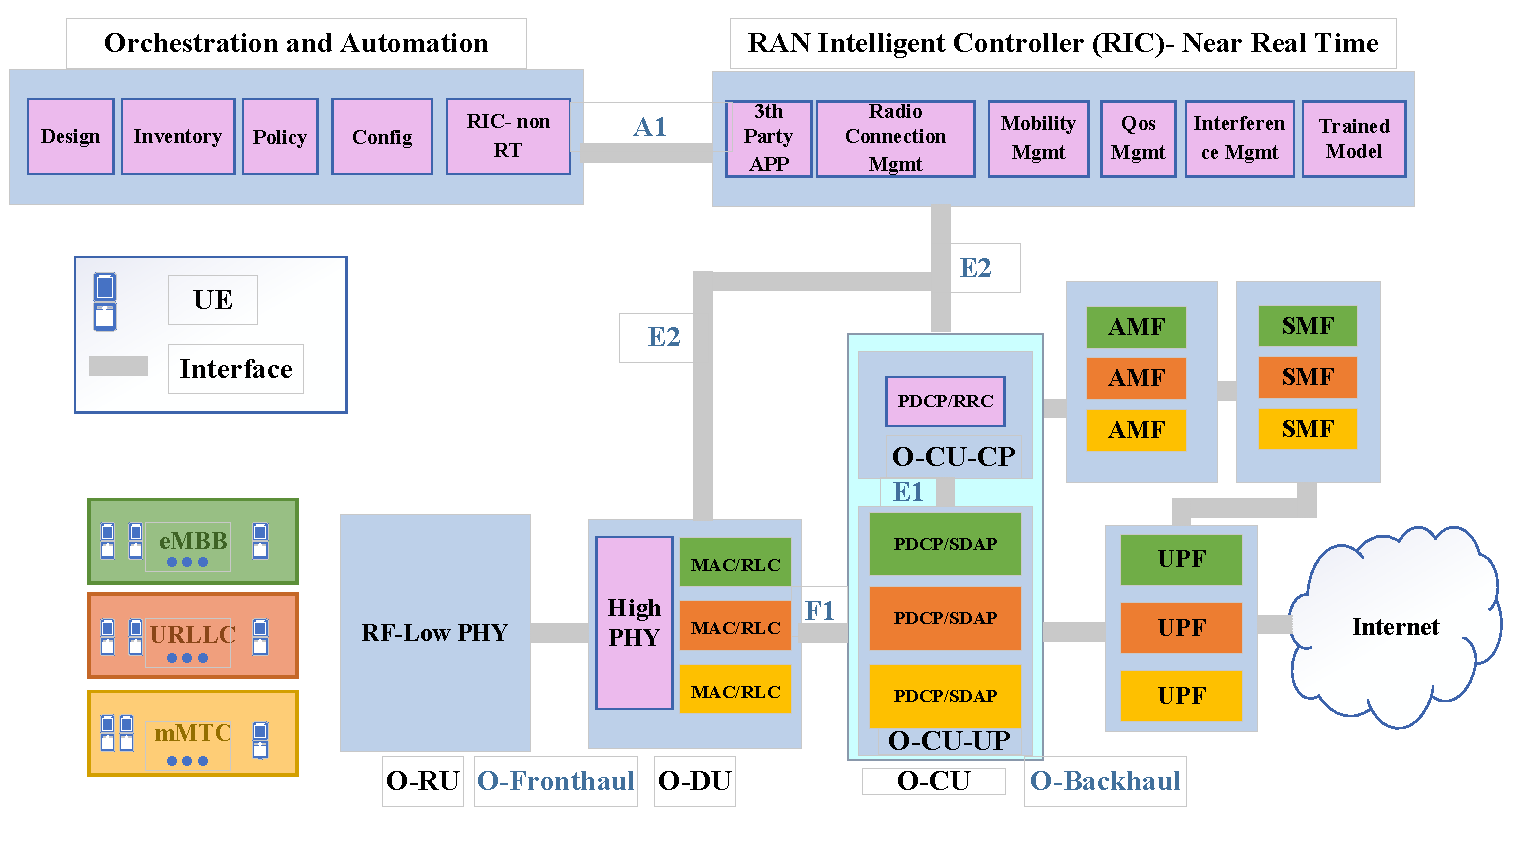
\includegraphics[width=\textwidth]{finalDraw.pdf}
  \caption{Network sliced O-RAN system}
  \label{fig:c11}
\end{figure}
O-RAN is an appropriate alternative to the next generation of radio access networks due to its flexibility, openness, low operational costs, and intelligence. 

O-RAN was developed to jointly benefit from the advantages of virtual RAN (vRAN) and cloud RAN (C-RAN).  \textcolor{MidnightBlue}{By virtualizing RANs, operators can improve flexibility, reduce CAPEX and OPEX, and add new capabilities to their networks more quickly.} The C-RAN architecture divides the RAN into two major parts: the radio remote head (RRH) and the baseband unit (BBU). Several distributed RRHs can be connected to a centralized BBU, called BBU-pool \cite{han2019research}. Unlike C-RAN, O-RAN separates RAN into three different units, namely Radio Unit (O-RU), Distributed Unit (O-DU), and Central Unit (O-CU).
 \textcolor{MidnightBlue}{Mostly non-real-time baseband processing occurs in the O-CU layer, while real-time baseband processing occurs in the O-DU layer.}

In the O-RAN architecture, the PHY is divided into low and high PHY, unlike C-RAN. As shown in Fig. \ref{fig:c11}, O-RU is a logical node that contains RF and low PHY. The former transmits or receives radio signals, while the latter includes digital beamforming. Typically, the O-DU constitutes a logical node with high PHY, MAC, and RLC. It contains a subfunction of the eNodeB and is deployed near the O-RU.
Moreover, O-DU is connected to an O-RU with an open fronthaul interface.
In addition to supporting the lower layers of the protocol stack, O-CU also provides support for the higher layers.

The O-CU contains two parts: the O-CU user plane (O-CU-UP) and the O-CU control plane (O-CU-CP). The former hosts the packet data convergence protocol (PDCP)-UP and the service data adaption protocol (SDAP), while the latter hosts PDCP-CP and radio resource control (RRC).
O-DU and O-CU are connected via an open and well-defined interface $\text{F}_1$.
Moreover, O-CU-UP is connected to user plane function (UPF) via O-backhaul link.

The O-RAN architecture contains other principal logical nodes called Orchestration and Automation, RAN Intelligent Controller (RIC)- Near Real-Time, and O-Cloud. Orchestration and Automation include functions such as RIC Non-Real-Time. RIC is responsible for machine learning methods and making the system more intelligent.

\textcolor{MidnightBlue}{A key feature of the O-
RAN architecture is that the hardware is disaggregated from
the software, leading to network function virtualization
(NFV).  Additionally, each component is implemented as a virtual network function (VNF), the system function block in NFV, that can be deployed on a virtual machine (VM) or container \cite{mijumbi2015network}. As a result, as shown in Fig \ref{fig:c11}, O-RAN components, such as UPF, O-CU, O-DU, and RIC-near real-time, are virtualized and implemented as VNFs}
\cite{gavrilovska2020cloud,niknam2020intelligent,kazemifard2021minimum,both2021system,ORANArch,ORANML,lin2021toward}. 
\vspace*{-.75em}
\section{System Model}\label{systemmodel}
We consider a downlink (DL) system, and an O-RAN architecture using RAN slicing as depicted in Fig. \ref{fig:c11}.
In this section, we present the system and signal model, derive the achievable data rates, power of O-RU, and the fronthaul capacity  of the O-RAN system. Moreover, we discuss the mean delay and the power of VNFs.
\subsection{System Model}
Assume, there are three service types: eMBB, URLLC, and mMTC, which support different applications. Accordingly, there are $S_1$ slices for the first service type (eMBB), $S_2$ slices for the second service type (URLLC), and $S_3$ slices for the third service type (mMTC).
Therefore, there are $S = S_1 + S_2 + S_3$ pre-allocated slices serving these services.
Moreover, each service request $s\in \{1,\ldots,S\}$ is served by its corresponding slice. So we have the set
$\{1,2,...,S_1\}$ of eMBB service instances, the set $\{1,2,...,S_2\}$ of URLLC service instances, and the set
$\{1,2,...,S_3\}$ of mMTC service instances.
Each service $s_j\in \{1,2,...,S_j\} $ consists of $U_{s_j}$ requests from  single-antenna UEs requiring certain level of QoS. Notice that $j \in \{1,2,3\}$ indicates the service type.
Based on the application and QoS request, UE may be admitted and allocated to the resources.

Each pre-allocated slice contains reserved VNFs for the three logical nodes:
\begin{itemize}
\item MAC/RLC functions in the O-DU 
\item PDCP/SDAP functions in the O-CU-UP
\item UPF which is a functional layer
\end{itemize}
Each slice $s \in \{1,2,...,S \}$, consists of  $M_s^{d}$ VNFs for the processing of O-DU, $M_s^{c}$ VNFs for the processing of O-CU-UP, and $M_s^{u}$ VNFs for the processing of UPF.
The VNFs of O-DU, O-CU-UP, and UPF are interconnected, which is defined as the service function chain in the O-RAN system. Also, each VNF instance runs on a VM that uses resources from the data centers.


%All $K$ PRBs can be assigned to all UEs in each service.
Assume there are $K$ PRBs in this system. Suppose each slice $s$ consists of $\bar{K}_s$ pre-allocated virtual resource blocks that are mapped to PRBs. Therefore, we have $\sum_s \bar{K}_s \leq K$.
In addition, there are $R$ multi-antenna O-RUs that are shared between the slices. Specifically, the O-RU $r \in \mathcal{R}=\{1,2,...,R \}$ has $J$ antennas for transmitting and receiving data. Moreover, all O-RUs have access to all PRBs.

%Coordinated multipoint (CoMP) system is considered here.
%\subsection{The Achievable Rate}
\subsection{Signal Model}
Let $y_{u(s,i)} $ be the received signal of UE $i$ in the $s^{th}$ service such that
\begin{equation}\label{eq2}
y_{u(s,i)} = \sum_{r = 1}^{R}\sum_{k=1}^{K_s} \boldsymbol{h}^{H \: k}_{r,u(s,i)} g_{u(s,i)}^r e^k_{r,u(s,i)}{x_Q}^k_{r,u(s,i)}+ z_{u(s,i)},
\end{equation}
%\boldsymbol{w}^k_{r,u(s,i)}p^k_{r,u(s,i)}  $\mathfrak{y}^k_{r,u(s,i)} =\boldsymbol{w}^k_{r,u(s,i)}{p^{k \: \frac{1}{2}}_{r,u(s,i)}} x_{u(s,i)}+ \boldsymbol{q}_{r}$
where ${x_Q}^k_{r,u(s,i)} ={x_P}^k_{r,u(s,i)}+ \boldsymbol{q}_{r}$. ${x_P}^k_{r,u(s,i)}= \boldsymbol{w}^k_{r,u(s,i)}\sqrt{p^{k}_{r,u(s,i)}} x_{u(s,i)} $, and  $ x_{u(s,i)}$ depicts the transmitted symbol vector, $z_{u(s,i)}\backsim \mathcal{CN}(0,BN_0)$ is the receive additive Gaussian noise and $BN_0$ is the noise power in a given bandwidth $B$.
Here, ${x_P}$ denotes the precoded message before compression, while ${x_Q}$ illustrates the precoded message after compression.% as shown in Fig. \ref{fig:pq}.
In addition, $\boldsymbol{q}_{r} \sim \backsim \mathcal{CN}(0,{\sigma_q}^2\boldsymbol{I_{R}} )$ indicates the quantization Gaussian noise which comes from the signal compression in O-DU.
Furthermore, $g_{u(s,i)}^r \in \{0,1\}$ is a binary variable that illustrates whether O-RU $r$ serves the $i^{th}$ UE that is allocated to the $s^{th}$ slice or not.
Furthermore, $p_{r,u(s,i)}^{k}$ represents the transmission power of the O-RU $r$ serve the $i^{th}$ UE in slice $s$ and PRB $k$, while
${\bold{h}_{r,u(s,i)}^{k}} \in \mathbb{C}^{J}$ corresponding channel vector.
In addition, $\bold{w}_{r,u(s,i)}^{k} \in \mathbb{C}^{J}$ depicts the associated transmit beamforming vector.
%Here, it is assumed that each UE is served by the nearest o-RU
Therefore, the SINR of the $i^{th}$ UE served at slice $s$ on PRB $k$ is given by
\begin{equation}\label{eq1}
\rho_{r,u(s,i)}^{k} =  \frac{p_{r,u(s,i)}^{k}|{\bold{h}_{r,u(s,i)}^{k \: H}} \bold{w}_{r,u(s,i)}^{k}|^2}{BN_0 + I_{r,u(s,i)}^{k}},
\end{equation}

A UE in an O-RU $r$ using PRB $k$ receives interference from other O-RUs in the set $\mathcal{R}\backslash r$ that are using the same PRB $k$. Two types of interference occur between UEs in each slice: i) inter-slice interference between signals transmitted over different slices, and ii) intra-slice interference between signals transmitted over the same slice.%that is shown in Fig. \ref{fig:intf}.
 
Network slicing techniques significantly reduce inter-service (inter-slice) interference.
One way to leverage a two-time scale PRB scheduling is to isolate PRBs in slices (in the first time scale) and schedule the PRBs to the UEs of the slices (in the second time scale). Another method consists of allocating part of the PRBs of eMBB services to URLLC and mMTC \cite{alsenwi2021intelligent, setayesh2020joint, mei2021intelligent}. In this paper, we assume that the PRB scheduling is performed. Also, in Section \ref{prb}, we briefly study the PRB scheduling between slices.
Since there are limited resources, inter-service interference cannot be eliminated entirely. Nevertheless, isolating the slices reduces inter-service interference considerably and allows us to ignore it mathematically.
%\begin{figure}
%  \centering
%  \captionsetup{justification=centering}
%    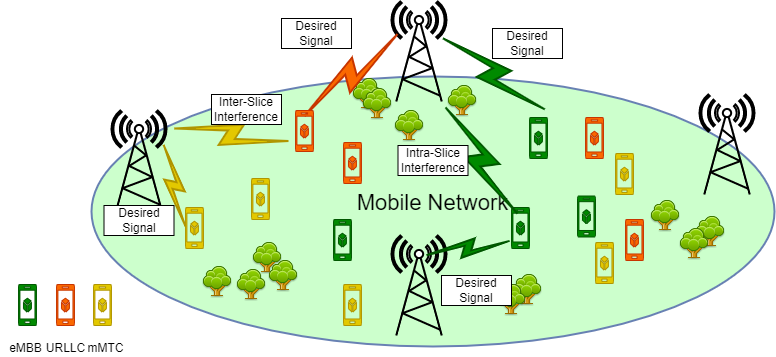
\includegraphics[scale = 0.35]{Interference.png}
%    %\includegraphics[max height=30cm,max width=9.5cm]{Drawing15.eps}
%    %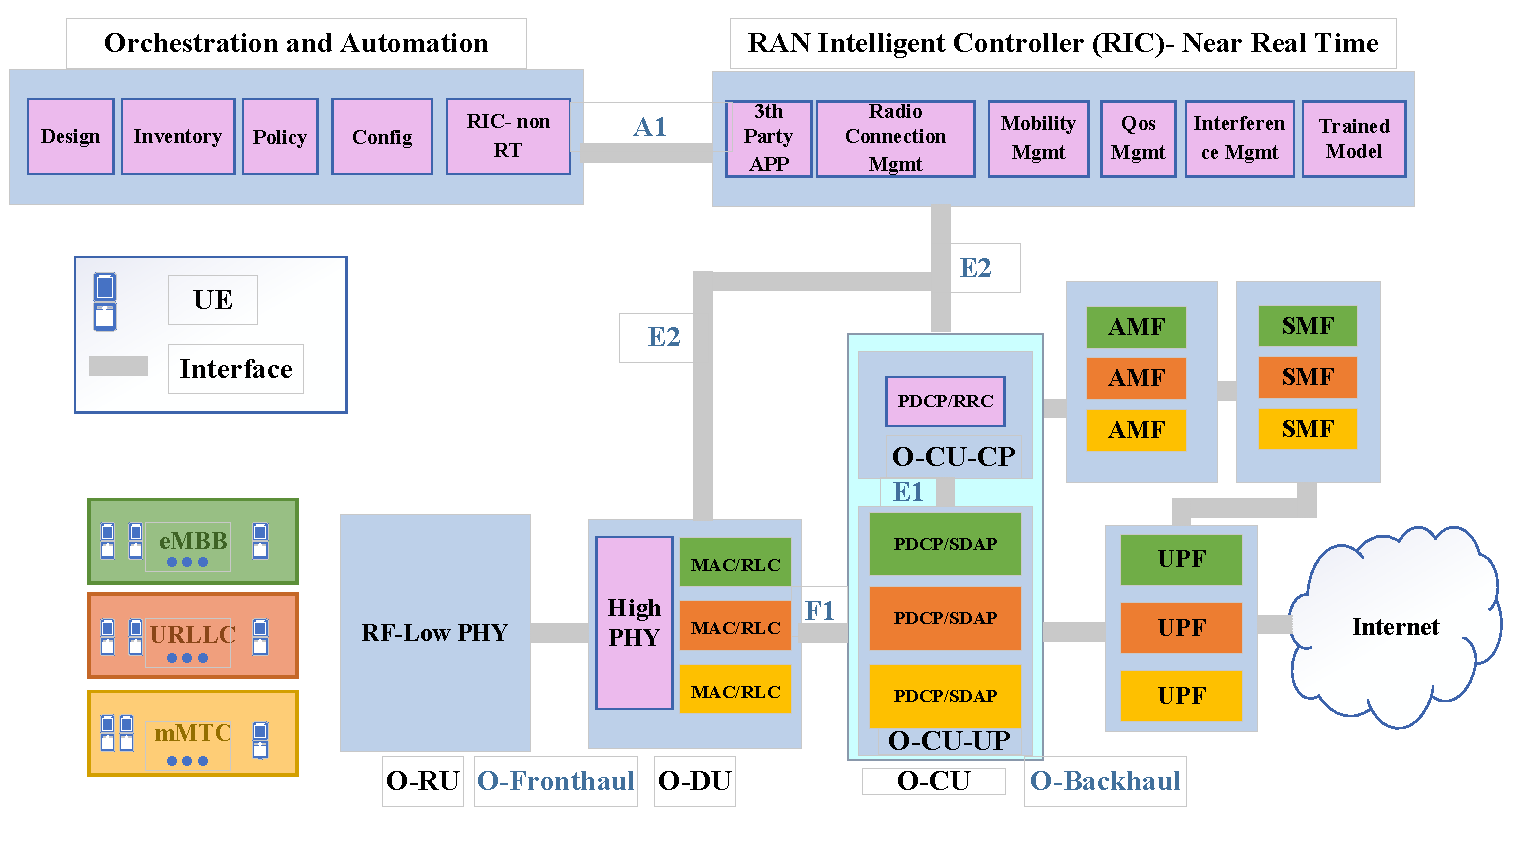
\includegraphics[width=\textwidth]{finalDraw.pdf}
%  \caption{Type of Interference Signal}
%  \label{fig:intf}
%\end{figure}

Back to \eqref{eq1}, $I_{r,u(s,i)}^{k}$ is the sum of the power of interfering signals and quantization noise, and can be represented as 
%{\color{red} use paranthesis in the following equation to clear +}
%\begin{subequations}\label{eqI}
%\begin{alignat}{4}
%\begin{align}\label{eqI}
%&I_{r,u(s,i)}^{k} =\nonumber\\
% &\underbrace{\sum_{\substack{l=1 \\ l\neq i}}^{{U}_{s}} e^{k}_{u(s,i)}e^{k}_{u(s,l)}  p_{u(s,l)}^{k}\sum_{\substack{r'=1 \\ r'\neq r}}^{R}|{\bold{h}_{r',u(s,i)}^{k \: H}} \bold{w}_{r',u(s,l)}^{k} g_{u(s,l)}^{r'}|^2}_{\text{(intra-slice interference)}}+\nonumber\\
%&\underbrace{\sum_{\substack{n = 1 \\ n\neq s}}^{S}\sum_{l=1}^{{U}_s} e^{k}_{u(s,i)}e^{k}_{u(n,l)}  p_{u(n,l)}^{k}\sum_{\substack{r'=1 \\ r'\neq r}}^{R}|{\bold{h}_{r',u(s,i)}^{k \: H}} \bold{w}_{r',u(n,l)}^{k} g_{u(n,l)}^{r'}|^2}_{\text{(inter-slice interference)}}\nonumber\\
%&+\underbrace{  \sum_{j=1}^{{R}} {\sigma_q}^2 |\boldsymbol{h}_{r,{u(s,i)}}^k|^2 }_{\text{(quantization noise)}},
%\end{align}
%\end{alignat}
%\end{subequations}
%{\color{red} $\gamma_1$ is constant used instead of variable. }
\begin{align}\label{eqI}
&I_{r,u(s,i)}^{k} =\underbrace{  \sum_{j=1}^{{R}} {\sigma_q}^2 |\boldsymbol{h}_{r,{u(s,i)}}^k|^2 }_{\text{(quantization noise)}} + \nonumber\\
 &\underbrace{\sum_{\substack{l=1 \\ l\neq i}}^{{U}_{s}} e^{k}_{u(s,i)}e^{k}_{u(s,l)}  p_{u(s,l)}^{k}\sum_{\substack{r'=1 \\ r'\neq r}}^{R}|{\bold{h}_{r',u(s,i)}^{k \: H}} \bold{w}_{r',u(s,l)}^{k} g_{u(s,l)}^{r'}|^2}_{\text{(intra-slice interference)}},
\end{align}
%where $\gamma_{1} = e^{k}_{u(s,i)}e^{k}_{u(s,l)}$ and $\gamma_{2} = e^{k}_{u(s,i)}e^{k}_{u(n,l)}$.
where $e^{k}_{u(s,i)}$ is a binary variable that indicates whether the $k^{th}$ PRB is allocated to the UE $i$ in slice $s$, assigned to $r^{th}$ O-RU, or not. %($\gamma_1$ and $\gamma_2$ are two variales. You  define on variable here.)
Furthermore, there is no inter-slice interference, only intra-slice interference, since slices are assumed to be isolated. 

%To obtain SNR as formulated in \eqref{eq1}, 
%\begin{figure}
%  \centering
%  \captionsetup{justification=centering}
%    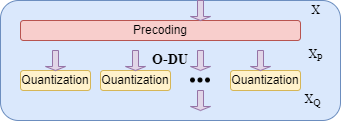
\includegraphics[scale = 0.45]{Qdiag.png}
%    %\includegraphics[max height=30cm,max width=9.5cm]{Drawing15.eps}
%    %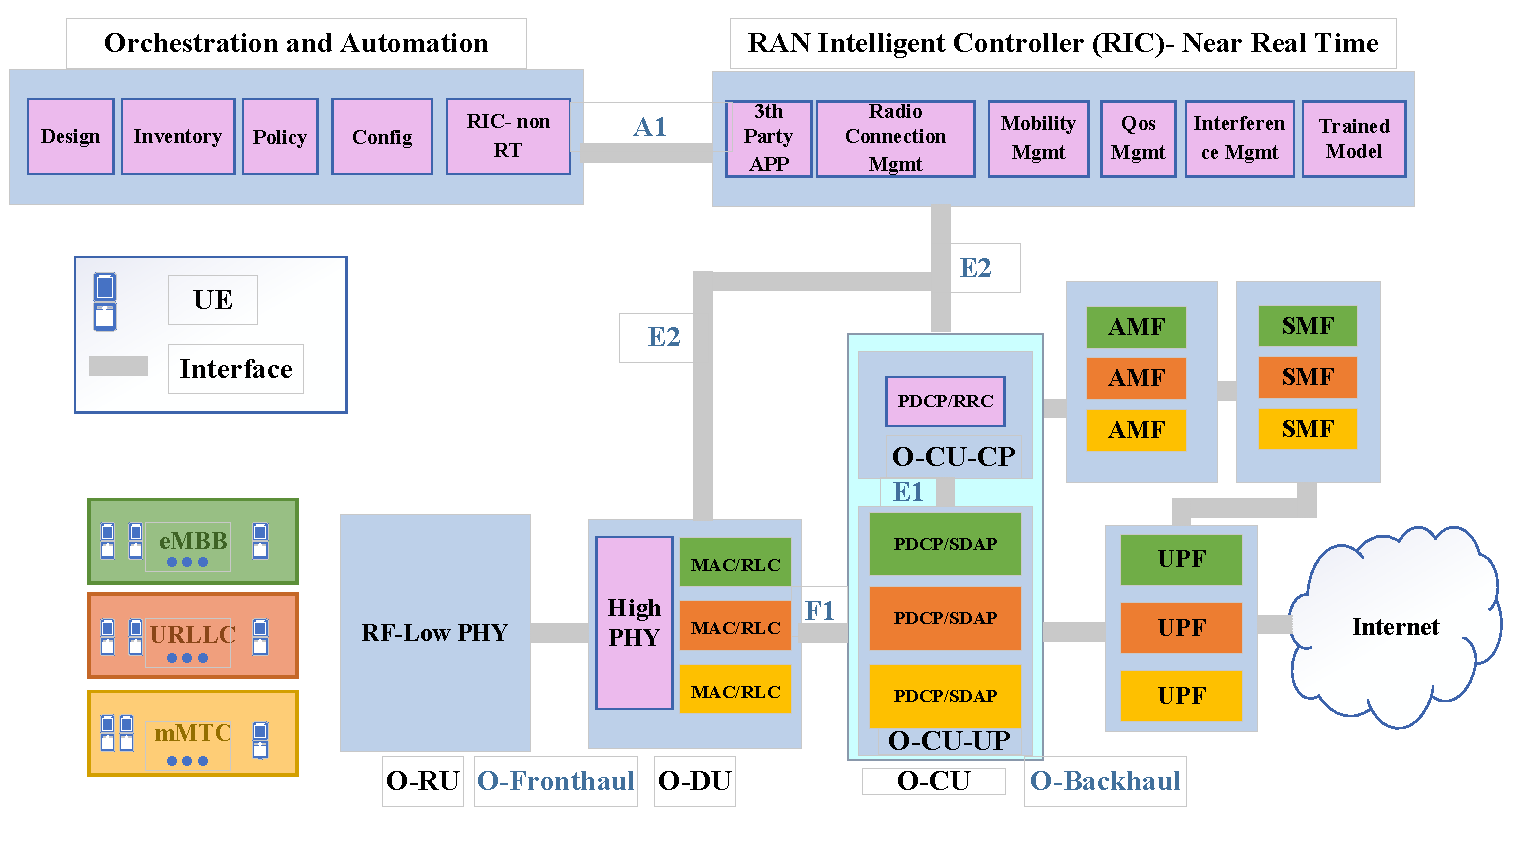
\includegraphics[width=\textwidth]{finalDraw.pdf}
%  \caption{Precoding and Quantization of Signal}
%  \label{fig:pq}
%\end{figure}

 Herein, we consider a zero forcing beamforming vector, which minimizes the experienced intra-slice interference, and is given by \cite{huang2013user}
\begin{equation}
\bold{w}_{r,u(s,i)}^{k} = \hat{\bold{h}}_{r,u(s,i)}^{k}(\hat{\bold{h}}_{r,u(s,i)}^{k \: H} \hat{\bold{h}}_{r,u(s,i)}^{k})^{-1}.
\end{equation}
\noindent where $\bold{h}_{r,u(s,i)}^{k}$ is the channel estimate, which is assumed imperfect. Mathematically,
$\hat{\boldsymbol{h}}_{r,u(s,i)} = \boldsymbol{h}_{r,u(s,i)} + \Delta \boldsymbol{h}_{r,u(s,i)}$, where
$\Delta \boldsymbol{h}_{r,u(s,i)}\sim \mathcal{N}(0,\boldsymbol{\phi}_{r,u(s,i)}^2)$ indicates the estimating error vector with a Gaussian distribution and $\boldsymbol{\phi}_{r,u(s,i)} = \text{diag}(\phi_{r,u(s,i)},\ldots,\phi_{r,u(s,i)}).$
\vspace*{-.8em}
\subsection{Achievable Data Rate}
The achievable data rate for the $i^{th}$ UE request in the $s_{1}^{th}$ application of service type 1 (eMBB) can be written as 
\begin{equation}\label{eq3}
\mathcal{R}_{u(s_1,i)} = \sum_{r=1}^{R}\mathcal{R}_{r,u(s_1,i)} g^r_{u(s_1,i)},
\end{equation}
where
\begin{equation}
\mathcal{R}_{r, u(s_1,i)} = \sum_{k=1}^{K} \mathcal{{R}}_{r,u(s_1,i)}^{k} e^k_{r,u(s_1,i)},
\end{equation}
is the achievable data rate of RU $r$ to UE $i$ in slice $s_1$, which depends on the achievable data rate per PRB, i.e.,
\begin{equation}
\mathcal{{R}}_{r,u(s_1,i)}^{k} =  B \log_2({1+ \rho_{r,u(s_1,i)}^{k}}),
\end{equation}
%\begin{subequations}\label{eq3}
%\begin{alignat}{4}
%\mathcal{{R}}_{r,u(s_1,i)}^{k} &=  B \log_2({1+ \rho_{r,u(s_1,i)}^{k}}) ,\\
%\mathcal{R}_{r, u(s_1,i)} &= \sum_{k=1}^{K} B \log_2({1+ \rho_{r,u(s_1,i)}^{k}} e^k_{r,u(s_1,i)}),\\
%\mathcal{R}_{u(s_1,i)} &= \sum_{r=1}^{R}\mathcal{R}_{r,u(s_1,i)} g^r_{u(s_1,i)},
%\end{alignat}
%\end{subequations}
Since the blocklength in URLLC and mMTC is finite, the achievable data rate for the $i^{th}$ UE request in the application of service type 2 (URLLC) and 3 (mMTC) is not achieved from the Shannon capacity formula. Instead, in a short packet transmission, the achievable data rate is approximated as \cite{setayesh2020joint}
\begin{equation}\label{eq11}
\mathcal{R}_{u(s_j,i)} = \sum_{r=1}^{R}\mathcal{R}_{u(s_j,i)}^{r} g^r_{u(s_j,i)},
\end{equation}
where
\begin{equation}
\mathcal{R}_{r,u(s_j,i)} = \mathcal{{R}}_{r,u(s_j,i)}^{k}{e}_{u(s_j,i)}^{k},
\end{equation}
is the achievable data rate of RU $r$ to UE $i$ in slice $s_1$, which depends on the achievable data rate per PRB, i.e.,
\begin{equation}
\mathcal{{R}}_{r,u(s_j,i)}^{k} = B \log_2({1+ \rho_{r,u(s_j,i)}^{k}} - \zeta_{u(s_j,i)}^{k}){e}_{u(s_j,i)}^{k},
\end{equation}
%\begin{subequations}\label{eq11}
%\begin{alignat}{4}
%\mathcal{{R}}_{r,u(s_j,i)}^{k} &= B \log_2({1+ \rho_{r,u(s_j,i)}^{k}} - \zeta_{u(s_j,i)}^{k}){e}_{u(s_j,i)}^{k},\\
%\mathcal{R}_{u(s_j,i)}^{r} &= \sum_{k=1}^{K} B (\log_2({1+ \rho_{u(s_2,i)}^{k}})- \zeta_{u(s_j,i)}^{k}){e}_{u(s_j,i)}^{k},\\
%\mathcal{R}_{u(s_j,i)} &= \sum_{r=1}^{R}\mathcal{R}_{u(s_j,i)}^{r} g^r_{u(s_j,i)},
%\end{alignat}
%\end{subequations}
where %$j \in \{2,3\}$. Also we have $ \zeta_{u(s_j,i)}^{k} = \log_2({e})Q^{-1}(\epsilon) \sqrt{\frac{\mathfrak{C}_{u(s_j,i)}^{k}}{N_{u(s_j,i)}^{k}}},$.
%{\color{red} check paranthesis. }
\begin{equation}\label{shortPacket}
 \zeta_{u(s_j,i)}^{k} = \log_2({e})Q^{-1}(\epsilon) \sqrt{\frac{\mathfrak{C}_{u(s_j,i)}^{k}}{N_{u(s_j,i)}^{k}}}.
\end{equation}
%{\color{red} what is transmission probability? }
Here, $\epsilon$ is the transmission error probability, $Q^{-1}$ is the inverse of the Q function,
$\mathfrak{C}_{u(s_j,i)}^{k} = 1 - \frac{1}{(1+\rho_{u(s_j,i)}^{k})^2}$ depicts the channel dispersion of UE  $i$ at slice $s_j$ and PRB $k$, while
$N_{u(s_j,i)}^{k}$ represents the corresponding transmit blocklength.
$\mathcal{R}_{r,u(s_j,i)}$ is the achievable data rate that is transmitted by O-RU $r$ to UE $i$ requesting service $s_j$.

If we replace $p_{u(s,l)}^{k}$ and $p_{u(n,l)}^{k}$ in \eqref{eqI} by $P_{s}^{\text{max}}$, an upper bound $\bar{I}_{r,u(s,i)}^{k}$ is obtained for $I_{r,u(s,i)}^{k}$. Therefore, $\bar{\mathcal{R}}_{u_{(s,i)}} \forall s , i$ is derived by using $\bar{I}_{r,u(s,i)}^{k}$ instead of $I_{r,u(s,i)}^{k}$ in  \eqref{eq11} and \eqref{eq3}.
\subsection{Power of the O-RU and the Fronthaul Capacity}
Let $P_r$ denote the power of the transmitted signal from the $r^{th}$ O-RU to all the UEs served by it. From \eqref{eq2}, the power of each O-RU $r$ is obtained as follows,
%{\color{red} is this the sum rate of all users?}
\begin{equation}\label{pr}
P_r = \sum_{s=1}^{S}\sum_{k=1}^{K_s}\sum_{i=1}^{U_s}|\bold{w}_{r,u(s,i)}^{k}|^2\alpha^k_{r,u(s,i)} + \sigma_{q}^2,
\end{equation}
where $\alpha^k_{r,u(s,i)}= p_{r,u(s,i)}^{k} g_{u(s,i)}^r e^k_{r,u(s,i)}$.
Since we have a fiber link between O-RU and O-DU, the rate of users on the fronthual link between O-DU and the $r^{th}$ O-RU  is formulated as
%\cite{simeone2016cloud, 1111}
\begin{align}\label{cr}
C_{r} &= \log{\left(1+ \frac{\sum_{s=1}^{S}\sum_{k=1}^{K_s}\sum_{i=1}^{U_s}|\bold{w}_{r,u(s,i)}^{k}|^2 \mathcal{\alpha}^k_{r,u(s,i)} }{ \sigma_{q}^2}\right)},\nonumber\\
C_{r} &= \log_2{\left(\frac{P_r}{ \sigma_{q}^2}\right)}.
\end{align}
\subsection{Mean Delay}
In this part, the end-to-end mean delay for each service is obtained.
The total delay ($T^{\text{\text{tot}}}$), is the sum of the processing delay ($T^{\text{proc}}$), the transmission delay ($T^{tr}$), and the total propagation delay ($T^{\text{pro}}$).
\begin{subequations}
\begin{alignat}{4}
T^{\text{\text{tot}}} &=  T^{\text{proc}} + T^{tr} + T^{\text{pro}},\\
T^{\text{\text{proc}}} &=  T^{\text{RU}} + T^{\text{DU}} + T^{\text{CU}} + T^{\text{UPF}},\\
T^{\text{tr}} &= T^{\text{fr},t} + T^{\text{mid},t} + T^{\text{b},t},  \\
T^{\text{pro}} &= T^{\text{fr},p} + T^{\text{mid},p} + T^{b,p}.
\end{alignat}
\end{subequations}
%{\color{red} I made a mistake and replaced pro with proc. Please correct them. Also, explain in more details the processing delay in this paragraph.}
%T_{\text{\text{tot}}} = T_{RU} + T_{front} + T_{DU} + T_{\text{mid}} + T_{CU} + T_{back} + T_{core} + T_{trans2net}
Mathematically, the total propagation delay ($T^{\text{pro}}$) is the sum of the propagation delay in the fronthaul link $T^{fr,p}$, the midhaul link $T^{\text{mid},p}$, and the backhaul link $T^{b,p}$. In each link, the propagation delay is the time a signal to reach its destination. It is obtained based on the length of the fiber link and the capacity of the link (as $\text{T} = \text{L}/\text{c}$, where L is the length of the link and c is the propagation speed of the medium).
Meanwhile, the total transmission delay ($T^{tr}$) is the sum of the transmission delay in the fronthaul $T^{fr,t}$, the midhaul $T^{\text{mid},t}$, and the backhaul $T^{b,t}$.
In each link, the transmission delay is the amount of time required to push all the packets into the transmission medium, and can formulated as
$T = \frac{\mathcal{\alpha}}{R}$, where $R$ is the data-rate of the packet and $\mathcal{\alpha}$ is the mean packet size.
Notice that taking the propagation and transmission delays into account in the formulation is straightforward, but we have avoided it for the sake of succinctness and simplicity.
%It is worth highlighting that propagation delay must be specially considered when each O-RU can connect to several number of O-DUs and depending on the route, capacity, and priority. 
%However, this would provide a new problem formulation, which could be added to our system model to extend our paper in the future. In the current paper, we assume that the connection between O-RUs and O-DUs is fixed and transparent, and we do not consider the problem of edge processing. 
Therefore, the propagation delay is fixed and does not affect the optimization problem. 

Next, we present a brief calculation of propagation delay.
Assume a distance between the O-RU and O-DU around 10 km, the distance between O-DU and O-CU around 80 km, not greater than the distance from O-CU to the network around 200 km \cite{oranD1}. Then, assuming the fronthaul, midhaul and backhaul are connected with fiber optics and $c$ is the speed of like, the propagation delay is about $T^{\text{pro}} = (10 + 80 + 200)\times 10^3 /(3\times 10^8) < 1$ ms.

The following is a brief calculation of transmission delay to show that it does not affect also the optimization since its contribution to the total delay is negligible.
In URLLC and mMTC, the mean packet size can be between 20 to 32 bytes; Also, the minimum data rate is assume to be $1 bps/Hz \times BW (180 KHz)$. So the transmission delay from O-RU to O-DU is about $T^{fr,t} = \frac{20\times 8}{1 \times 180 \times 10^3} < 0.1 ms$. As a result, the $T^{fr,t} \approx T^{mid,t} \approx T^{b,t}$. For eMBB, the packet size can be 100 times larger and the delay is not exceed the 0.6ms.


Therefore, in the following, we assume that the total delay is approximate to the processing delay ($T^{\text{\text{tot}}} \approx T^{\text{proc}}$).
%Here we assume the propagation delay and the transmission delay are negligible compared to the processing delay.
%\begin{equation}
%T^{\text{\text{tot}}} \approx T^{\text{proc}}
%\end{equation}
\subsubsection{Processing Delay}
Assume the packet arrival of UEs follows a Poisson process with arrival rate $\lambda_{u(s,i)}$ for the $i^{th}$ UE of the $s^{th}$ service (or slice).
Therefore, the mean arrival data rate of the $s^{th}$ slice in the UPF layer is $\alpha_{s}^U = \sum_{u=1}^{U_s}\lambda_{u(s,i)}$.
Assume the mean arrival data rate of the UPF layer for slice $s$ ($\alpha_{s}^U$) is approximately equal to the mean arrival data rate of the O-CU-UP layer ($\alpha_{s}^C$) and the O-DU ($\alpha_{s}^D$), i.e., $\alpha_{s} =\alpha_{s}^U \approx \alpha_{s}^C \approx \alpha_{s}^D$. This is because the amount of data transferred along the route (regardless of frame changes) is constant.
In fact, according to Burke’s theorem, the mean arrival data rate of the second and third layers, which are processed in the first layer, is still Poisson with rate $\alpha_{s}$.
It is assumed that there are load balancers in each layer for each service to divide equally the incoming traffic to VNFs. %\cite{frdl,luong2018novel,luong2018novel1}.
Suppose the baseband processing of each VNF is modeled by an M/M/1 processing queue.
%Since the system's arrival packets are from many independent sources. Moreover, the impact of a single packet on the system's performance is minimal. Also, the queue discipline will be first-in, first-out (FIFO), and the arrival packet is assumed to follow a Poisson process. Therefore, we suppose that service times are exponentially distributed [36]. In addition, since the services are isolated, the UEs in each service have the same priority, and the processing delays of each service are independent of the other services; Therefore, one service could have a higher priority, affecting the whole optimization, and the M/M/1 queue theory is still validated.
Each packet is processed by one of the VNFs of the corresponding slice. Therefor, the mean delay for the $s^{th}$ slice in the O-DU, the O-CU, and the UPF is modeled as M/M/1 queue, and can be respectively \cite{SystemCostMinimization,luong2018joint,luong2018novel},
\begin{align}
T_{s}^{\text{DU}} &= \frac{1}{\mu_s^d - \alpha_{s}/{M_s^{d}}},\\
T_{s}^{\text{CU}} &= \frac{1}{\mu_s^c - \alpha_{s}/{M_s^{c}}},\\
T_{s}^{\text{UPF}} &= \frac{1}{\mu_s^u - \alpha_{s}/{M_s^{u}}},
\end{align}
where $M_s^{d}$, $M_s^{c}$ and
$M_s^{u}$ represent the number of VNFs in O-DU, O-CU-UP and UPF, respectively.
Moreover, $1/\mu_s^d$, $1/\mu_s^c$, and $1/\mu_s^u$ are the mean service time of the O-DU, O-CU, and the UPF layers, respectively. The arrival rate of each VNF in each layer for each slice
$s$ is $\alpha_{s}/{M_s^{i}}$ $ i \in \{d,c, u\}$.

On the other hand, arrival data rate of wireless link for each UE $i$ of service $s$ is $\lambda_{u(s,i)}$, thus $\sum_{i = 1}^{U_s} \lambda_{u(s,i)} = \alpha_s$.
Moreover, the service time of transmission queue for UE $i$ requesting service $s$ has
an exponential distribution with mean $1/R_{u(s,i)}$ and can be modeled as a M/M/1 queue \cite{SystemCostMinimization,luong2018joint,luong2018novel}.
Therefore, the mean delay of the transmission layer for UE $i$ in slice $s$ is
\begin{equation}
 T_{u(s,i)}^{\text{RU}} = \frac{1}{R_{u(s,i)} - \lambda_{u(s,i)}}.
\end{equation}
we assume $T^{\text{\text{tot}}}_{u(s,i)} \approx T^{\text{proc}}_{u(s,i)} $. %{\color{red} what results in this approximation?}
%Furthermore, the mean arrival data rate of the each link ($\textstyle \alpha_{s}^i$ , $i \in \{RU,DU,CU,UPF\}$) is approximately equal to others ($\textstyle \alpha_{s} \approx \alpha_{s}^i$ , $i \in \{RU,DU,CU,UPF\}$).
\subsection{VNF Power}
%{\color{red} Assume the power consumption of the baseband processing, the VNFs cost of a slice $s$ is depicted as $\phi_{s}$. Sentence has no meaning.}
Assume the power consumption of each VNF in each logical node (O-DU, O-CU, and UPF) in the slice s, is represented by $\phi_{s}^d$, $\phi_{s}^c$, and $\phi_{s}^u$, respectively.
Then, the system's total cost of energy of all the slices can be represented as $\textstyle \phi_{\text{\text{tot}}} = \sum_{s=1}^{S}\phi_{s}$,
%\begin{equation*}
%\textstyle \phi_{\text{\text{tot}}} = \sum_{s=1}^{S}\phi_{s},
%\end{equation*} and $\phi_{s}$ is obtained from $\phi_{s} = M_s^u \phi_s^u + M_s^c \phi_s^c+ M_s^d \phi_s^d.$
%\begin{equation}
%\phi_{s} = M_s^u \phi_s^u + M_s^c \phi_s^c+ M_s^d \phi_s^d.
%\end{equation}

A significant issue facing the industry is reducing energy consumption. Data centers are one of the most energy-consuming. As a result, restrictions are placed on data centers' energy, including VMs. So, one of our goals is to limit the energy consumption of total VNFs that can be run as VM on data centers. So, by applying a custom policy on total power consumption, we can control data centers' power consumption ($\phi^{\text{\text{tot}}}  \leq \phi^{\text{max}}$).
\section{Problem Statement} \label{prS}
Suppose the slice $s$ (which is assigned to service s) has a priority factor $\delta_s$ (based on the priority of its hosting service) where $\sum_{s=1}^S \delta_s =1$.
The priority factor of each slice is obtained according to the service level agreement to promote a fairness in the system.
%{\color{red} explain why you introduce priority factor.}
This paper aims to maximize the sum-rate of all UEs subject to QoS constraints as follows. %{\color{red} where did you define the objective? what is R bar?}
\begin{subequations}\label{problem}
\begin{alignat}{4}
\max\limits_{\boldsymbol{P}, \boldsymbol{E}, \boldsymbol{M}, \boldsymbol{G} }   \quad &  \sum_{s=1}^{S}\sum_{i=1}^{U_s}\delta_s \bar{\mathcal{R}}_{u_{(s,i)}} \ \\
\text{subject to} \quad  &  P_r \leq P^{\text{max}}_{r} \quad \forall r,
 \label{c11} \\
&p_{r,u(s,i)}^{k}  \geq 0  \quad \forall i, r, s, k,\label{c12} \\
&p_{r,u(s,i)}^{k}  \leq P_{s}^{\text{max}}  \quad \forall i, r, s, k,\label{c12-1} \\
&\bar{\mathcal{R}}_{u_{(s,i)}} \geq \mathcal{R}_{{s}}^{\min} \quad \forall s, \label{c13} \\
%&\mathcal{R}_{u_{(s_2,i)}}^u \geq  \mathcal{R}_{min}^{s_2,u} \quad \forall s_2, \label{c14} \\
& C_r \leq C^{\text{max}}_r \quad \forall r, \label{c15}\\
&T^{\text{\text{tot}}}_{u(s,i)}  \leq T^{\text{max}}_{s} \quad \forall i, s,\label{c16} \\
& \mu_s \geq \alpha_s/M_s \quad \forall s,\label{c16-1} \\
& \bar{\mathcal{R}}_{u_{(s,i)}} \geq {\lambda}_{u_{(s,i)}} \quad \forall i, s,\label{c16-2} \\
& 0 \leq M_s \leq M^{\text{max}}_s  \quad \forall s,\label{c16-3}\\
& \phi^{\text{\text{tot}}}  \leq \phi^{\text{max}}, \label{c19} \\
%& P_r\{E_1, E_2, E_3, E_4\} \leq \epsilon_s \quad \forall s_2, \label{c166}\\
& \sum_{r}g^r_{u(s,i)} = 1  \quad \forall s, i, \label{c17}  \\
& \sum_{k =1}^{K_s} g^r_{u(s,i)} e^{k}_{r,u(s,i)} \geq 1  \quad \forall s, i , r, \label{c18-1} \\
& \sum_{s =1}^{S}\sum_{i=1}^{U_s}g^r_{u(s,i)} e^{k}_{r,u(s,i)} \leq 1  \quad \forall s, i , r, \label{c18} \\
& g^r_{u(s,i)} \in \{0,1\} \quad \forall s, i, \label{c20}  \\
& e^k_{r,u(s,i)} \in \{0,1\} \quad \forall s, i. \label{c21}
\end{alignat}
\label{constraints}
\end{subequations}
\noindent \noindent where $\bar{\mathcal{R}}_{u_{(s,i)}}$ is derived by using $\bar{I}_{r,u(s,i)}^{k}$ instead of $I_{r,u(s,i)}^{k}$ in  \eqref{eq11} and \eqref{eq3}.
In addition, $\boldsymbol{P} =[p_{r,u(s,i)}^{k}], \:\: \forall s , i, r, k $, is the four-dimensional (4D) matrix of power for UEs, $\boldsymbol{E} =[e_{r,u(s,i)}^k], \:\: \forall s , i, r, k$ indicates the binary 4D matrix for the PRB association. Moreover, $\boldsymbol{G} =[g_{u(s,i)}^r], \:\: \forall s , i, r$ is a binary three dimensional (3D) matrix for the O-RU association. Furthermore, $M = [M_s^d, M_s^c, M_s^u], \:\: \forall s$ is a matrix containing the number of VNFs in each layer of slice. Notice that 
\eqref{c11}, \eqref{c12} and \eqref{c12-1} limit the power of each O-RU and UE.
Also, \eqref{c13} constrains the rate of each UE requesting each type of service, i.e., eMBB, mMTC, and URLLC, to be greater than a threshold. Meanwhile,
\eqref{c15} and \eqref{c16} represent the limited fronthaul capacity and the limited end-to-end delay of the received signal, respectively.
\eqref{c16-1} and \eqref{c16-2} are related to the stability of the M/M/1 queue,
\eqref{c16-3} restrictes the number of VNFs in each slice due to the limited resources, while
%\eqref{c16} is a reliability condition that the delay in each layer should be less than the threshold.
\eqref{c17} and \eqref{c18-1} guarantee that the O-RU and PRB are associated with the UE, respectively.
Also, \eqref{c18} ensures that each PRB can not be assigned to more than one UE associated with the same O-RU, \eqref{c19} indicates that the fixed cost of energy of VNFs in each slice does not exceed the threshold, while \eqref{c20} and \eqref{c21} constrain $\boldsymbol{E}$ and $\boldsymbol{G}$ to be binary matrices.
\subsection{PRB Scheduling}\label{prb}
In this section, we provide a brief study on the problem of PRB scheduling which can be completed in two steps to eliminate the inter-slice interference and guarantee the isolation of slices \cite{marabissi2019highly}.
Firstly, we should assign the PRBs to the slices. Secondly, we assign PRBs of slices to UEs, find the optimal number of VNFs for each slice, allocate power of UEs, and assign O-RU to UEs, which uses the proposed Algorithm \ref{proAlg}.
Suppose, $\mathcal{R}_{{s}}^{\min}$, and $\mathcal{R}_{{s}}^{\text{max}}$ are the minimum data rate and maximum data rate of each UE in slice s, respectively.
Firstly, we need to find the average PRB number used by the UEs in each service. Since mMTC and URLLC require usually short packet transmissions, each UE in mMTC and URLLC requires 1 PRB. So if slice s serves mMTC or URLLC services, with $U_s$ UEs, it requires $K_s = U_s \times 1$ PRBs. For eMBB, assume the average rate of each UE in slice s serving eMBB UEs is $\bar{R}_s = B\log_2(1 + \bar{\rho_s})$, where, $\bar{\rho_s}$ is the average SINR of UEs in slice s. 
Therefore, the minimum number of PRBs that slice s with $U_s$ UEs requires is $K_s^{\min} = \lceil{U_s \times \frac{\bar{R}_s}{\mathcal{R}_{{s}}^{\text{max}}}}\rceil$. 
Moreover, the maximum number of PRB that the slice s with $U_s$ UEs requires is $K_s^{\text{max}} = \lceil{U_s \times \frac{\bar{R}_s}{\mathcal{R}_{{s}}^{\min}}}\rceil$. Also, $K_s = (K_s^{\min}+K_s^{\text{max}})/2$ is the average number of required PRBs in slice s.
Our goal is to obtain the number of PRBs assigned to each slice s ($\bar{K_s}$).
The problem can be written as
\begin{subequations}\label{prob:prb}
\begin{alignat}{4}
\max\limits_{\boldsymbol{\bar{K_s}}} \quad &  \sum_{s=1}^{S}\delta_s K_s \ln(\bar{K_s}) \ \\
\text{subject to} \quad  & \sum_s{\bar{K_s}} \leq K
 \label{prb0} \\
& K_s^{\min} \leq \bar{K_s}  \leq K_s^{\text{max}}  \quad \forall s \in S_1,\label{prb1} \\
&  \bar{K_s} \leq K_s  \quad \forall s \in S_2, S_3.\label{prb2}
\end{alignat}
\label{constraints}
\end{subequations}
We used logarithms to assign PRBs to all slices to make them equally fair, since proportional fairness is achieved by maximizing the log utility function \cite{marabissi2019highly}.
Equation \eqref{prb0} illustrates that the sum of PRBs of slices can not exceed the maximum number of PRBs ($K$).
Equation \eqref{prb1} restricts the number of PRBs of eMBB slices and \eqref{prb2} limits the number of the PRBs of URLLC and mMTC slices. By relaxing $\bar{K_s}$, the objective function and constraints become convex and can be solved using the Lagrangian function.

\subsection{Slice Management}
In this subsection, we will look at the life cycle of network slicing on a practical level. 
The goal is to examine slice management, which includes creating, managing, and deleting slices. Network slices generally have four life cycle stages \cite{ETSI2};
\begin{itemize}
\item Preparation phase: the operator plans to create a network slice instance (NSI) by designing the its template, onboarding users, and preparing the environment. Also, the evaluation of requirements is performed in this step.
\item Commissioning phase: the NSI is created, and the requirements are considered and allocated to the slice.
\item Operation phase: the NSIs are activated, managed, monitored (e.g., KPIs), modified, and deactivated. As the slice enters the activated phase, it is ready to support services, and as the slice exits the de-activated phase, the slice is inactive, and communication services are stopped.
\item Decommissioning phase: an NSI that is decommissioned no longer exists after this phase.
\end{itemize}
Since the requirements evaluation is considered in the preparation phase, we need an algorithm to estimate the UE traffic in the system at different times. Moreover, based on this estimation, we need to evaluate resources, including the optimal number of VNFs, PRB assignment of UEs for each slice, and the total power requirements. In this phase, we use our algorithm to calculate resources after estimating the system's traffic.
As shown in Fig. 1, we have three different slices for eMBB, URLLC, and mMTC. The system must prepare VNFs for MAC/RLC functions in O-DU, PDCP/SDAP functions in O-CU, UPF, SMF, and AMF functionality layers for each slice. Moreover, O-RU, high PHY in O-DU, and O-CU-CP are shared between slices. Thus, we do not require evaluating and preparing for the share environments and platforms in the network slicing cycles. Moreover, the estimation of PRB and power is needed based on the proposed algorithm. 
After evaluating, assessing, and preparing the resources and environments for each slice, the commissioning phase is started. In this phase, the slices are created based on the previous phase estimation. These created slices are activated in the operation phase, and the actual resources are assigned based on the proposed algorithm.
It is possible to modify the slice's resources even when the evaluation changes during the operation phase. 
If we need to remove a slice or any service not used in a zone, the unshared resources are released in the decommissioning phase.
%\vspace*{-1em}
\section{Proposed Algorithm}\label{proAlg}
In this section, we first apply some simplifications to the system; Solving the problem \eqref{problem} is complicated since this is non-convex mixed-integer non-linear problem (MINLP) with a binary variable and an integer variable.
We applied some simplifications and use an iterative heuristic algorithm to solve the problem.
We solve this problem in two levels, iteratively, until it converges \cite{ali2018joint}.

At the first level, the main purpose is to assign appropriate PRBs and power to the UEs. Furthermore, sufficient activated VNFs are assigned to each slice. Hence, at this level, we would like to obtain the variables $\boldsymbol{P}, \boldsymbol{E},$ and $\boldsymbol{M}$.
Despite the simplification of the problem
\eqref{problem}, it is still NP-hard and challenging to solve. Therefore,
we relax the variable $\boldsymbol{E}$ \cite{lee2018dynamic,ali2018joint} and reformulating the constraint \eqref{c16},
to turn them into a jointly-convex problem; Afterward, we solve this problem using a conventional dual Lagrangian method.
In the second level, finding the optimal O-RU association, $ \boldsymbol{G}$, is concerned with the fixed parameter of power, PRB allocation, and the number of activated VNFs.
We repeat this procedure until the algorithm converges.

\subsection{Sub-Problem 1}\label{sub1}
Suppose that $\boldsymbol{G}$ is fixed, we want to obtain $\boldsymbol{P}, \boldsymbol{E}$ and $\boldsymbol{M}$.
Here, we first simplify and relax the parameters to convexify the problem.
As we mentioned before, by replacing $p_{u(s,l)}^{k}$ and $p_{u(n,l)}^{k}$ in \eqref{eqI} with $P^{\text{max}}_s$, an upper bound $\bar{I}_{r,u(s,i)}^{k}$ is obtained for $I_{r,u(s,i)}^{k}$, and also the lower bound $\bar{\rho}_{u(s,i)}^{k}$ is achieved
for $\rho_{u(s,i)}^{k}$.
Moreover, the lower bound $\bar{\mathcal{R}}_{u_{(s,i)}}, \forall s , \forall i$ for  ${\mathcal{R}}_{u_{(s,i)}}$ is obtained by replacing $I_{r,u(s,i)}^{k}$ with $\bar{I}_{r,u(s,i)}^{k}$ in \eqref{eq11} and \eqref{eq3} and make these equations become concave functions.

Suppose $\hat{\rho}_{r,u(s,i)}^{k} =  \frac{P_{s}^{\text{max}}|{\bold{h}_{r,u(s,i)}^{H \: k}} \bold{w}_{r,u(s,i)}^{k} g_{u(s,i)}^r|^2}{BN_0}$.
we replace ${\rho}_{r,u(s,i)}^{k}$ with $\hat{\rho}_{r,u(s,i)}^{k}$ in \eqref{shortPacket}, to convexify the \eqref{eq11} for the URLLC and mMTC services that have the short packet transmission.
So, a lower bound for \eqref{eq11} is given that is a concave function.
\begin{subequations}\label{lb1}
\begin{alignat}{4}
\bar{\mathcal{R}}_{u(s_j,i)}^{r} &= \sum_{k=1}^{K_{s_j}} B (\log_2({1+ \bar{\rho}_{u(s_2,i)}^{k}})- \hat{\zeta}_{u(s_j,i)}^{k}){e}_{u(s_j,i)}^{k},\\
\bar{\mathcal{R}}_{u(s_j,i)} &= \sum_{r=1}^{R}\bar{\mathcal{R}}_{u(s_j,i)}^{r},\\
 \hat{\zeta}_{u(s_j,i)}^{k} =& \log_2({e})Q^{-1}(\epsilon) \sqrt{\frac{\hat{\mathfrak{C}}_{u(s_j,i)}^{k}}{N_{u(s_j,i)}^{k}}}),\\
 \hat{\mathfrak{C}}_{u(s_j,i)}^{k} =& 1 - \frac{1}{(1+\hat{\rho}_{u(s_j,i)}^{k})^2}.
\end{alignat}
\end{subequations}
Without loss of generality, assume that UPF, O-CU and O-DU use the processors with the same processing capability. We notice that it makes the formulation simpler. However, loosing this assumption does not change the formulation significantly and the problem can be solved in the same manner. Therefore, we have $\mu_s = \mu_s^u \approx \mu_s^c \approx \mu_s^d $. Moreover, as mentioned before,
the mean arrival data rate of the UPF layer for a service $s$ ($\alpha_{s}^U$) is equal to the mean arrival data rate of the O-CU-UP layer ($\alpha_{s}^C$) and O-DU ($\alpha_{s}^D$). So $\alpha_{s} =\alpha_{s}^U \approx \alpha_{s}^C \approx \alpha_{s}^D$. Again, this assumption only simplifies the notations and loosing it does not make the solution inefficient.
These assumptions lead to having the same processing power for each layer $\phi_s^u = \phi_s^c =\phi_s^d $.
As a result, we have $M_s = M_s^u = M_s^c = M_s^d $.
Using the above assumption, we have $T^{\text{DU}}_{s} = T^{\text{CU}}_{s} = T^{\text{UPF}}_{s}$ and we have
$T^{\text{proc}}_{s} =  T^{\text{RU}}_{s} + T^{\text{DU}}_{s} + T^{\text{CU}}_{s} + T^{\text{UPF}}_{s}$. So,
$T^{\text{proc}}_{s}=  T^{\text{RU}}_{s} + 3\times T^{\text{DU}}_{s}.$
%\begin{equation}
%\begin{split}
%T^{\text{proc}}_{s} &=  T^{RU}_{s} + T^{DU}_{s} + T^{CU}_{s} + T^{UPF}_{s} \\
%                     &=  T^{RU}_{s} + 3\times T^{DU}_{s}.
%\end{split}
%\end{equation}

The problem \eqref{problem} is mixed-integer nonlinear programming with two integer variables, the PRB assignment, $e$, and the number of VNFs in slice $s$, $M_s$, and by relaxing the variables, the problem is also non-convex; therefore, this problem is NP-hard. Solving the problem is not trivial. To solve the problem by inspiring Stackelberg, we reformulate the equation in \eqref{c16} to reduce one of the variables (i.e., $M_s$) that can be solved after obtaining the rate of UEs. We notice that $M_s$ is similar to the followers in Stackelberg Competition, and power and PRB assignment are identical to the leader. So, the new problem has two variables: power and PRB assignment. This new problem is convex by relaxing the binary variable, the PRB assignment, and estimating the lower bounds \eqref{lb1}. The objective function and constraints of the problem are convex and can be solved by the Lagrangian function. After obtaining the power of UEs and PRB assignment, we can obtain the achievable rate of each UE so we can find the optimal number of VNFs in each slice ($M_s$).

In the following, we define a lemma to find the upper and lower bounds for the optimal number of VNFs based on the achievable rates. Afterward, we obtain the formula to attain the optimal number of VNFs.
\begin{lemma}\label{lemma1}
The optimal number of VNFs in each slice s can be achieved by the
$M_s = \max\{\mathtt{M}_{u(s,i)} | i \in 1,2,..., U_s\} \quad \forall s$.
where, $\mathtt{M}_{u(s,i)} = \frac{\alpha_s(T^{\text{max}}_s R_{u(s,i)}-T^{\text{max}}_s\lambda_{u(s,i)} -1)}{(T^{\text{max}}_s\mu_s-3)(R_{u(s,i)}-\lambda_{u(s,i)}) - \mu_s }$ for each UE $i$ in slice $s$.
\end{lemma}
%{\color{red} add one sentence before lemma to motivate why you need this lemma. The whole part is a lemma? It is too long. Where is the proof?}
\begin{proof}
In problem \eqref{problem}, the constraint \eqref{c16} can be reformulated as
%$ \forall i,\forall s$
\begin{subequations}
\begin{alignat}{4}
&T^{\max}_s \geq\frac{1}{R_{u(s,i)} - \lambda_{u(s,i)}} + \frac{3}{\mu_s - \alpha_{s}/{M_s}},  \\
&M_s \geq \frac{\alpha_s(T^{\max}_s R_{u(s,i)}-T^{\max}_s\lambda_{u(s,i)} -1)}{(T^{\max}_s\mu_s-3)(R_{u(s,i)}-\lambda_{u(s,i)}) - \mu_s }.
\end{alignat}
\end{subequations}
Also from equations in \eqref{c19}, \eqref{c16-1} and \eqref{c16-3}, we have
\begin{equation}
\alpha_s/\mu_s\leq M_s \leq \min\{M^{\max}, \phi_{\max}/{3\phi_s}\}.
\end{equation}
We denote $ \mathfrak{M}_s= \min\{M^{\max}, \phi_{\max}/{3\phi_s}\}$.
Thus, if we restrict constraint \eqref{c16} to equality, constraint \eqref{c16} is still valid.
Also, we have the following inequality.
\begin{equation}\label{eqDelay}
\frac{\alpha_s}{\mu_s} \leq \frac{\alpha_s(T^{\max}_s R_{u(s,i)}-T^{\max}_s\lambda_{u(s,i)} -1)}{(T^{\max}_s\mu_s-3)(R_{u(s,i)}-\lambda_{u(s,i)}) - \mu_s } \leq \mathfrak{M}_s.
\end{equation}
In equation \eqref{eqDelay}, $0\leq \frac{\alpha_s(T^{\max}_s R_{u(s,i)}-T^{\max}_s\lambda_{u(s,i)} -1)}{(T^{\max}_s\mu_s-3)(R_{u(s,i)}-\lambda_{u(s,i)}) - \mu_s }$ is established due to the fact that
the numerator and the denominator will both have the same sign.
In the numerator, according to the \eqref{c16-2}, $ R_{u(s,i)}-\lambda_{u(s,i)} \geq 0$, and as we know that $\alpha_s \geq 0$, we have $ \alpha_s (R_{u(s,i)}-\lambda_{u(s,i)}) \geq 0 $.
If we assume that the $(R_{u(s,i)}-\lambda_{u(s,i)})T^{\max}_s \geq 1$, the numerator will be positive.
$(R_{u(s,i)}-\lambda_{u(s,i)})T^{\max}_s \geq 1$ since the order of $T^{\max}_s$ is about milli second and the difference between achievable rate and packet rate can be more than $1/T^{\max}_s$.
Therefore, to ensure that this constraint will be valid, we restrict constraint \eqref{c16-2} to $R_{u(s,i)} \geq \lambda_{u(s,i)} + 1/T^{\max}_s$.
So the numerator will be positive.
In the denominator, we can say that $(T^{\max}_s\mu_s)(R_{u(s,i)}-\lambda_{u(s,i)}) - \mu_s \geq 0 $, since,
$\mu_s \geq 0$ and
$(R_{u(s,i)}-\lambda_{u(s,i)}) \geq 1/T^{\max}_s$ as mentioned above.
%Therefore, we need to have the constraint below.
%\begin{equation}\label{constraint16}
%\alpha_s/\mu_s\leq \frac{\alpha_s(T^{max}_s R_{u(s,i)}-T^{max}_s\lambda_{u(s,i)} -1)}{(T^{max}_s\mu_s-3)(R_{u(s,i)}-\lambda_{u(s,i)}) - \mu_s } \leq \mathfrak{M}_s
%\end{equation}
The left side of the equation \eqref{eqDelay}, leads to $R_{u(s,i)} \geq \lambda_{u(s,i)}$ that is the constraint \eqref{c16-2}.
For the right side, by reformulating the equation \eqref{eqDelay}, we have a new constraint $\forall i, \forall s$ given by
%\begin{equation}\label{RM}
%\begin{split}
%\mathcal{R}_{u(s,i)} &\geq \frac{\mathfrak{M}_s \mathit{\langle}_{u(s,i)} - \alpha_s(T^{max}_s\lambda_{u(s,i)} +1) }{\mathfrak{M}_s (T^{max}_s\mu_s-3)-\alpha_s T^{max}_s},\\
% \mathit{\langle}_{u(s,i)}&=(T^{max}_s\mu_s-3)\lambda_{u(s,i)} + \mu_s,\\
%\varpi_{u(s,i)} &= \frac{\mathfrak{M}_s \mathit{\langle}_{u(s,i)} - \alpha_s(T^{max}_s\lambda_{u(s,i)} +1) }{\mathfrak{M}_s (T^{max}_s\mu_s-3)-\alpha_s T^{max}_s},\\
%\mathcal{R}_{u(s,i)} &\geq \varpi_{u(s,i)}. \\
%\end{split}
%\end{equation}
%\begin{subequations}\label{RM}
\begin{align}\label{RM}
\mathcal{R}_{u(s,i)} &\geq \varpi_{u(s,i)}, \\
\varpi_{u(s,i)} &= \lambda_{u(s,i)} + \frac{1}{T^{\max}_s}+ \frac{3}{T^{\max}_s\mu_s-\alpha_s \frac{T^{\max}_s}{\mathfrak{M}_s}-3}.
\end{align}
%\end{subequations}
In addition, we denote $\mathtt{M}_{u(s,i)} = \frac{\alpha_s(T^{\max}_s R_{u(s,i)}-T^{\max}_s\lambda_{u(s,i)} -1)}{(T^{\max}_s\mu_s-3)(R_{u(s,i)}-\lambda_{u(s,i)}) - \mu_s }$ for each UE $i$ in slice $s$.
So to obtain, the optimal number of activated VNF in each slice, we need to find the maximum of the
$\mathtt{M}_{u(s,i)}$ in each slice as $M_s = \max\{\mathtt{M}_{u(s,i)} | i \in 1,2,..., U_s\} \quad \forall s $.
%\begin{equation}
%M_s = \max\{\mathtt{M}_{u(s,i)} | i \in 1,2,..., U_s\} \quad \forall s .
%\end{equation}
\end{proof}
Despite simplifying the problem in \eqref{problem}, it is still non-convex and hard to solve.
Therefore, the conventional approach to solve the problem of the PRB and the power allocation is to relax the variable $\mathbf{E}$ into continuous value $e_{r,u(s,i)}^k \in [0,1] \:\: \forall s , \forall i ,\forall r, \forall k$ \cite{lee2018dynamic,ali2018joint}.
Furthermore, the problem can be solved using the Lagrangian function and iterative algorithm.

In order to make \eqref{problem} as a standard form of a convex optimization problem, it is required to change the variable of equations \eqref{cr} to $P_r = \sigma_{q_r}^2\times 2^{C^r}$ so the constraint
\eqref{c15} is changed to
 $P_r \leq \sigma_{q_r}^2\times 2^{C^r_{\max}}$.
The combination of equations \eqref{c11} and \eqref{c15} leads to the following equation
\begin{equation} \label{pr11}
P_r\leq \zeta_r= \min\{P_{\max}, \sigma_{q_r}^2\times 2^{C^r_{\max}} \}. 
\end{equation}
Moreover, the combination of equations in \eqref{c13}, \eqref{c16-2} and \eqref{RM} leads to the following equation
\begin{equation}\label{RConstr}
\mathcal{\bar{R}}_{u_{(s,i)}} \geq\eta_{u_{(s,i)}}= \max\{\mathcal{R}_{u_{(s,i)}}^{\min}, \lambda_{u_{(s,i)}}+\frac{1}{T^s_{\max}}, \varpi_{u(s,i)} \}. 
\end{equation}
Assume $\boldsymbol{\mathfrak{v}}$, $\boldsymbol{\mathfrak{m}}$, $\boldsymbol{\mathfrak{h}}$, $\boldsymbol{\xi}$, $\boldsymbol{\chi}$, $\boldsymbol{\mathfrak{q}}$ and $\boldsymbol{ \kappa}$ are the matrix of Lagrangian multipliers that have non-zero positive elements. The Lagrangian function is written as
\begin{align}\label{lagrang}
&\mathcal{L}(\boldsymbol{P},\boldsymbol{E}; \boldsymbol{\mathfrak{v}}, \boldsymbol{\chi}, \boldsymbol{\mathfrak{h}}, \boldsymbol{ \xi}, \boldsymbol{ \kappa}, \boldsymbol{\mathfrak{m}})  = \sum\limits_{s=1}^{S} \sum\limits_{i=1}^{U_s}\delta_s\mathcal{\bar{R}}_{u_{(s,i)}}\nonumber\\
&+\sum\limits_{s=1}^{S} \sum\limits_{i=1}^{U_s}\mathfrak{h}_{u_{(s,i)}} (\mathcal{\bar{R}}_{u_{(s,i)}}-\eta_{u_{(s,i)}})-  \sum\limits_{r=1}^{R} \mathfrak{m}_{r} (P_{r}- \zeta_r)\nonumber\\
&+  \sum\limits_{s=1}^{S} \sum\limits_{i=1}^{U_s}\sum\limits_{k=1}^{K} \sum\limits_{r=1}^{R}\kappa^k_{r,u(s,i)}  p^k_{r,u(s,i)}\nonumber\\
&+  \sum\limits_{s=1}^{S} \sum\limits_{i=1}^{U_s}\sum\limits_{k=1}^{K} \sum\limits_{r=1}^{R}\mathfrak{q}^k_{r,u(s,i)} (P^{\max}_{s}- p^k_{r,u(s,i)})\nonumber\\
&+ \sum\limits_{r=1}^{R}\sum\limits_{s=1}^{S} \sum\limits_{i=1}^{U_s}\chi_{r,u(s,i)}(\sum_{k =1}^{K_s} e^{k}_{r,u(s,i)} -1)\nonumber\\
&-  \sum\limits_{s=1}^{S} \sum\limits_{i=1}^{U_s}\sum\limits_{k=1}^{K} \sum\limits_{r=1}^{R}\mathfrak{v}^{k}_{r,u(s,i)} (e^{k}_{r,u(s,i)} -1)\nonumber\\
&+  \sum\limits_{s=1}^{S} \sum\limits_{i=1}^{U_s}\sum\limits_{k=1}^{K} \sum\limits_{r=1}^{R} \xi^{k}_{r,u(s,i)} e^{k}_{r,u(s,i)}.
\end{align}
%{\color{red} Motivate the lemma. separate proof and lemma}
\begin{lemma}
The derivatives of the Lagrangian function \eqref{lagrang} with respect to the $\boldsymbol{P}$ and $\boldsymbol{E}$ give the KKT conditions to obtain the optimal value of these two variables \cite{lee2018dynamic,ali2018joint}.
\end{lemma}
\begin{proof}
Assume UE $i$ in slice $s$, associated with O-RU $r$, is allocated to PRB $k$  (i.e., $e_{r,u(s,i)}^{k} = 1$). Therefore, we have the following KKT condition
\begin{align}\label{deriveP}
\dfrac{\partial\mathcal{L}}{\partial p_{r,u(s,i)}^{k}} &= (\delta_s + \mathfrak{h}_{u_{(s,i)}})\mathfrak{B}_{r,u(s,i)}^{k}\nonumber\\
 &+ (\mathfrak{s}^k_{r,u(s,i)} -\mathfrak{D}_{r,u(s,i)}^{k})=0,
\end{align}
where $ \mathfrak{s}^k_{r,u(s,i)}=\kappa^k_{r,u(s,i)}-\mathfrak{q}^k_{r,u(s,i)}$ and other parameters are as follows:
\begin{subequations}
\begin{alignat}{4}
\mathfrak{D}_{r,u(s,i)}^{k} &= \mathfrak{m}_{r}|\bold{w}_{r,u(s,i)}^{k}|^2 g_{u(s,i)}^r e^k_{r,u(s,i)}, \\
\mathfrak{B}_{r,u(s,i)}^{k} &= \frac{B |{\bold{h}_{r,u(s,i)}^{H \: k}} \bold{w}_{r,u(s,i)}^{k}|^2 g_{u(s,i)}^r e_{r,u(s,i)}^{k}}{\ln(2)} \mathfrak{S}_{r,u(s,i)}^{k},\\
\mathfrak{S}_{r,u(s,i)}^{k} &= \frac{1}{{|\bold{h}_{r,u(s,i)}^{H \: k}} \bold{w}_{r,u(s,i)}^{k}|^2 \mathfrak{k}_{r,u(s,i)}^{k}+BN_0 + I_{r,u(s,i)}^{k}}.
\end{alignat}
\end{subequations}
Also, $\mathfrak{k}_{r,u(s,i)}^{k} = g_{u(s,i)}^r e_{r,u(s,i)}^{k}p_{r,u(s,i)}^{k}$.
Thus, from equation \eqref{deriveP}, optimal power is obtained and power is allocated.
We denote $ \mathfrak{j}_{r,u(s,i)}^{k} = g_{u(s,i)}^r e_{r,u(s,i)}^{k}$.
The optimal power is as follow.
\begin{align}
p_{r,u(s,i)}^{k} &= \bigg[\frac{(\delta_s + \mathfrak{h}_{u_{(s,i)}})B \mathfrak{j}_{r,u(s,i)}^{k}}{ \text{Ln2} \times (-\mathfrak{s}^k_{r,u(s,i)} +\mathfrak{D}_{r,u(s,i)}^{k})} \nonumber\\
 &-\frac{BN_0 + I_{r,u(s,i)}^{k}}{{|\bold{h}_{r,u(s,i)}^{H \: k}} \bold{w}_{r,u(s,i)}^{k}|^2\mathfrak{j}_{r,u(s,i)}^{k}}\bigg]^+.
\end{align}

Also $[a]^+ = \max(0,a)$.
In addition, PRB assignment can be achieved from the derivatives of the Lagrangian function \eqref{lagrang} with respect to the $\boldsymbol{E}$ as follow.
\begin{align}\label{deriveE}
\dfrac{\partial\mathcal{L}}{\partial e_{r,u(s,i)}^{k}} &= \mathcal{\bar{R}}_{r,u(s,i)}^{k}(\delta_s+\mathfrak{h}_{u_{(s,i)}})\nonumber\\
&- \mathfrak{m}_{r}|\bold{w}_{r,u(s,i)}^{k}|^2 p_{r,u(s,i)}^{k} g_{u(s,i)}^r\nonumber\\
&+( \xi^{k}_{r,u(s,i)}-\mathfrak{v}^{k}_{r,u(s,i)} +\chi_{r,u(s,i)})=0.
\end{align}
So, the optimal $\boldsymbol{E}$ is obtained using the KKT conditions, which require solving
\begin{align}\label{deriveE1}
e_{r,u(s,i)}^{k} &\times (\mathfrak{F}^{k}_{r,u(s,i)} -\mathfrak{v}^{k}_{r,u(s,i)}\nonumber\\
& - \mathfrak{m}_{r}|\bold{w}_{r,u(s,i)}^{k}|^2 p_{r,u(s,i)}^{k} g_{u(s,i)}^r ) = 0,
\end{align}
where $\mathfrak{F}^{k}_{r,u(s,i)} =\mathcal{\bar{R}}_{r,u(s,i)}^{k}(\delta_s+\mathfrak{h}_{u_{(s,i)}})+( \xi^{k}_{r,u(s,i)} +\chi_{r,u(s,i)}) $.
Hence, from equation \eqref{deriveE} and \eqref{deriveE1}, PRB assignment is performed as follows
\begin{equation}
e_{r,u(s,i)}^{k} =
  \begin{cases}
      1 & u(s,i) = \text{argmax} \mathfrak{Z}^{k}_{r,u(s,i)} \forall r, k \in K, s \in S, \\
      0 & \text{otherwise,}
    \end{cases}
\end{equation}
where $\mathfrak{Z}^{k}_{r,u(s,i)} = (\mathfrak{F}^{k}_{r,u(s,i)} -\mathfrak{v}^{k}_{r,u(s,i)}- \mathfrak{m}_{r}|\bold{w}_{r,u(s,i)}^{k}|^2 p_{r,u(s,i)}^{k} g_{u(s,i)}^r )$.
 \end{proof}
Thus, the user in slice $s$ that has  the most considerable value of $\mathfrak{F}^{k}_{r,u(s,i)}$, should be allocated to PRB $k$. Since just one PRB can be allocated to a UE between those UEs (regardless of the services), that is associated to the same O-RU.
The number of UEs are $\mathfrak{N} = \sum_{s=1}^{S}\sum_{i=1}^{U_S}1$. Also, assume that the algorithm converges after $T_{conv}$ times.
The complexity order of this problem is about $O( T_{conv} \times\mathfrak{N} \times K)$.
\subsection{Sub-Problem 2}\label{sub2}
After power allocation and PRB assignment, the remaining problem is to assign O-RU to each UE in each service.

Assume $\boldsymbol{P}$ and $\boldsymbol{E}$ are fixed, we want to find $\boldsymbol{G}$.
Next, we introduce a greedy algorithm that assigns an O-RU to each UE.

\textit{Greedy Algorithm Assignment (GAA):}
\textcolor{MidnightBlue}{Following is a reformulated version of the problem.}
\begin{subequations}\label{problem2}
\begin{alignat}{4}
\max\limits_{ \boldsymbol{G} }   \quad &  \sum_{s=1}^S\sum_{i=1}^{U_s}\sum_{r=1}^{R} \delta_s g^r_{u(s,i)}\bar{\mathcal{R}}^r_{u_{(s,k)}} \ \\
\text{subject to} \quad  & \sum_{s=1}^{S}\sum_{i=1}^{U_s} g_{u(s,i)}^r \psi_{r,u(s,i)}\leq \mathfrak{t}_r \quad \forall r,
 \label{p11} \\
& \sum_{r}g^r_{u(s,i)} = 1  \quad \forall s, i, \label{p12}\\
 & g^r_{u(s,i)} \in \{0,1\} \quad \forall s, i, \label{p13}
\end{alignat}
\end{subequations}
where $ \psi_{r,u(s,i)}=\sum_{k=1}^{K_s}|\bold{w}_{r,u(s,i)}^{k}|^2 p_{r,u(s,i)}^{k}  e^k_{r,u(s,i)}$
and $\mathfrak{t}_r = \zeta_r- \sigma_r$  because of the equations \eqref{pr11} and \eqref{pr}.
Since we obtained \eqref{RConstr} in \eqref{sub1}, we can ignore this constraint in \eqref{problem2}.
%The problem \eqref{problem2} is an integer linear programming.
%By changing inequality \eqref{p12} to equality ($\sum_{r}g^r_{u(s,i)} = 1$),
The problem \eqref{problem2} is an NP-complete 0-1 multiple knapsack problem.
We solve this problem using heuristic method (GAA method \ref{alg1}), which is a greedy algorithm \cite{akccay2007greedy,lee2018dynamic}.
Firstly, we set all the variables to zero ($g^r_{u(s,i)} = 0, \quad \forall s, i, r$).
Then we define the parameter ${\mathfrak{B}}^{rem}_{u_{(s,i)}}$. This parameter is used as a set of O-RUs that can be assigned to the UE $i$ in slice $s$, which initially includes all the O-RUs (${\mathfrak{B}}^{rem}_{u_{(s,i)}} = \mathcal{R}, \forall s, i$ ).
Also we introduce another parameter $ \mathfrak{C}_r = \mathfrak{t}_r, \forall r$
which is the knapsack capacity of each O-RU.
Next, we sort all the slices based on their priority.
Afterward, based on the sorting of the UEs,
we assign the O-RU that provides the highest achievable data rate for each UE on the condition that the value of the desired UE ($\psi_{r,u(s,i)}$) does not exceed the knapsack capacity of each O-RU ($ \mathfrak{C}_r$).
If it exceeds the capacity of the desired O-RU, we remove the specific O-RU from the set of O-RUs that can be assigned to that UE (${\mathfrak{B}}^{rem}_{u_{(s,i)}} = {\mathfrak{B}}^{rem}_{u_{(s,i)}} \setminus \{{r^*}\} $). Then, the O-RU with the highest achievable data rate from the new set of O-RUs ${\mathfrak{B}}^{rem}_{u_{(s,i)}}$ is selected.
The complexity of sorting S slices based on their priority is $O(S\log(S))$.
Depict $\mathfrak{N} =  \sum_{s=1}^S\sum_{i=1}^{U_s} 1$ as the whole number of UEs in the system.
The complexity order of this algorithm is about $O(S\log(S)) + O(R\times \mathfrak{N})$.
%$O(N\times \mathfrak{N})$
\begin{algorithm}
\small
%\setstretch{1.}
\caption{Greedy Algorithm for Assignment of O-RU to UEs (GAA)}\label{alg1}
\begin{algorithmic}[1]
\State Set $g^r_{u(s,i)} = 0$, $\mathfrak{C}_r = \mathfrak{t}_r,$ and ${\mathfrak{B}}^{rem}_{u_{(s,i)}} = \mathcal{R}$   $\forall s, \forall i, \forall r$.\label{31}
\State Sort slices according to their $\delta_s$ in descending order
\For {$s \gets 1$ to $S$}\label{33}
\For {$i \gets 1$ to $U_s$}
\State $RU = 0$
\For {$r \gets 1$ to $R$}
\State Acquire $\mathfrak{G}^r_{u_{(s,i)}} = \bar{\mathcal{R}}^r_{u_{(s,i)}}$
\EndFor
\State \textbf{end for}
\State Obtain $r^* = \text{argmax}_{r\in{\mathfrak{B}}^{rem}_{u_{(s,i)}}} \mathfrak{G}^r_{u_{(s,i)}}$
\While{$RU == 0$}
\If{$\mathfrak{C}_{r^*} \geq \psi_{r^*,u(s,i)}$}
\State Set $g^{r^*}_{u(s,i)} = 1$
\State Set  $\mathfrak{C}_{r^*} = \mathfrak{C}_{r^*} - \psi_{{r^*},u(s,i)}$
\State Set $RU = 1$
\Else: ${\mathfrak{B}}^{rem}_{u_{(s,i)}} = {\mathfrak{B}}^{rem}_{u_{(s,i)}} \setminus \{{r^*}\} $ 
\EndIf
\State \textbf{end if}
\EndWhile
\State \textbf{end while}
\EndFor
\State \textbf{end for}
\EndFor
\State \textbf{end for} \label{34}
\end{algorithmic}
\end{algorithm}

 \begin{algorithm}
 \small
\caption{Iterative algorithm for the baseband resource allocation and VNF activation (IABV)}\label{alg2}
\begin{algorithmic}[1]
\State  Set the maximum num. of iter. ${\text{I}}_{\max}$, convergence condition $\epsilon > 0$ \label{a21}
\State  Assign Users to O-RU randomly (Initialize $\boldsymbol{G}$) \label{a22}
\For {$i \gets 1$ to ${\text{I}}_{\max}$}\label{23}
\State Acquire $\boldsymbol{P}^{(i)}$, $\boldsymbol{E}^{(i)}$ and $\boldsymbol{M}^{(i)}$ using Lagrangian function and sub-gradient method based on \eqref{sub1}
\State Update $\boldsymbol{G}^{(i)}$   based on algorithm GAAOU \eqref{alg1} in  \eqref{sub2}
\If {the algorithm converged with the tolerence of $\epsilon$}
\State Break
\Else:   Continue the algorithm
\EndIf
\State \textbf{end if}
\EndFor
\State \textbf{end for} \label{24}
\end{algorithmic}
\end{algorithm}
\subsection{Iterative Proposed Algorithm}
In Sections \eqref{sub1} and \eqref{sub2}, the details of solving each sub-problem are depicted.
Here, the iterative algorithm for the whole problem is demonstrated.
Firstly, we fixed $\boldsymbol{G}$ to achieve $\boldsymbol{P}$ and $\boldsymbol{E}$, using the Lagrangian method and the KKT conditions.
Afterward, $\boldsymbol{G}$ is updated using the GAA algorithm. This process is repeated until it converges.
The whole algorithm (IABV method) is depicted as follows (Algorithm \ref{alg2}).

\subsubsection{Complexity Order}
The number of UEs are $\mathfrak{N} = \sum_{s=1}^{S}U_S$.
Also, assume that the algorithm converges after $T_{conv}$ times.
As we mentioned before, the complexity order of the first sub-problem is about $O(T_{conv} \times \mathfrak{N} \times K)$
and the complexity order of the second sub-problem is about $O(S\log(S)) + O(R\times \mathfrak{N})$.
So the complexity of the main problem \eqref{problem} is $O(T_{conv} \times \mathfrak{N} \times K \times (S\log(S)+R\mathfrak{N}))$.
 \begin{algorithm}
 \small
\caption{Fast Algorithm (FA) to Check the Convergence}\label{alg3}
\begin{algorithmic}[1]
\State Set count = 0
\State Set $p_{r,u(s,i)}^{k} = 0$, $e_{r,u(s,i)}^{k} = 0$ and $g_{u(s,i)}^{r} = 0$ $\forall r,k,s,i$
\For{$s \gets 1$ to $S$}
\For{$i \gets 1$ to $U_s$}
\State count = count +1
\State $r^* = \argmin_r d_{r,u(s,i)} \quad \forall r$
\State $g_{u(s,i)} ^{r^*}=1$
\State temp =mod(count, K)
\If {temp=0 }
\State $e_{r^*,u(s,i)}^{K} = 1 $
\State Set $p_{r^*,u(s,i)}^{K} = \min\{P_s^{\max}, P_r^{\max}/\mathfrak{N}\} $
\Else: $e_{r^*,u(s,i)}^{\text{temp}} = 1 \quad \forall r$
\State Set $p_{r^*,u(s,i)}^{\text{temp}} = \min\{P_s^{\max}, P_r^{\max}/\mathfrak{N}\} $
\EndIf
\State \textbf{end if}
\EndFor
\State \textbf{end for}
\EndFor
\State \textbf{end for}
\end{algorithmic}
\end{algorithm}
\subsubsection{Convergence Analysis}
 \textcolor{MidnightBlue}{Due to limited system resources, we have limits on VNFs' power, UE or O-RU power, fronthaul capacity, etc. As a result, the objective function, which is the aggregate throughput, cannot exceed its optimal value and become infinite. Therefore, if the aggregate throughput is infinite and increases without limit, the resources must also be unlimited. Hence, the system has an optimal solution: its maximum aggregate throughput in the feasible region.
Consequently, we can guarantee the convergence of the iterative algorithm if the objective function is the ascending function concerning the number of iterations. Thus, it will converge to its optimum value if it is a strictly ascending function and to its local optimum if it is a non-monotonically ascending function. }
% \cite{gholipoor2020resource}.
Consider the aggregate throughput as $\mathcal{T(\bold{P},\bold{E},\bold{G})} =\sum_{s=1}^{S}\sum_{i=1}^{U_s}\delta_s \bar{\mathcal{R}}_{u_{(s,i)}}$.
In the first step of the iteration i of the algorithm \ref{alg2} (IABV), we have $\mathcal{T}(\bold{P}^{i},\bold{E}^i,\bold{G}^{i-1})$.
In this step, optimal power and PRB allocation are obtained for the fixed O-RU association, so we have
$\mathcal{T}(\bold{P}^{i},\bold{E}^i,\bold{G}^{i-1}) \geq \mathcal{T}(\bold{P}^{i-1},\bold{E}^{i-1},\bold{G}^{i-1})$.
In the second step of the iteration i, the optimal O-RU association is achieved to maximize the aggregate throughput. So we have this inequality
$\mathcal{T}(\bold{P}^{i},\bold{E}^i,\bold{G}^{i}) \geq \mathcal{T}(\bold{P}^{i},\bold{E}^{i},\bold{G}^{i-1})$.
As a result, we have
$\mathcal{T}(\bold{P}^{i},\bold{E}^i,\bold{G}^{i}) \geq \mathcal{T}(\bold{P}^{i-1},\bold{E}^{i-1},\bold{G}^{i-1})$.
Hence, in each step of the iteration, the aggregate throughput increased.
Note that $\mathcal{T}^*(\bold{P}^{*},\bold{E}^*,\bold{G}^{*})$ is the achieved aggregate throughput
for all the feasible resource allocation solutions of $\{\bold{P},\bold{E},\bold{G}\}$.
So, $\mathcal{T}^*(\bold{P}^{*},\bold{E}^*,\bold{G}^{*}) \geq \mathcal{T}(\bold{P}^{i},\bold{E}^i,\bold{G}^{i})$ and thus in each iteration, the aggregate throughput can not be larger than the optimal solution.
So the the aggregate throughput is ascending function concerning the number of iterations and it will converge to the sub-optimal solution.
In addition, if we assume that the interference is set to be zero ${I}_{r,u_{(s,i)}}^{k}=0$,
and we suppose that each UE has the maximum power $p_{r,u_{(s,i)}}^k = P_{s}^{max}$,
and we consider that all PRB is assigned to all UE $e_{r,u_{(s,i)}}^k = 1 \forall s,\forall i$
and each UE is assigned to the nearest O-RU with the best channel quality. So, the solution of this allocation, is the upper bound
for the aggregate throughput. Thus,
we can guarantee the convergence of our iterative algorithm since the objective function $\mathcal{T}$ is the ascending function concerning the number of iterations
 and it has the upper bound.

%\vspace*{-2em}
\section{Numerical Results and The Feasible Region}\label{NE}
In this section, firstly, we describe the initial points and the comparison algorithms.
Then, we talk about the feasible region of our system model. Afterward, we illustrate the numerical results.
%\vspace*{-1.7em}
\subsection{The initial Points and The Comparison Algorithms}
In this part, numerical results for the main problem are depicted to evaluate the performance of the algorithms using the Monte-Carlo method. We consider three network slices for eMBB, URLLC, and mMTC services.
Assume we have six 4-antenna O-RU (MISO) located in a place with a diameter of 500 meters as shown in Fig. \ref{fig:cell}. In addition, we consider the users placed randomly in this area.

\begin{figure}
  \centering
    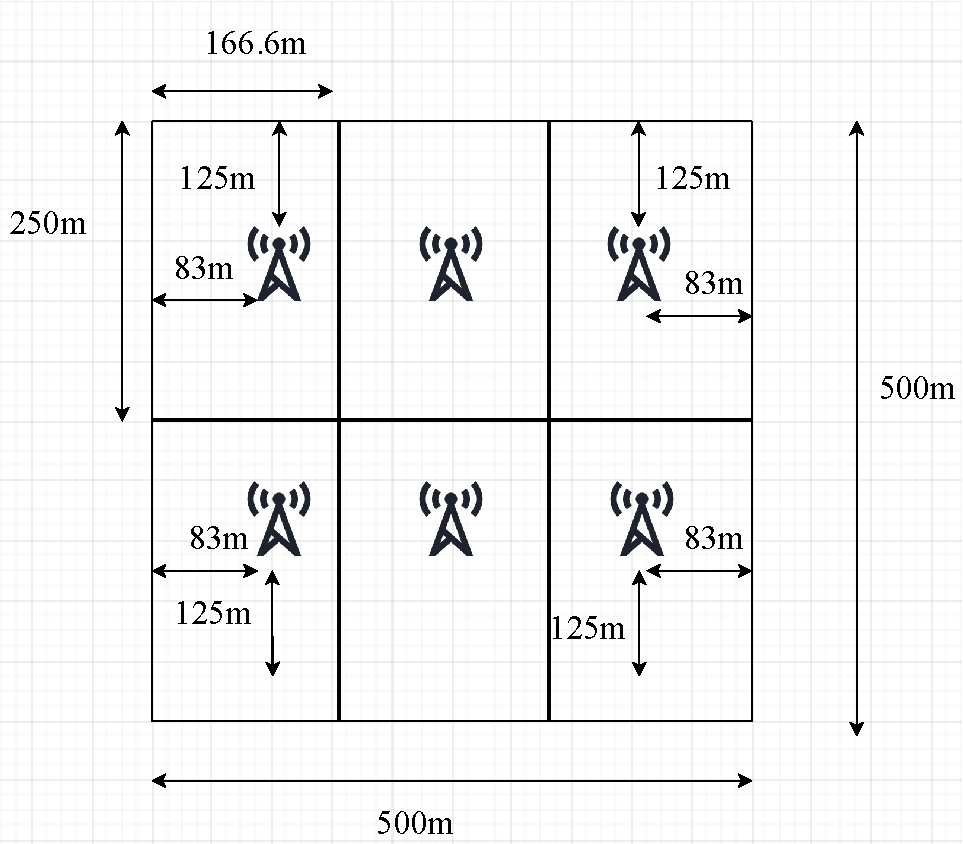
\includegraphics[scale = 0.30]{cell.pdf}
    %\includegraphics[max height=30cm,max width=9.5cm]{Drawing15.eps}
    %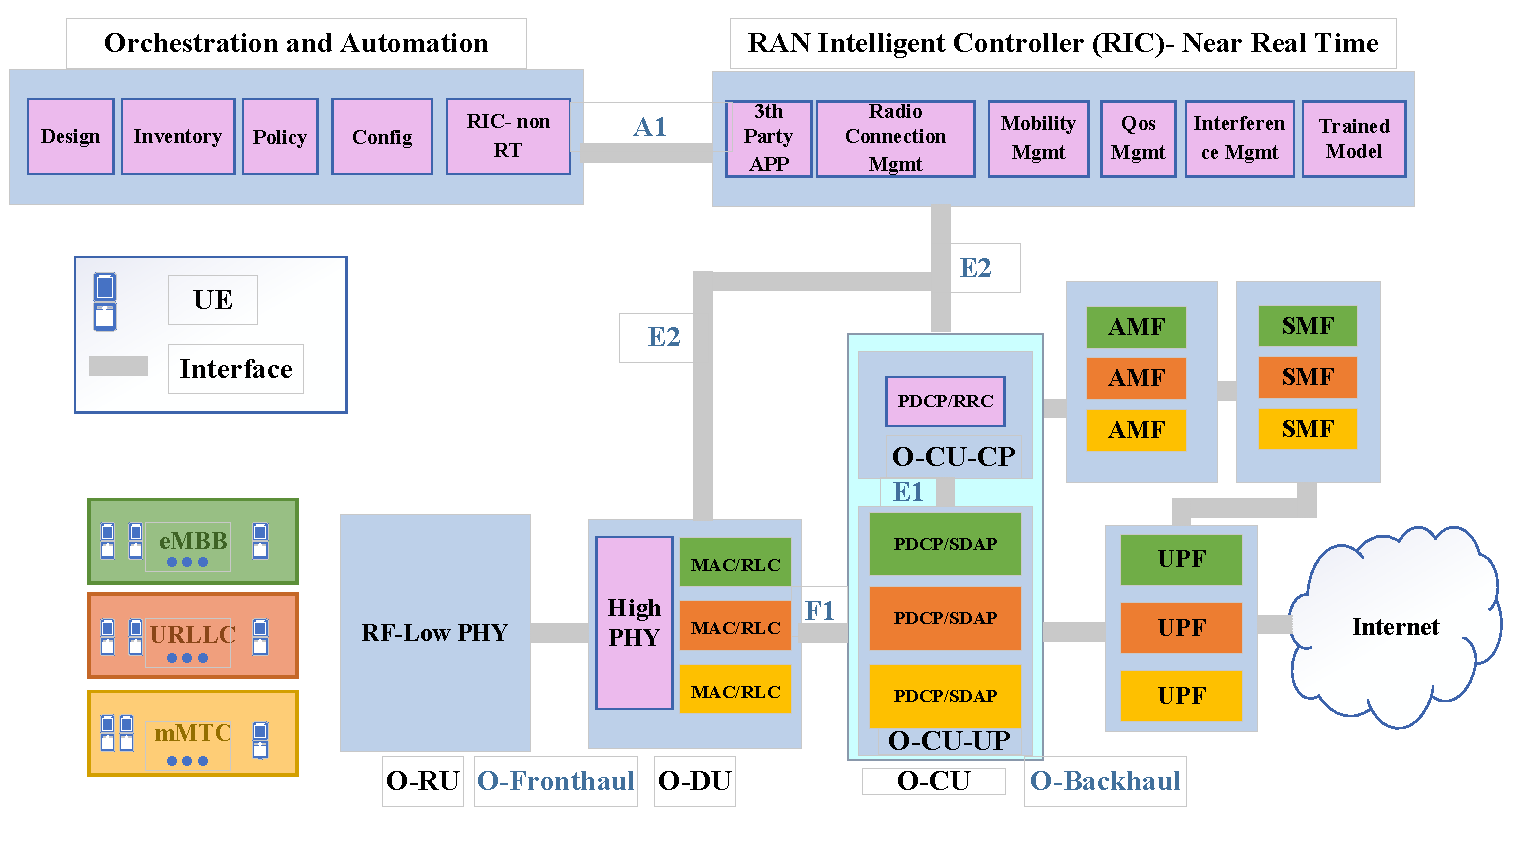
\includegraphics[width=\textwidth]{finalDraw.pdf}
  \caption{O-RU placement in a cell}
  \label{fig:cell}
\end{figure}

Here, the channel vector from the O-RU $r$ to the UE $i$ in service $s$ is set as $\bold{h}_{r,u(s,i)}^{k}=d_{r,u(s,i)}^{-\mathcal{L}} \Omega_{r,u(s,i)}^{k} $, where $d_{r,u(s,i)}^{-\mathcal{L}} $ is the distance between the O-RU $r$ and UE $i$ in service $s$ and $\mathcal{L} = 3.8$ is the path-loss exponent.% \cite{gholipoor2020cloud}.
Also, $\Omega_{r,u(s,i)}^{k}$ is the random variable that is generated by the Rayleigh distribution and it is the Rayleigh fading channel between the UE and O-RU.
We consider 25 PRBs in the network. The packet size for mMTC is equal to 20 bytes, and for URLLC is equal to 32 bytes \cite{ETSI1}.
The maximum number of VNF for each slice is 25 and the mean arrival data rate for the eMBB service is $\lambda  = 3Mbps$ and for the mMTC service and the URLLC  service is $\lambda  = 0.2Mbps$.
Also, the quantization noise is assumed to be $10^{-13}$.
Moreover, we set $\mathfrak{h}_{u_{(s,i)}} = \eta_{u_{(s,i)}}/200$, $\mathfrak{m}_{r} = \zeta_r/10$
and $\mathfrak{q}^k_{r,u(s,i)} = P_{s}^{max}/100$. The other parameters of these simulations are depicted in Table \ref{table:1a} \cite{3GPPTS1, 3GPPTS2,IMT, ETSI1}.%\cite{3GPPTS1, 3GPPTS2, 3GPPTS3, IMT, ETSI1}.


Finding a feasible initial value is almost tricky. We use a fast method discussed in \ref{fr} to overcome this challenge. 
Two different methods are used to compare the performance of the proposed method (IABV) and show the optimality of our approach.
The first one is a baseline scheme, which uses random PRB allocation. Therefore, the allocation of PRB to each UE is random when we have low interference, but in figures with high interference, we randomly assign just one RB to each UE. Also, the association of O-RU is carried out based on distance. It means that each UE is assigned to the nearest O-RU. The optimal power is obtained using the CVX of Matlab, which uses the successive convex approximation (SCA) method since the problem is convex.
After achieving power and other parameters, the achievable rate will be obtained, and the optimal number of VNF is achieved from Lemma \eqref{lemma1}.
\begin{table}%[H]
 \caption {Simulation Parameters} \label{table:1a}
 \begin{center}
 \scalebox{0.9}{
  \begin{tabular}{l  l }
  \toprule
\textbf{Parameter} & \textbf{Value} \\ [0.5ex]
  \toprule\toprule
  noise power & -174 dBm\\

  bandwidth & 180 KHz  \\

 maximum transmit power of each O-RU & 40 dBm \\

  maximum delay for eMBB &  4 msec \\

    maximum delay for URLLC &  1 msec \\

  maximum delay for mMTC &  5 msec \\

  maximum fronthaul capacity  & 46 bps \\

  minimum data rate for eMBB &  20 bps \\

   minimum data rate for URLLC and mMTC &  2 bps \\

   maximum received power for mMTC &  20 dBm \\ [.5ex]

    maximum received power for eMBB and URLLC &  33 dBm \\ [.5ex]
 \toprule
 \end{tabular}}
 \vspace*{-1.em}
 \end{center}
 \end{table}
For the second one, we use the idea of the fixed BBU capacity and dynamic resource allocation (FBDR) algorithm proposed in \cite{lee2018dynamic} and named it the dynamic resource allocation scheme (DR scheme). 
 We have services with different QoS in this work, similar to tenants with different QoS introduced in \cite{lee2018dynamic}. Therefore, we can use the DR scheme similar to the FBDR method adapted to our conditions for comparison. Instead of BBU in C-RAN, we have O-DU and O-CU in O-RAN.
 Since we do not talk about O-DU and O-CU capacity, we use the dynamic resource allocation scheme (DR scheme) algorithm and do not consider BBU capacity.
 In the DR scheme, PRB and power are dynamically allocated. The number of VNFs is obtained from the simulation. The UEs are associated with the O-RU based on the quality of their channels and the channel distance instead of using the greedy algorithm \ref{alg1} (GAA algorithm) for O-RU assignment. The figures in \cite{lee2018dynamic} show that dynamic BBU capacity and dynamic resource allocation (DBDR) perform better than FBDR for the same priority area. The numerical results section also indicates that our proposed algorithm performs better than the DR scheme.
\vspace*{-0.9em}
\subsection{Feasible Region}\label{fr}
Applying the correct initial point is crucial in making the system feasible and convergent.
Therefore, we investigated the non-converging and converging simulation for models with fixed initial parameters and UE random channel gains.
We experimentally found that in non-converged simulations, there are UEs at the edge of the boundaries or far away from the O-RU and have a weak channel gain. One solution is to eliminate UEs who undermine system convergence.
For a large number of UEs with a fixed number of PRBs, the probability of having an infeasible solution increases due to a large number of UE interference.
Another solution is to remove the simulations in the Monte-Carlo that do not converge using the fast algorithm (FA) to check the convergence before
the proposed algorithm (IABV).
Therefore, if more than half of the iterations have a feasible solution for the initial condition, the simulation can be displayed as a feasible model.
If the conditions in \eqref{RConstr}, \eqref{pr11}, \eqref{c12-1} and \eqref{c12} are met in the fast algorithm (FA), the given algorithm will converge.
Assume, the number of UEs is $\mathfrak{N} = \sum_{s=1}^{S}\sum_{i=1}^{U_s}1$,
the number of PRBs is $K$, and the distance between the $r^{th}$ O-RU to the UE i in slice $s$ is $d_{r,u(s,i)}$.
The FA algorithm is represented in Algorithm \ref{alg3}.
The complexity order of this algorithm is $O(R\times \mathfrak{N})$ which is remarkably lower than the complexity order of the IABV method.
In the FA algorithm, the O-RU association is based on the distance of the UE to the O-RU.
Each UE is associated with the nearest O-RU. Also, the power of each UE is set to be the minimum of the maximum power of each UE and the maximum power of each O-RU divided by the total number of UEs ($\min\{P_s^{\max}, P_r^{\max}/\mathfrak{N}\}$).
Moreover, the allocation of PRBs to UEs is based on dividing the number of UEs by the total number of PRBs.
\vspace*{-1.em}
\subsection{Numerical Results}
In Fig. 3, the aggregate throughput is demonstrated versus the different number of UEs in each service for these three methods. Suppose we have one service instance for each type of service, so we have three various services in this figure. Also, we have between 6 to 48 UEs in the system.
Here, we did not consider the priority. The figure presented that the proposed method, IABV, is $18.6\%$ higher throughput than the baseline scheme.
As the number of UEs increases in each service, the aggregated throughput initially increases. Still, due to the interference and the power constraint, it will be saturated from 12 UEs in each service.


\begin{figure*}[!htb]
	\centerline{%
		\begin{tabular}{c@{}c@{}c}			
			\includegraphics[scale = 0.4]{fig/Arate_ue1_1n.eps} &
			\includegraphics[scale = 0.4]{fig/vnfNum1n.eps} &
			\includegraphics[scale = 0.4]{fig/RatePower1n.eps} \\
			\scriptsize Fig. 3~Aggr. throughput vs. number of UEs in each service & \scriptsize  Fig. 4~Number of VNFs in each service vs. arrival rate & \scriptsize Fig. 5~Aggr. throughput for eMBB vs. maximum  power 
	\end{tabular}}
	%\caption{Global caption.}
	\label{label}
\end{figure*}

Fig. 4 depicts the number of activated VNFs for five different mean service times of one URLLC service vs. the mean arrival time for 12 UEs. This figure presents that as the mean arrival rate increases, the number of activated VNF increases. Moreover, the number of activated VNFs decreases when the mean service rate increases.


In Fig. 5, the aggregate throughput is depicted vs. the maximum power of UE for three different instances of eMBB service using proposed method (IABV), DR scheme and the baseline scheme. Here, we suppose that we have 12 UEs in each service.  We assume that these three services require 5bits/sec/Hz, 10bits/sec/Hz, and 15bits/sec/Hz.
%In addition, We suppose that each O-RU can transmit three times of the maximum power of the UEs.
As you can see in the figure, increasing the maximum power increases the aggregate throughput. Moreover, the proposed method (IABV), gives higher aggregate rates in compared to the DR scheme and the baseline scheme.

\begin{figure*}[!htb]
	\centerline{%
		\begin{tabular}{c@{}c@{}c}			
			\includegraphics[scale = 0.4]{fig/delay_newn.eps} &
			\includegraphics[scale = 0.4]{fig/delay1_newn.eps} &
			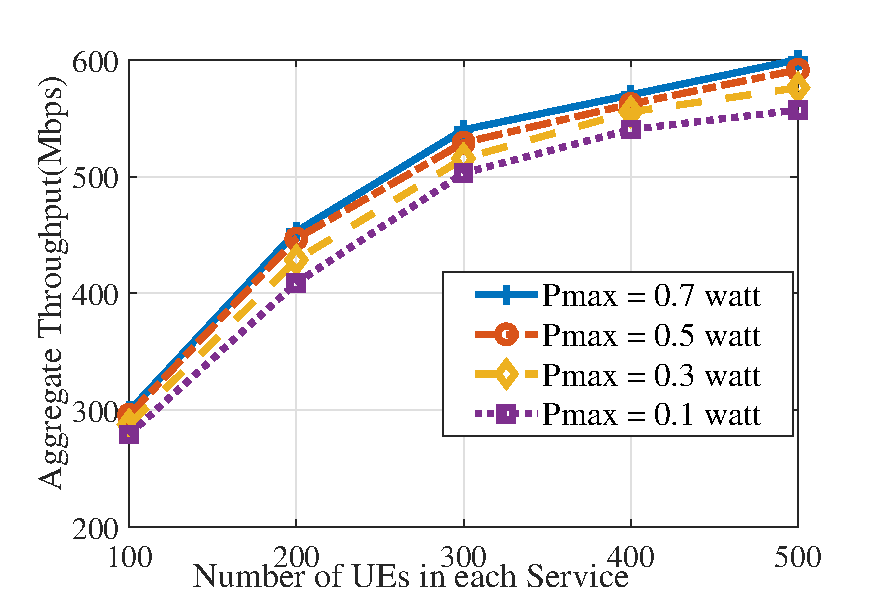
\includegraphics[scale = 0.4]{fig/AmmTCpowern.eps} \\
			\scriptsize Fig. 6~~Total Delay of a URLLC vs. the arrival rate of a UE  & \scriptsize Fig. 7~~ Total Delay of a URLLC vs. arrival rate of a UE  & \scriptsize Fig. 8~~Aggr. throughput vs. the number of mMTC UEs
	\end{tabular}}
	%\caption{Global caption.}
	\label{label}
\end{figure*}

%%%%%%%%%%%%%%%%%%%%
Fig. 6 illustrates the mean total delay of a UE in a URLLC service regarding the mean arrival rate of the UE and the number of UEs in the service for the proposed method (IABV).
It is shown that the delay is an ascending function of the mean arrival rate (when the mean service time is fixed) and the number of UEs in the service.
% In this figure, we assume that the maximum number of VNF for each slice is 50 and the maximum delay of each UE in a URLLC service is $0.5ms$. 
%Also, the maximum number of PRB is considered to be 50.
 Moreover, we can see that the mean delay of a URLLC service
does not reach the maximum threshold of the delay.

%Moreover, we can see that the mean delay of a URLLC service increases almost linearly with the mean arrival rate of the packet transmission.
%%%%%%%%%%%%%%%%%
%\begin{figure}
%  \centering
%    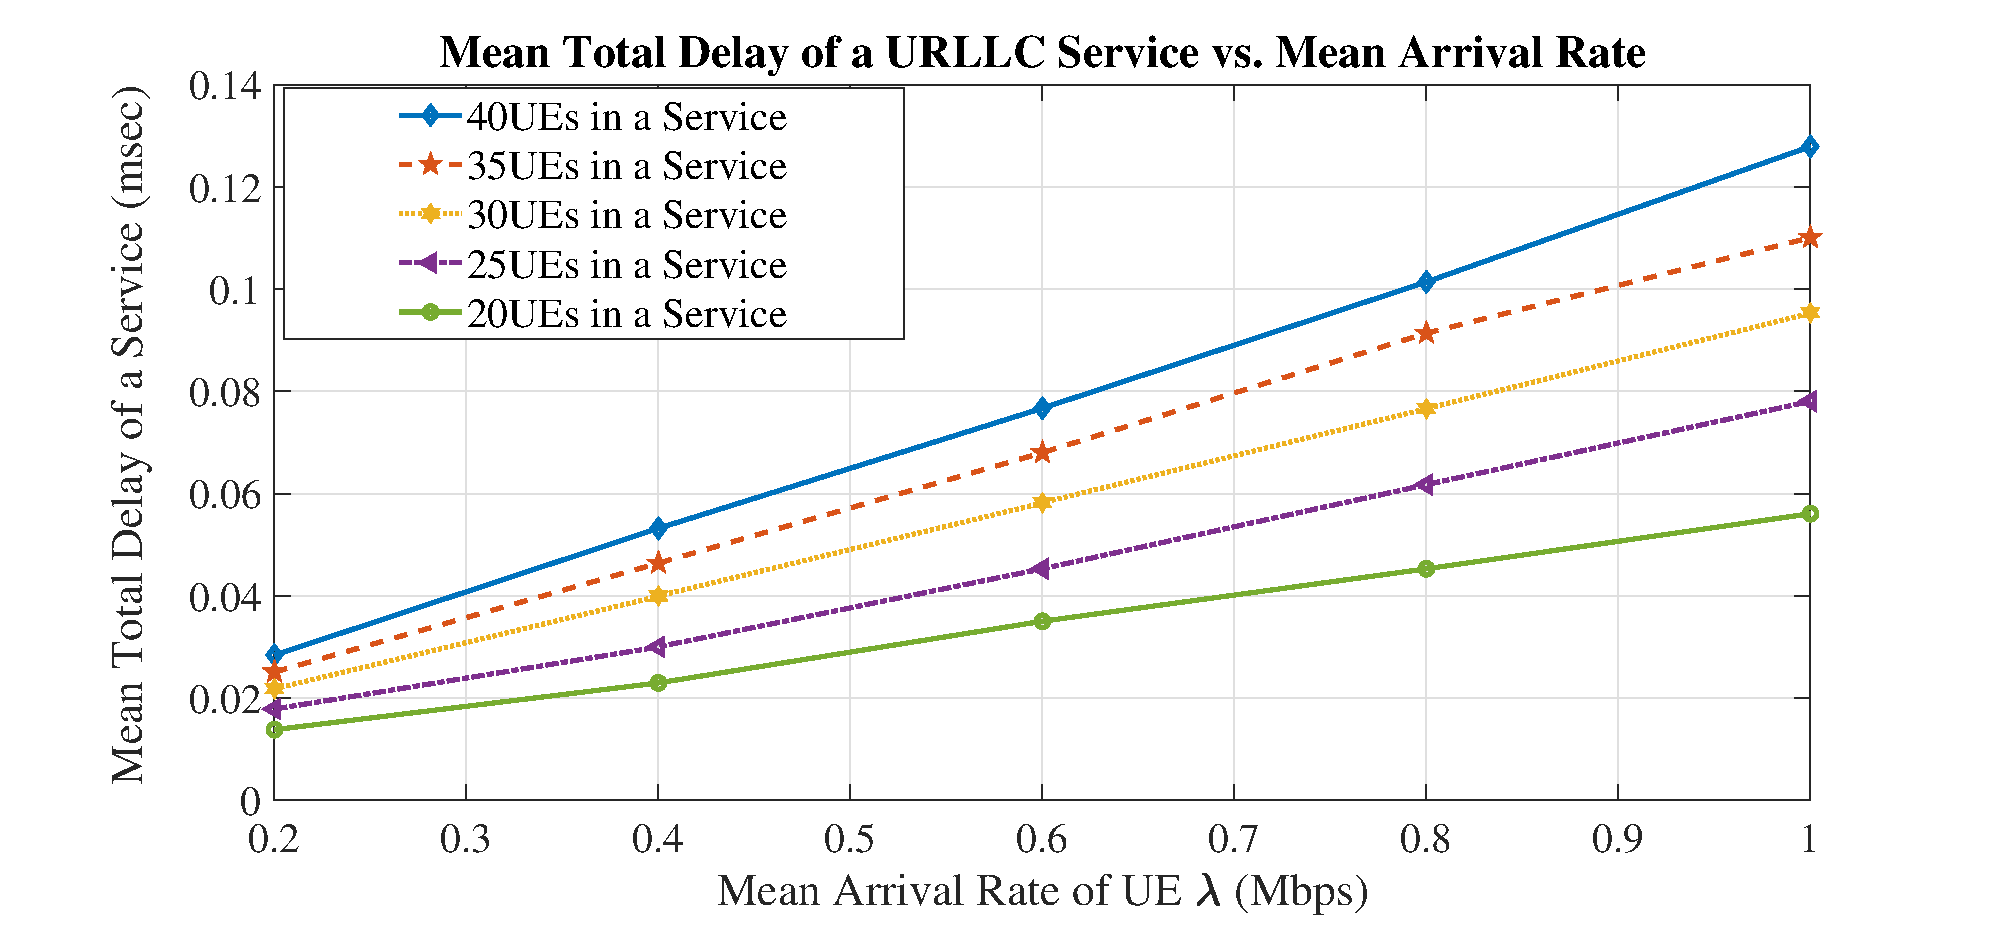
\includegraphics[scale = 0.47]{delay_new.eps}
%    %\includegraphics[max height=30cm,max width=9.5cm]{Drawing15.eps}
%    %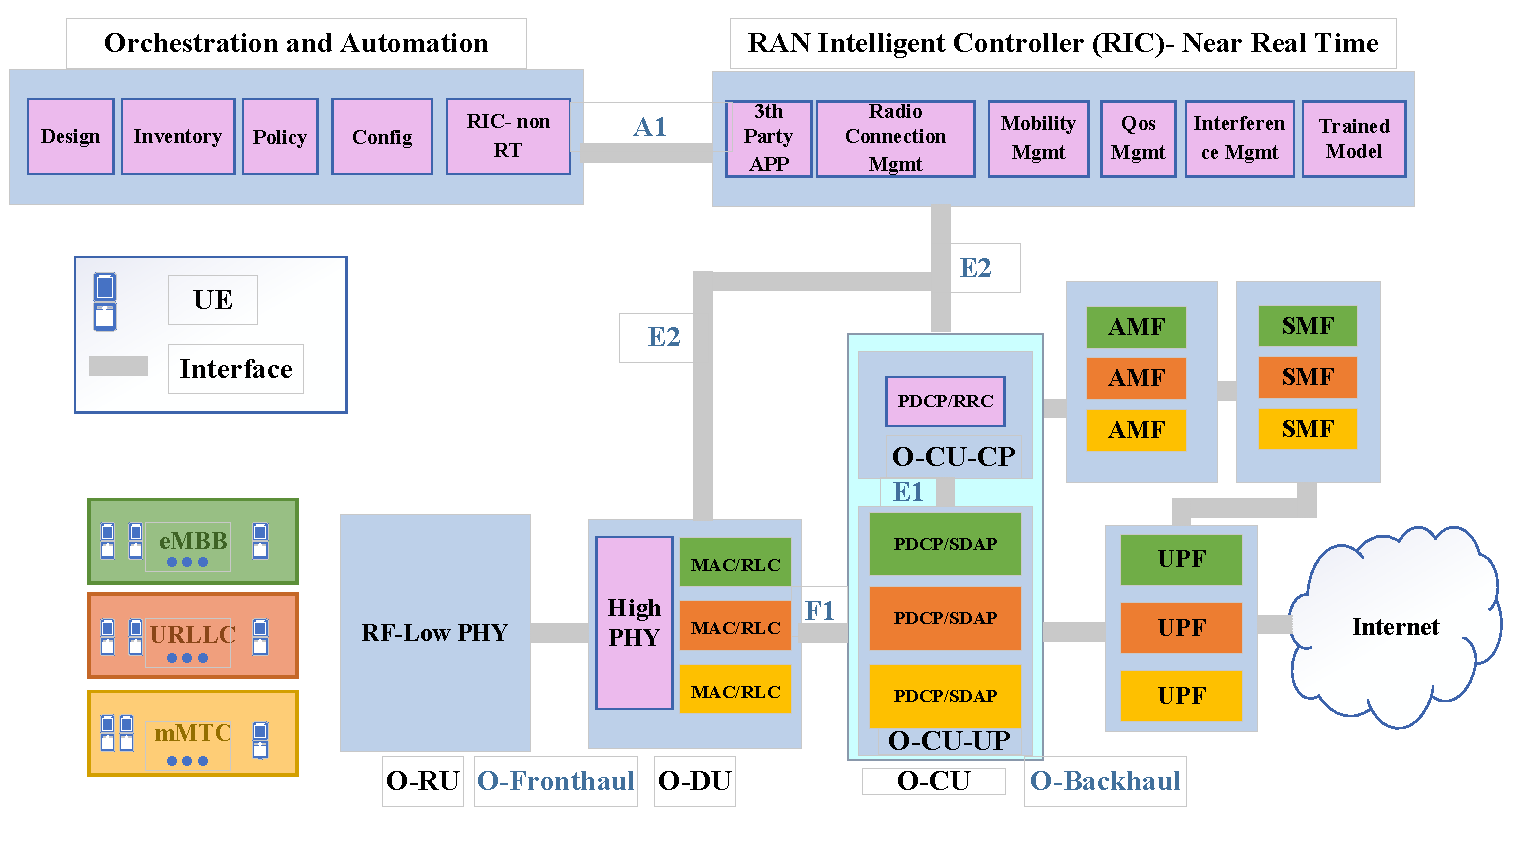
\includegraphics[width=\textwidth]{finalDraw.pdf}
%  \caption{Mean Total Delay of a URLLC Service vs. the Mean Arrival Rate of a UE in the Service for various number of UEs}
%  \label{fig:6}
%\end{figure}
%%%%%%%%%%%%%%%%%%%%5
Fig. 7 is the same as Fig. 6 that presented the mean total delay of a UE in a URLLC service regarding the mean arrival rate of the UE for 20 UEs using three different methods. As you can see, the proposed method (IABV) outperforms the other scenarios.

Fig. 8, represents the aggregate throughput concerning the number of UEs in each service and the maximum power for three different mMTC service instances. 
Assume each UE in each mMTC service instance requires 0.1 bits/sec/Hz data rate and is not sensitive to the end-to-end delay. There is no restriction on fronthaul link capacity and the number of VNFs.
%Moreover, to make the simulation feasible, we assume that the number of PRBs is as large as the system has low interference.
%so we suppose there is a fixed  PRB allocation in the simulation that each UE is allocated to one PRB. There is no PRB with more than one UE allocation.
The figure depicts that by increasing the number of UEs in each instance of the service, or by increasing the maximum power of each UE in each instance of mMTC service, the aggregate throughput increases.
%Also, by increasing the maximum power of each UE in each instance of mMTC service, the aggregate throughput rises too.

%%%%%%%%%%%%
%\begin{figure}
%  \centering
%    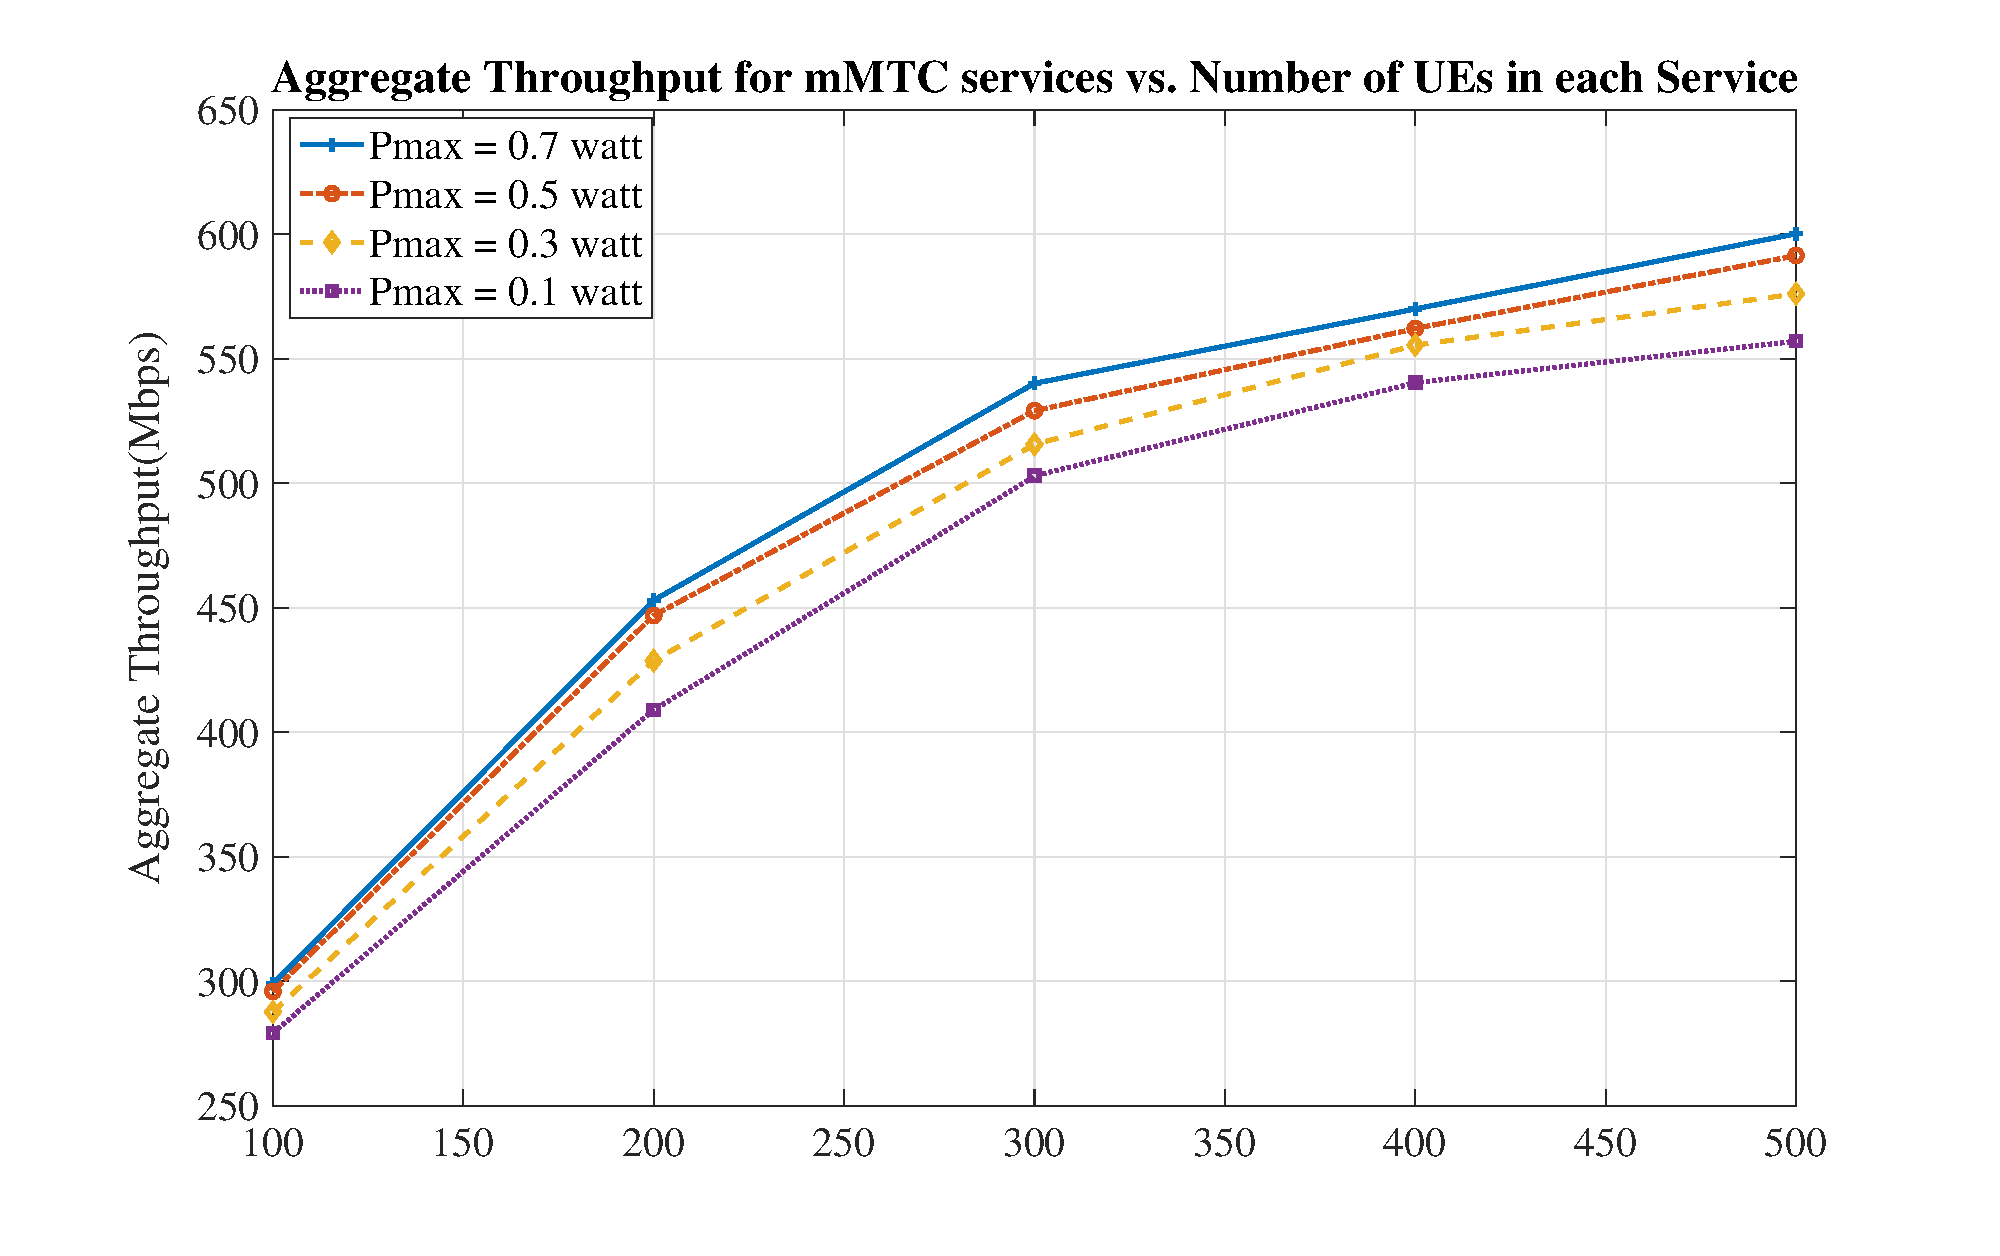
\includegraphics[scale = 0.4]{AmmTCpower.eps}
%    %\includegraphics[max height=30cm,max width=9.5cm]{Drawing15.eps}
%    %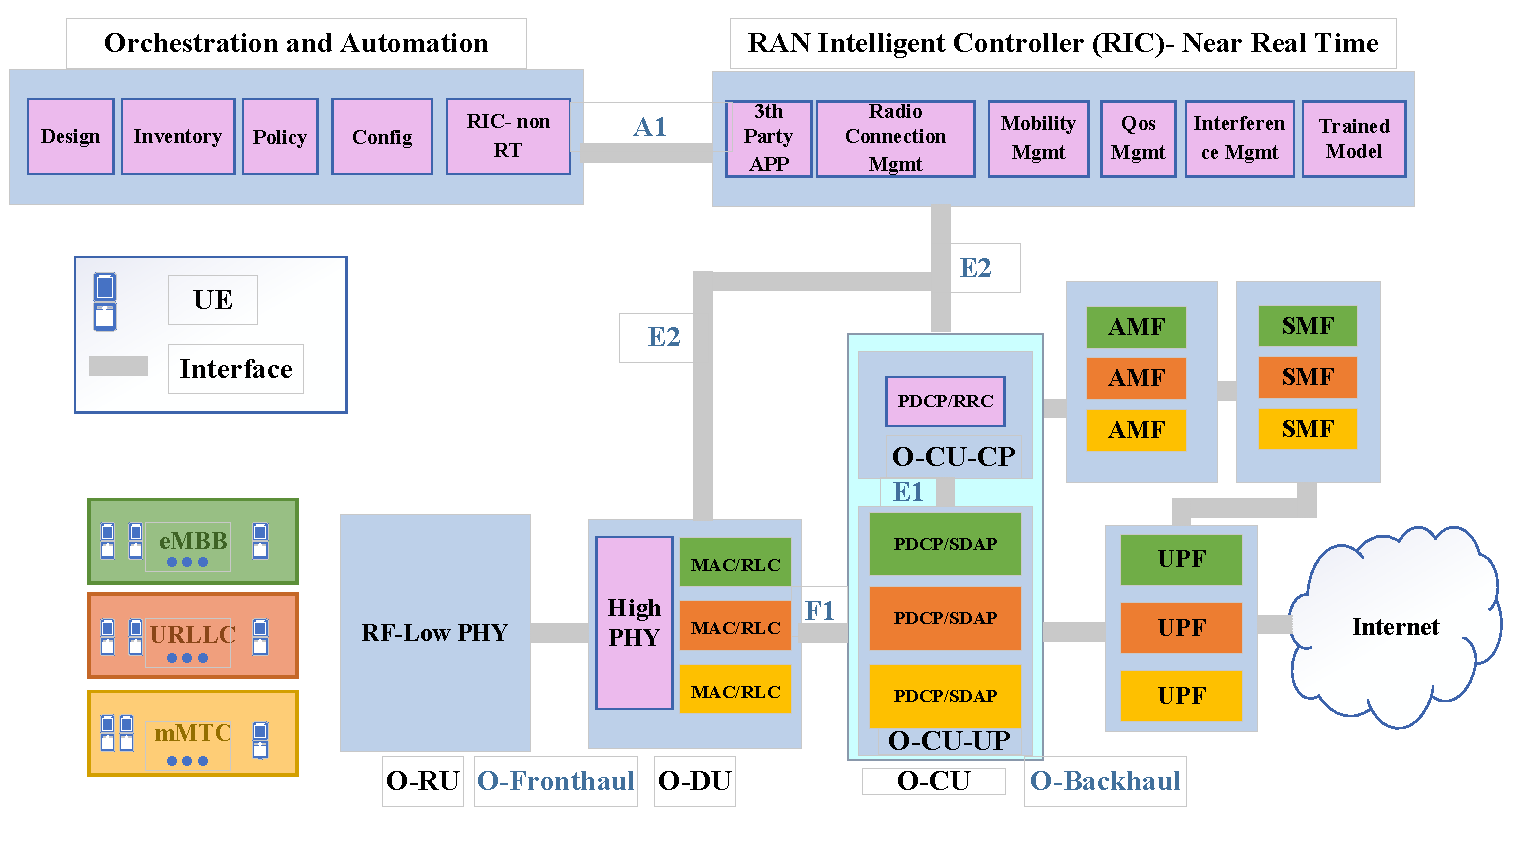
\includegraphics[width=\textwidth]{finalDraw.pdf}
%  \caption{Aggregate Throughput for mMTC services vs. Number of UEs in each Service for three different mMTC service instances}
%  \label{fig:8}
%\end{figure}
%%%%%%%%%%%%
Assume we have two types of eMBB service instances. In Fig. 9, the aggregate throughput (by considering the priority factor $\delta_s$) is depicted for two eMBB service instances. Here we consider 4 UEs in each service. %We assume that the the fronthaul link and the end-to-end delay have no restrictions.
The Fig. 9 presented that by increasing the priority factor for one service instance, more resources are allocated to this service instance, and the aggregate throughput of this service is increased and vice versa. Also, we can realize from this figure that the aggregate throughput has the most significant value at the same priority.

\begin{figure*}[!htb]
	\centerline{%
		\begin{tabular}{c@{}c@{}c}			
			\includegraphics[scale = 0.4]{fig/priorityLastn.eps} &
			\includegraphics[scale = 0.4]{fig/itern.eps} &
			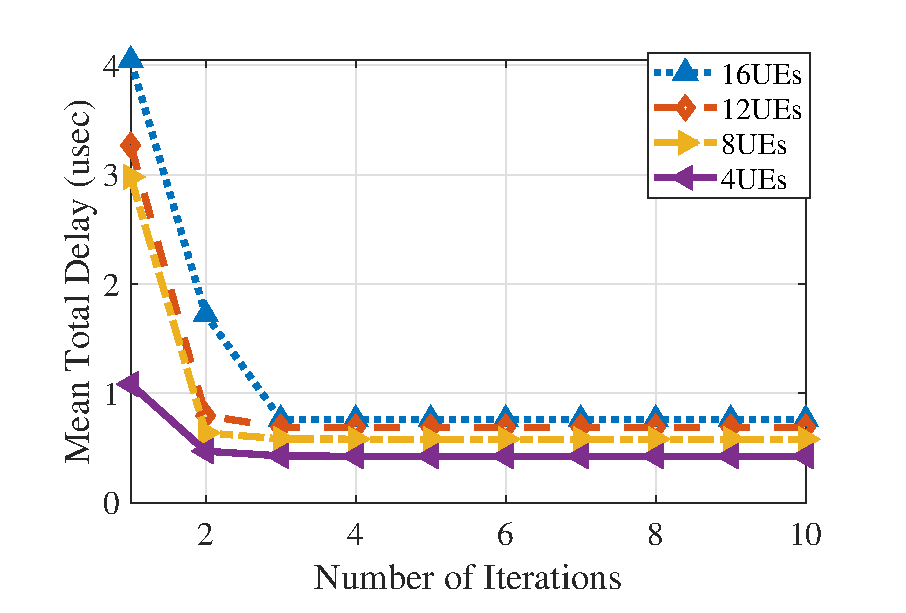
\includegraphics[scale = 0.4]{fig/iterD.eps} \\
			\scriptsize Fig. 9~~Throughput of eMBB services vs. priority of the first one  & \scriptsize Fig. 10~~Aggregate throughput vs. number of iterations  & \scriptsize Fig. 11~~Mean Delay time vs. number of iterations 
	\end{tabular}}
	%\caption{Global caption.}
	\label{label}
\end{figure*}

%%%%%%%%%%5
%\begin{figure}
%  \centering
%    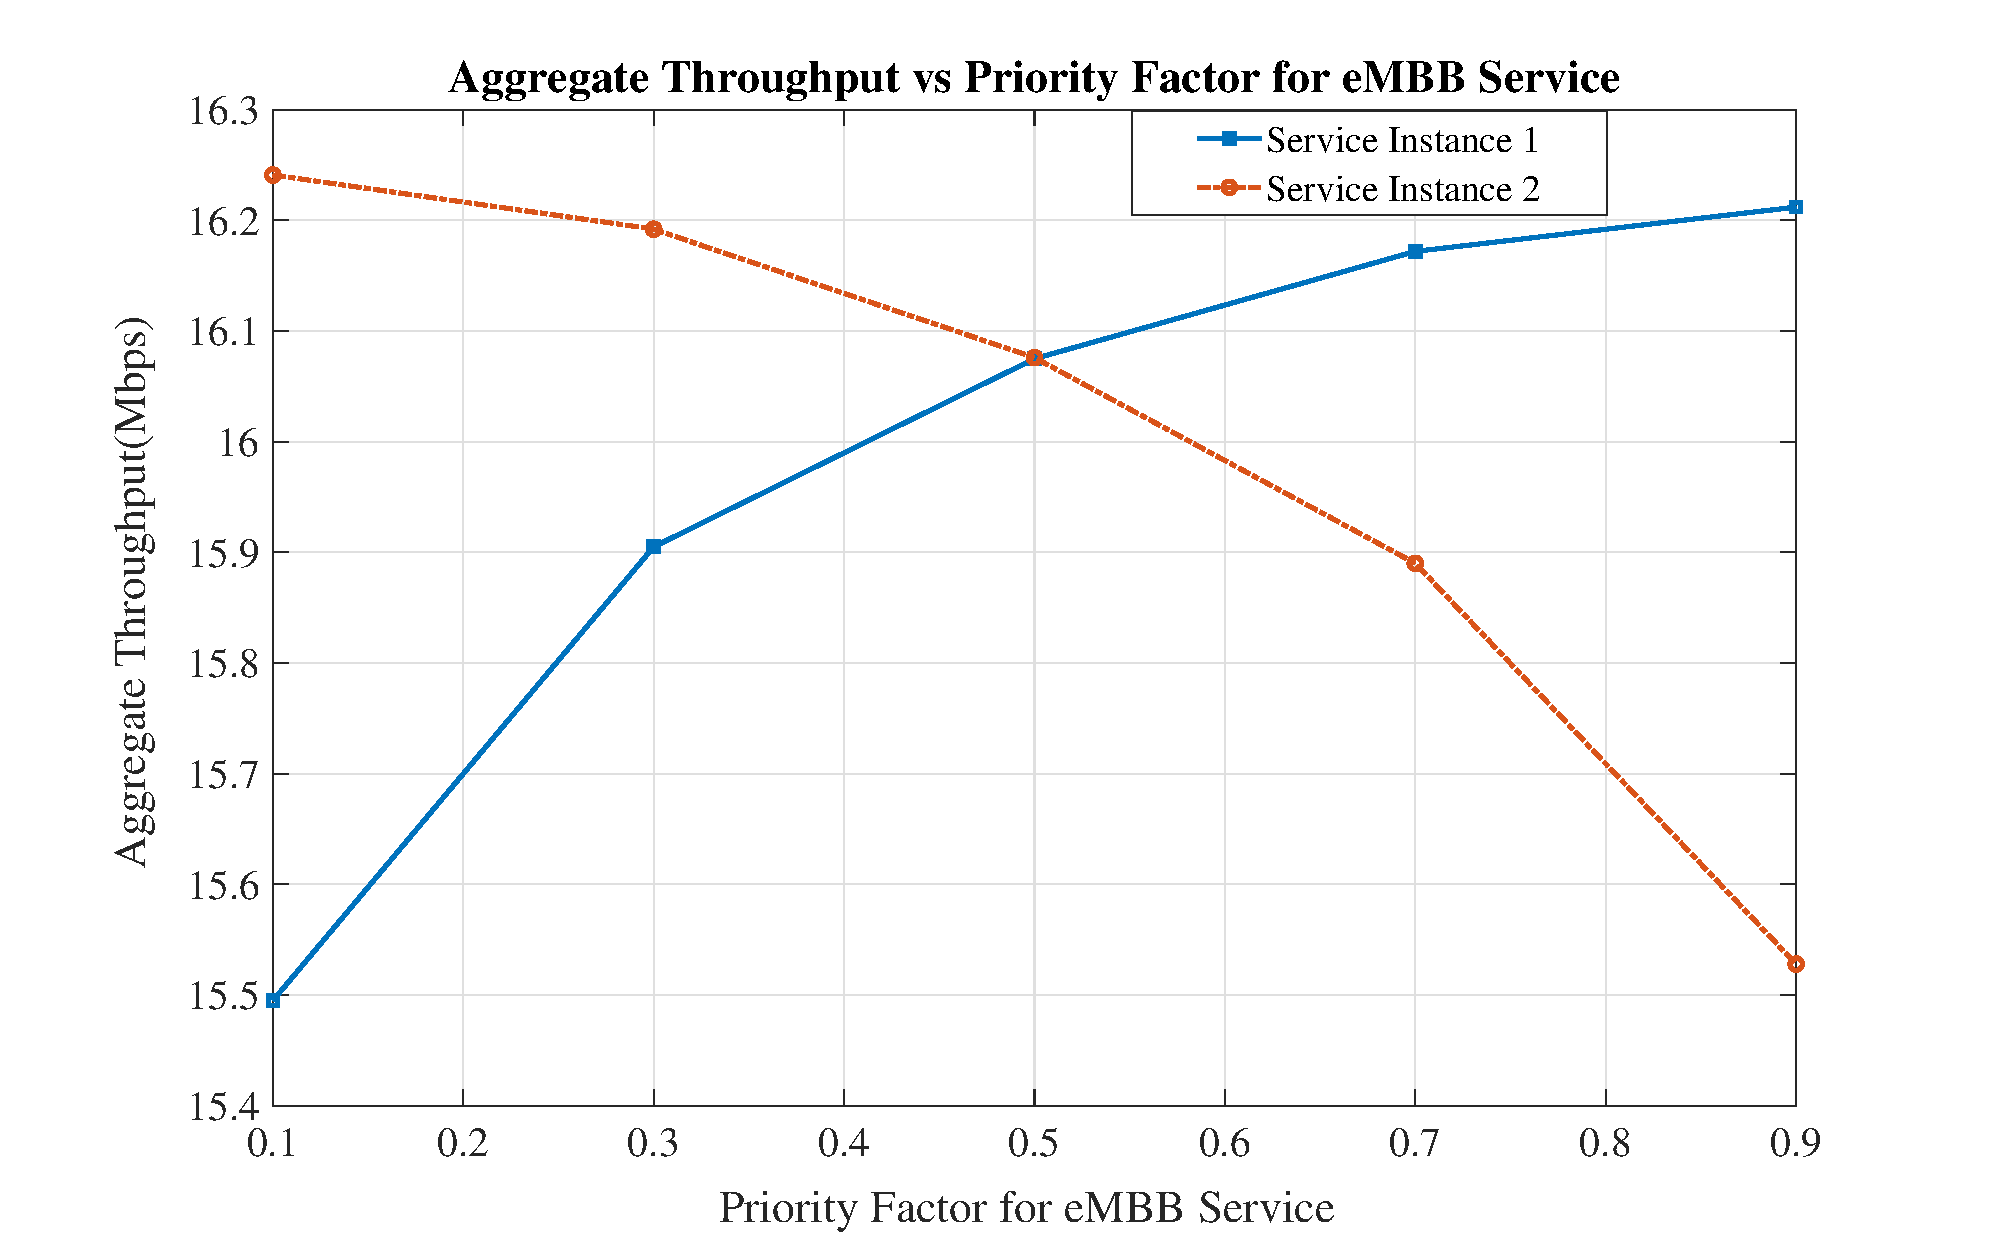
\includegraphics[scale = 0.4]{priorityLast.eps}
%  \caption{Aggregate Throughput for two eMBB service instances vs. Priority of the first service instance }
%  \label{fig:9}
%\end{figure}
%%%%%%%%%%%
%In the figure \ref{fig:10}, the aggregate throughput is presented vs. the number of UEs for one service in a system by considering two different cloud restrictions and fronthaul restrictions.
%In the graph of cloud restriction, we have the restrictions in O-DU and O-CU.
%In the graph of fronthaul restriction, we have the restrictions in O-RU.
%In the O-RU restriction graph, we assume that the fronhaul link is set to be 47 bits/sec/Hz (the variance of quantization noise is $10^{-13}$) , and the maximum power of each O-RU is 40 dBm. Also, the maximum power of each UE is set to be 35 dBm. Moreover, the minimum data rate for each UE in this service is 6 bits/sec/Hz. In this graph, we assume that there is less restriction in the end-to-end delay (50 ms) and the VNF resources (the system has 100 reserved VNF).
%In the graph of cloud restriction, we assume that there is no restriction on the fronthaul link.
%The limitation on the power is less than the graph of fronthaul limitation, and it is set to be 45 dBm on the power of each O-RU, and the maximum power of each UE is 40 dBm.
%The minimum data rate for each UE in this service is 10 bits/sec/Hz.
%The end-to-end delay for each UE is 4ms and the mean arrival rate is 2Mbps.
%and the mean service rate is 10Mbps.
%In this figure, the consequence of cloud limitation and fronthaul limitation is depicted.
%As the number of UEs increases, the aggregate throughput rises linearly, and the graph of cloud restriction increases more than the other graph of fronthaul limitation.

%\begin{figure}
%  \centering
%    \includegraphics[scale = 0.4]{AcloudVsFronthaul.eps}
%    %\includegraphics[max height=30cm,max width=9.5cm]{Drawing15.eps}
%    %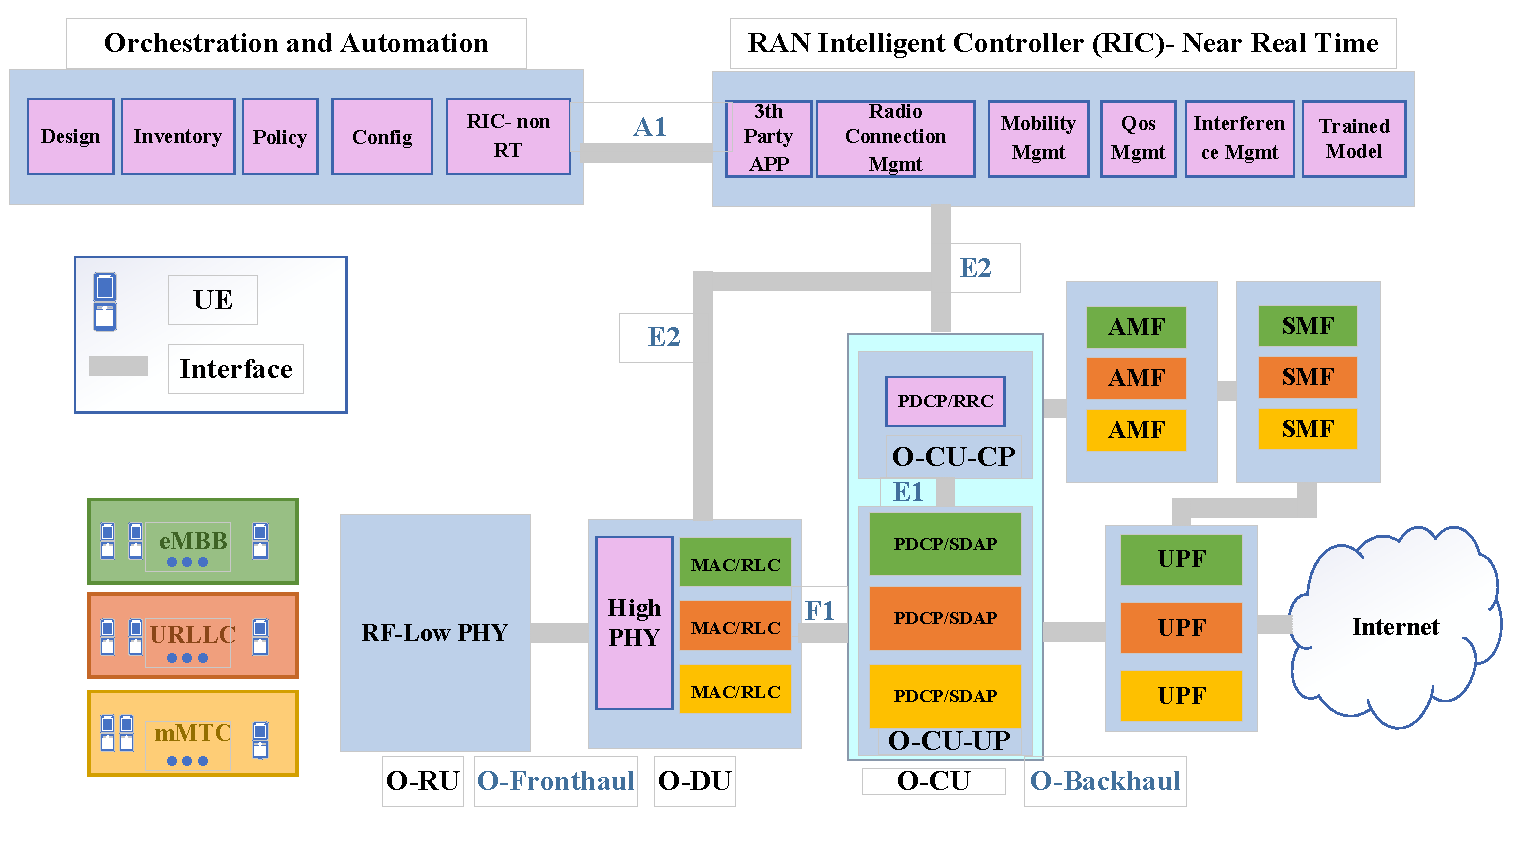
\includegraphics[width=\textwidth]{finalDraw.pdf}
%  \caption{Aggregate Throughput vs. Number of UEs in a Service}
%  \label{fig:10}
%\end{figure}
In Fig. 10, the aggregate throughput is shown according to the number of iteration (outer loop) of the
proposed algorithm (IABV) for different numbers of UEs for one service. In this figure, the convergence of the IABV method is illustrated. The minimum data rate for each UE is assumed to be 2 Mbps.
After four iterations, IABV converges to the fixed value.

In Fig. 11, the mean total delay of URLLC service is indicated according to the number of iterations of the
proposed algorithm (IABV) for different numbers of UEs for one URLLC service. This figure shows that the algorithm converged to the fixed value after four iterations.

%%%%%%%%%%%%%%%%%%%%%%%%%55
%\begin{figure}
%  \centering
%    \includegraphics[scale = 0.4]{iter.eps}
%    %\includegraphics[max height=30cm,max width=9.5cm]{Drawing15.eps}
%    %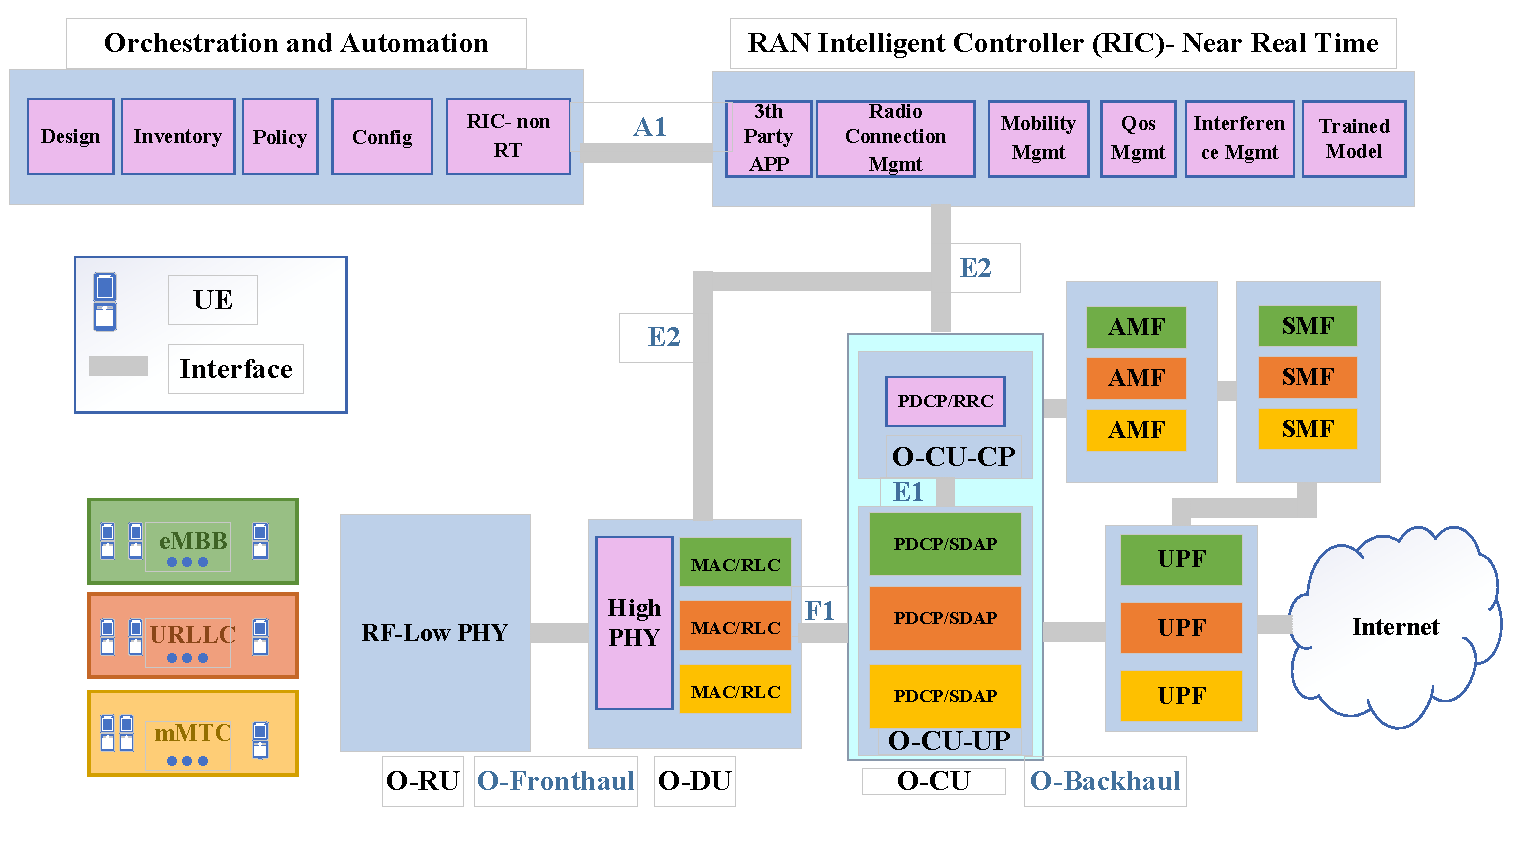
\includegraphics[width=\textwidth]{finalDraw.pdf}
%  \caption{Aggregate Throughput vs. Number of Iterations}
%  \label{fig:11}
%\end{figure}
%%%%%%%%%%%%%%%%%5
%\subsection{Summary of Simulation Results}
In Fig. 12, the aggregate throughput is shown according to the number of UEs for two different methods, namely the
proposed algorithm (IABV) and the optimal method for URLLC service for the low interference.
The minimum data rate is 5bits/sec/Hz for each UE and the maximum delay is $0.1$ms.
Also the mean arrival rate is set to be $0.2$Mbps and the mean service rate is $0.5$Mbps.
%The other parameters are depicted in Table \ref{table:1a}.
The optimal approach is obtained from the two-step joint exhaustive search and using CVX.
In each iteration in the first step, the PRB allocation and O-RU association are obtained from brute force, and in the second step, we use CVX to get optimal power.
Our solution is close to the optimal value in a small number of UEs.


\begin{figure*}[!htb]
	\centerline{%
		\begin{tabular}{c@{}c@{}c}			
			\includegraphics[scale = 0.4]{fig/optimal1n.eps} &
			\includegraphics[scale = 0.4]{fig/interF_newn.eps} &
			\includegraphics[scale = 0.4]{fig/FAn.eps} \\
			\scriptsize Fig. 12~~Aggregate throughput vs. number of UEs   & \scriptsize Fig. 13~~Aggregate throughput vs. maximum interference   & \scriptsize Fig. 14~~Aggregate throughput vs. number of UEs
	\end{tabular}}
	%\caption{Global caption.}
	\label{label}
\end{figure*}
%\begin{figure}
%  \centering
%    \includegraphics[scale = 0.4]{optimal1.eps}
%    %\includegraphics[max height=30cm,max width=9.5cm]{Drawing15.eps}
%    %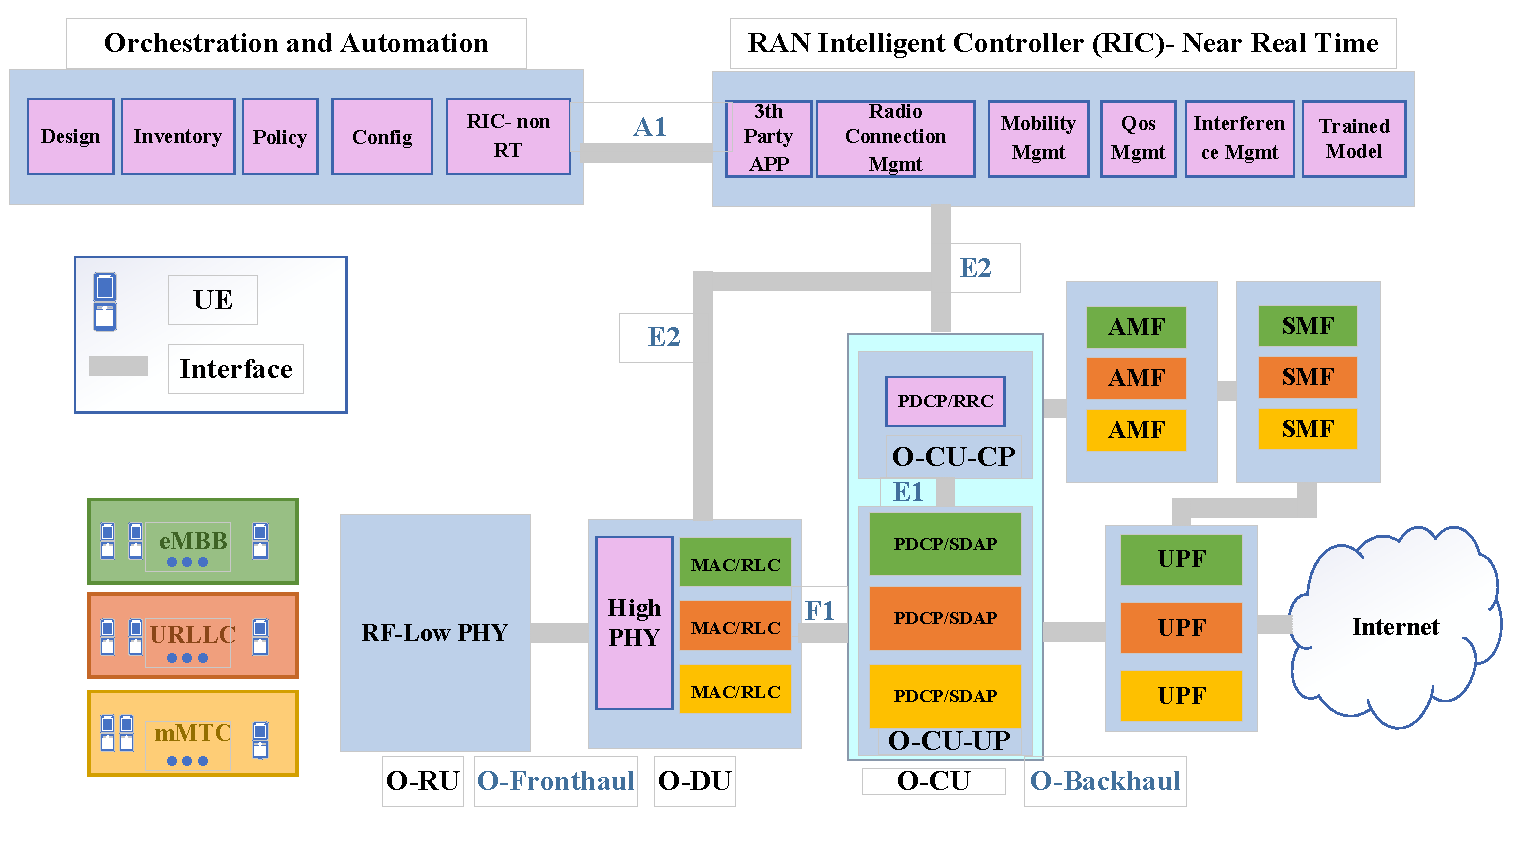
\includegraphics[width=\textwidth]{finalDraw.pdf}
%  \caption{Aggregate Throughput vs. Number of UEs }
%  \label{fig:12}
%\end{figure}

In Fig. 13, the aggregate throughput is depicted vs. the maximum interference for two different maximum power thresholds of O-RU. 
%We suppose that the maximum power threshold of UEs is one-third of the maximum power of O-RU.
%The minimum data bit rate is assumed to be 0.2Mbps for each UE.
Here we assume that with the increase of every ten dBm of interference power, it is assumed that ten users have been added to the system. In -105 dBm, we have 5 UEs, and at the end, we have 55 UEs in the system.
Since the amount of interference in the system is entered as a fixed value,
the allocation of PRBs is not considered.
The higher maximum power threshold leads to a greater aggregate throughput.
The aggregate throughput first increases with the number of UEs and at the same time the amount of the maximum interference, then it becomes almost fixed and finally decreases so much. When the aggregate throughput decreases, the maximum interference is so high that it takes the system out of feasibility.
%The aggregate throughput rises with the increases of UEs and the maximum interference and then remains almost constant.

%\begin{figure}
%  \centering
%    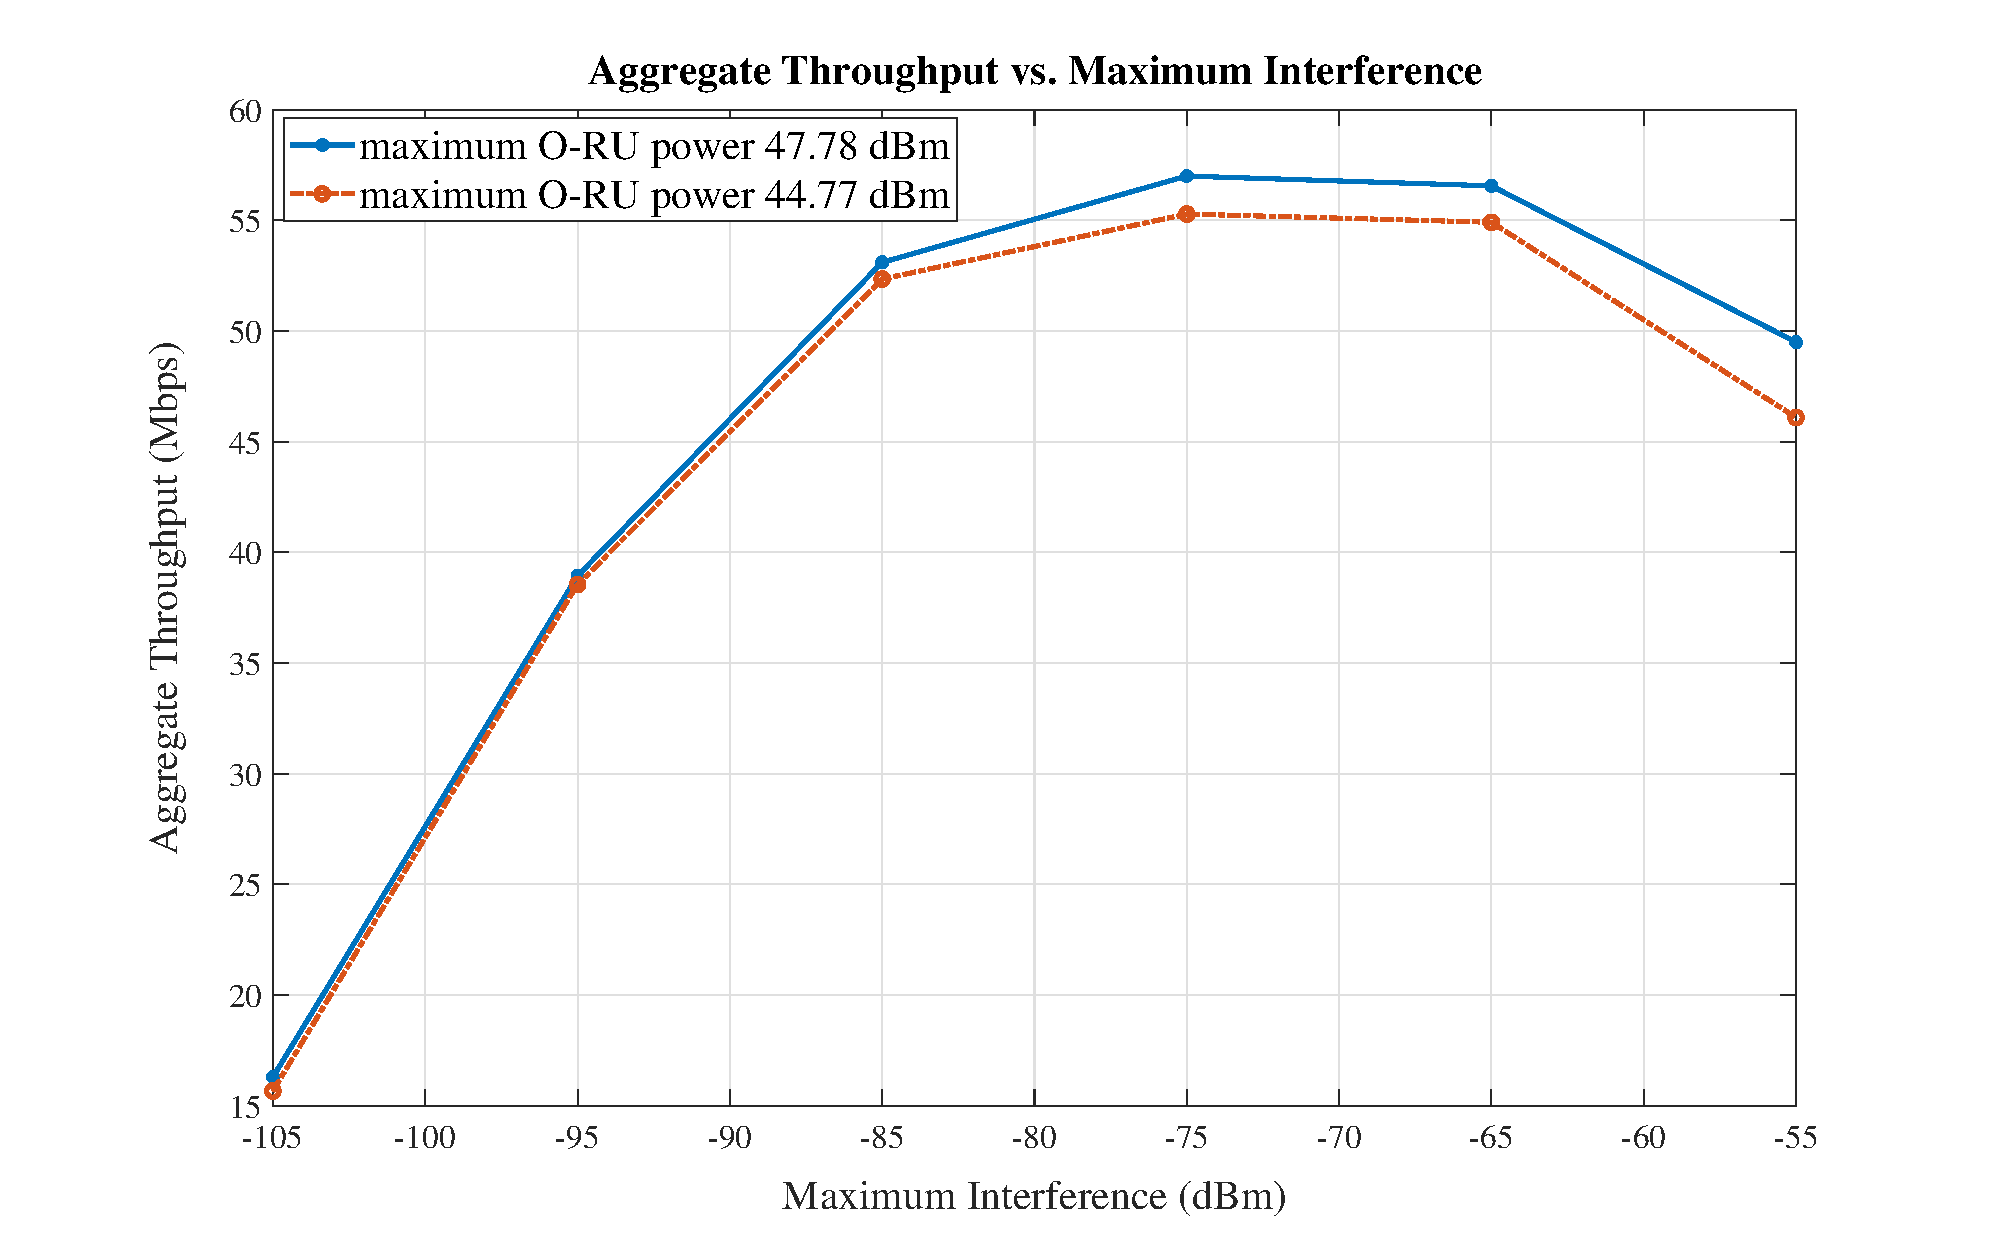
\includegraphics[scale = 0.4]{interF_new.eps}
%    %\includegraphics[max height=30cm,max width=9.5cm]{Drawing15.eps}
%    %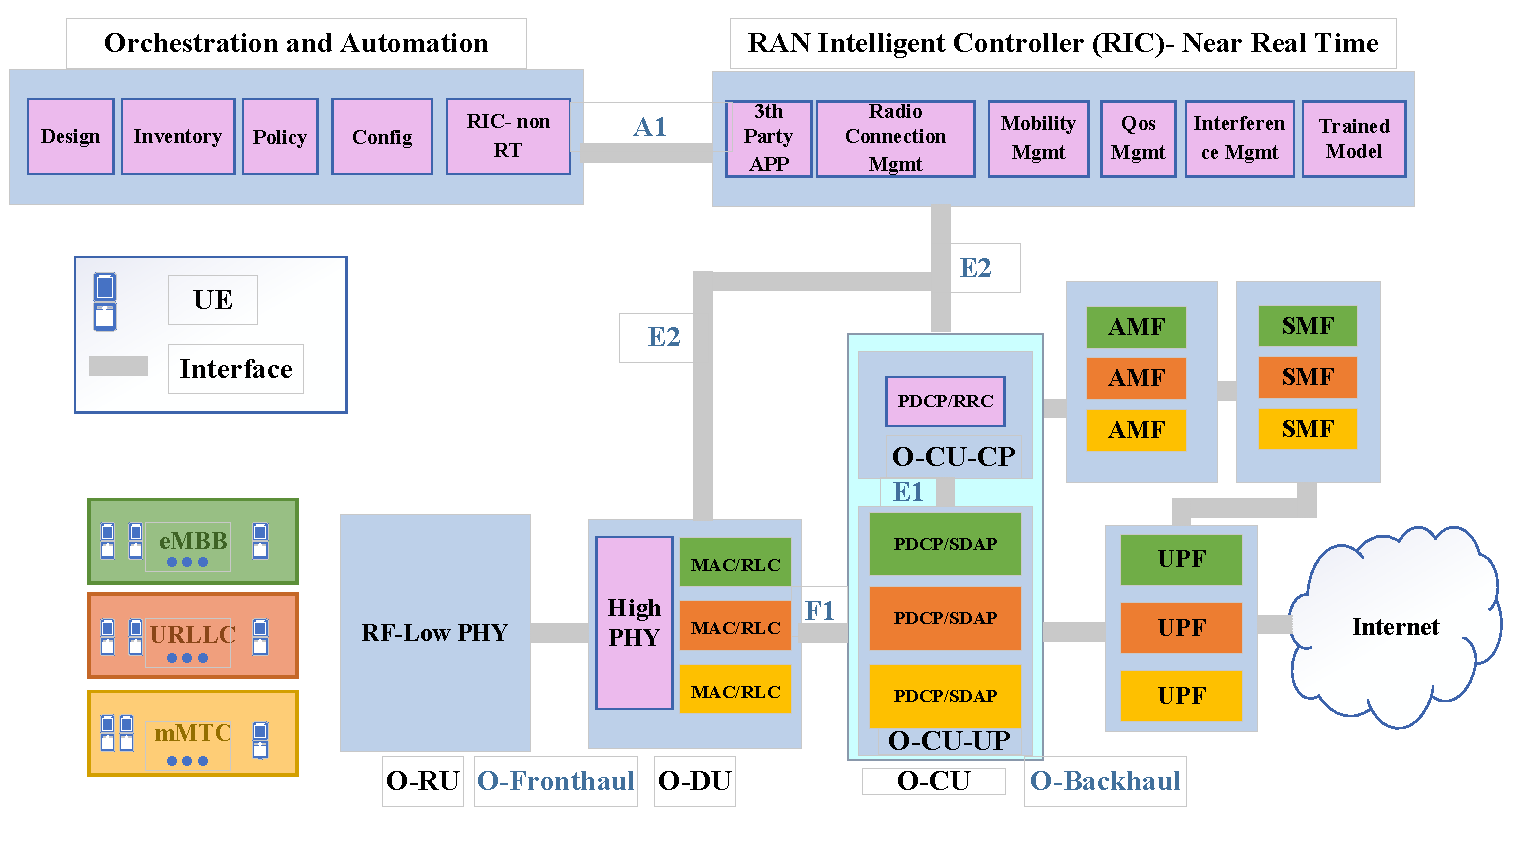
\includegraphics[width=\textwidth]{finalDraw.pdf}
%  \caption{Aggregate Throughput vs. Maximum Interference }
%  \label{fig:13}
%\end{figure}

In Fig. 14, the aggregate throughput is shown versus
the number of UEs for an eMBB service with low interference for the IABV and FA methods in the feasible region.
The minimum data rate for each UE is 1Mb/s/Hz.
The maximum power for each O-RU is 34dBm, and the maximum power for each UE is 30dBm. We assume that the system is not sensitive to fronhaul capacity and end-to-end delay and has enough VNF resources.
By increasing the number of UEs, the aggregate throughput raises.
And we can see that the IABV method is better than the FA method.
%\begin{figure}
%  \centering
%    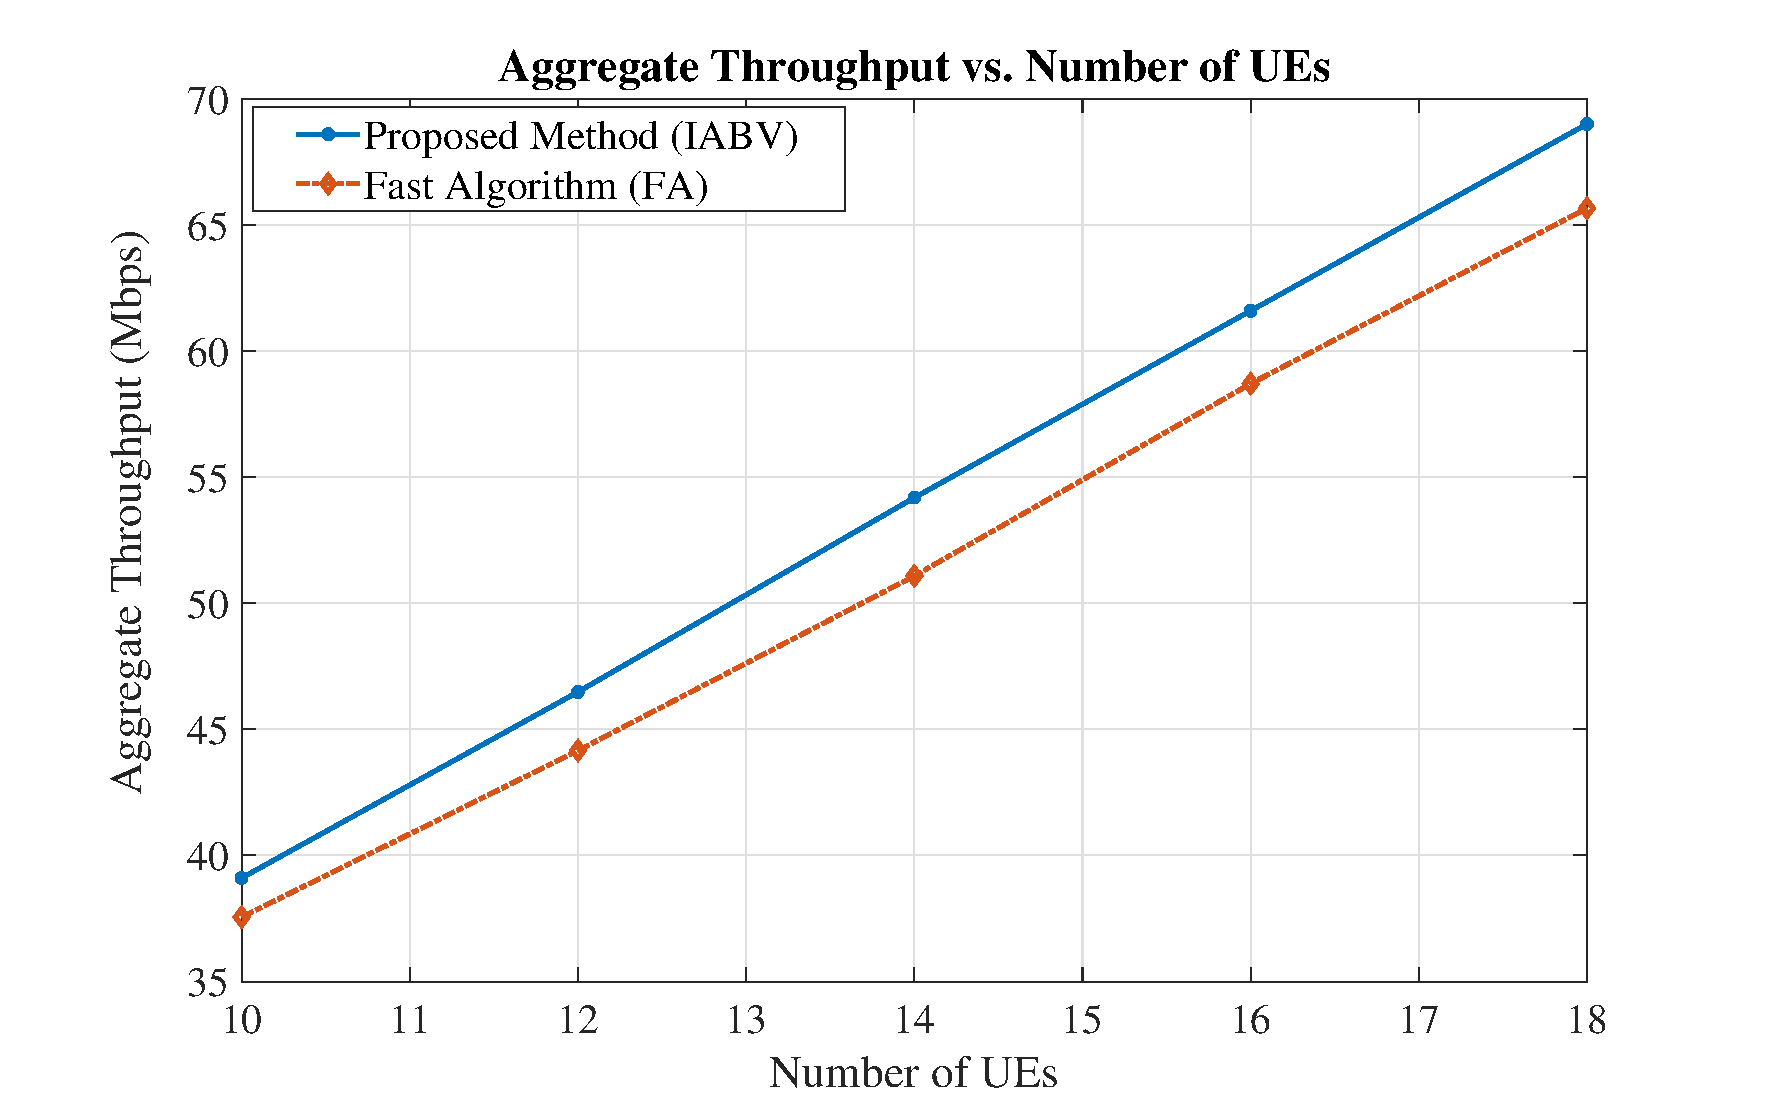
\includegraphics[scale = 0.4]{FA.eps}
%    %\includegraphics[max height=30cm,max width=9.5cm]{Drawing15.eps}
%    %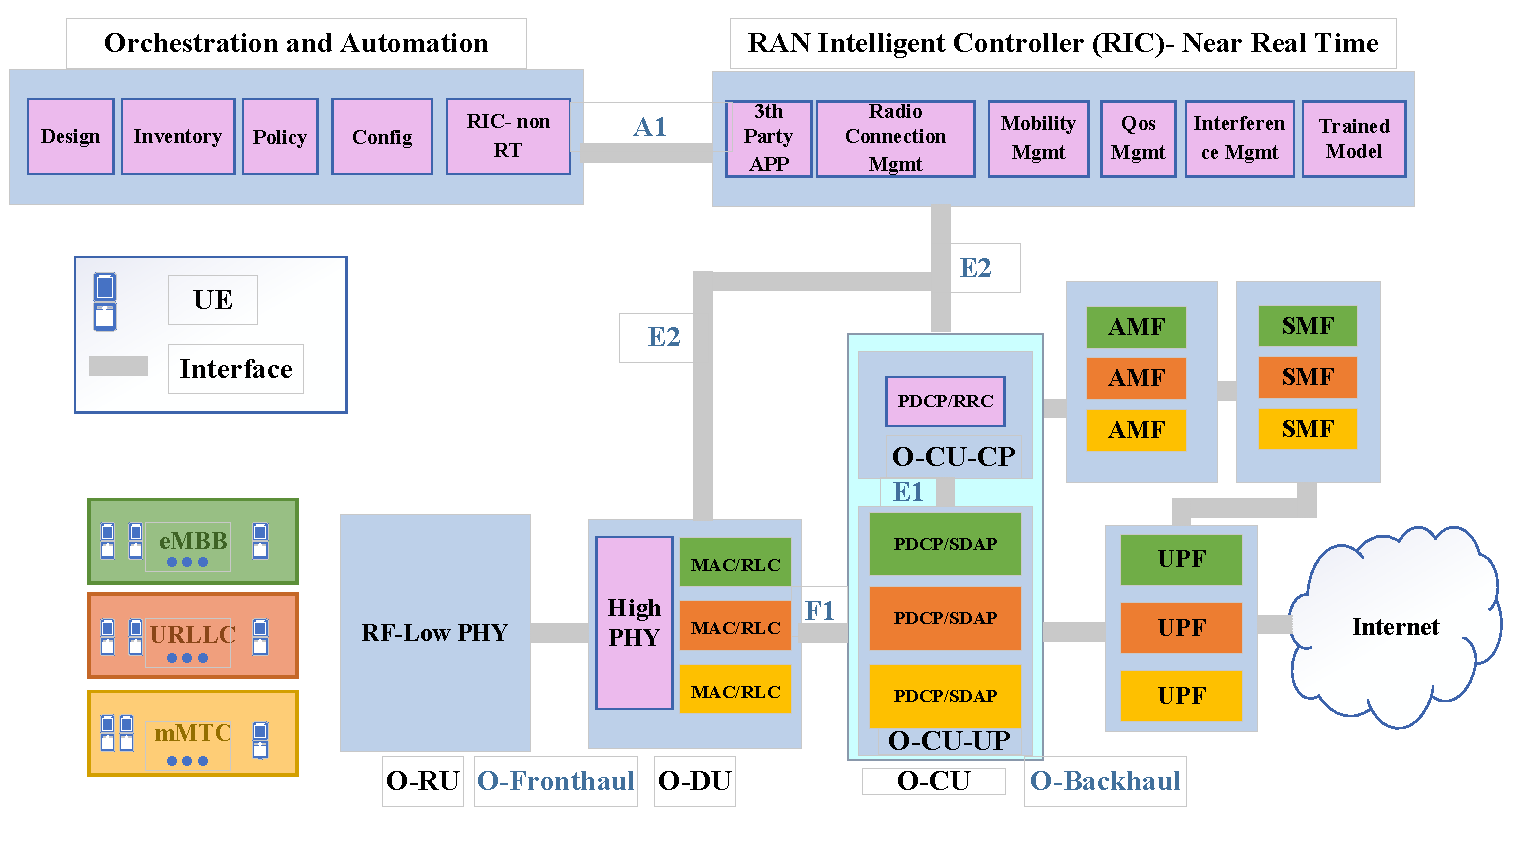
\includegraphics[width=\textwidth]{finalDraw.pdf}
%  \caption{Aggregate Throughput vs. the Number of UEs }
%  \label{fig:14}
%\end{figure}

\textcolor{MidnightBlue}{Table III shows the execution time given a number of UEs for one service for the three methods. We run our simulation on the system with configuration (RAM = 8 GB, CPU = Core i5, SSD Hard Disk). 
 As the number of UEs in the system increases, the execution time increases polynomially for all three algorithms.
Since the baseline scheme is a simpler algorithm, with random PRB allocation and O-RU association based on distance, the execution time is less than the two other algorithms. Power and PRB are allocated in the DR scheme, but O-RUs are associated based on distance. Therefore the execution time is less than the proposed algorithm.}
\begin{table}%[H]
 \caption {Execution Time vs. Number of UEs} 
\begin{center}
 \scalebox{0.75}{
\begin{tabular}{ |l|l|l|l| }
%\hline
%\multicolumn{3}{|c|}{Country List} \\
\hline
\multirow{2}{*}{Number of UEs } &\multicolumn{3}{|c|}{Execution Time (usec)} \\
\cline{2-4}
{} &Proposed method & DR scheme & Baseline scheme \\
\hline
5 & 12.156 &8.9546 &6.6436\\
10 & 19.156   & 12.3112& 8.7870\\
15 &29.140 & 15.4778 &9.5648 \\
20    &44.573 &  21.5342 &14.8334 \\
25 & 67.912  & 30.7926 &21.5510 \\
\hline
\end{tabular}}
\vspace*{-1.6em}
\end{center}
\end{table}
%\begin{figure}[H]
%  \centering
%    \includegraphics[scale = 0.4]{fig/exec.eps}
%    %\includegraphics[max height=30cm,max width=9.5cm]{Drawing15.eps}
%    %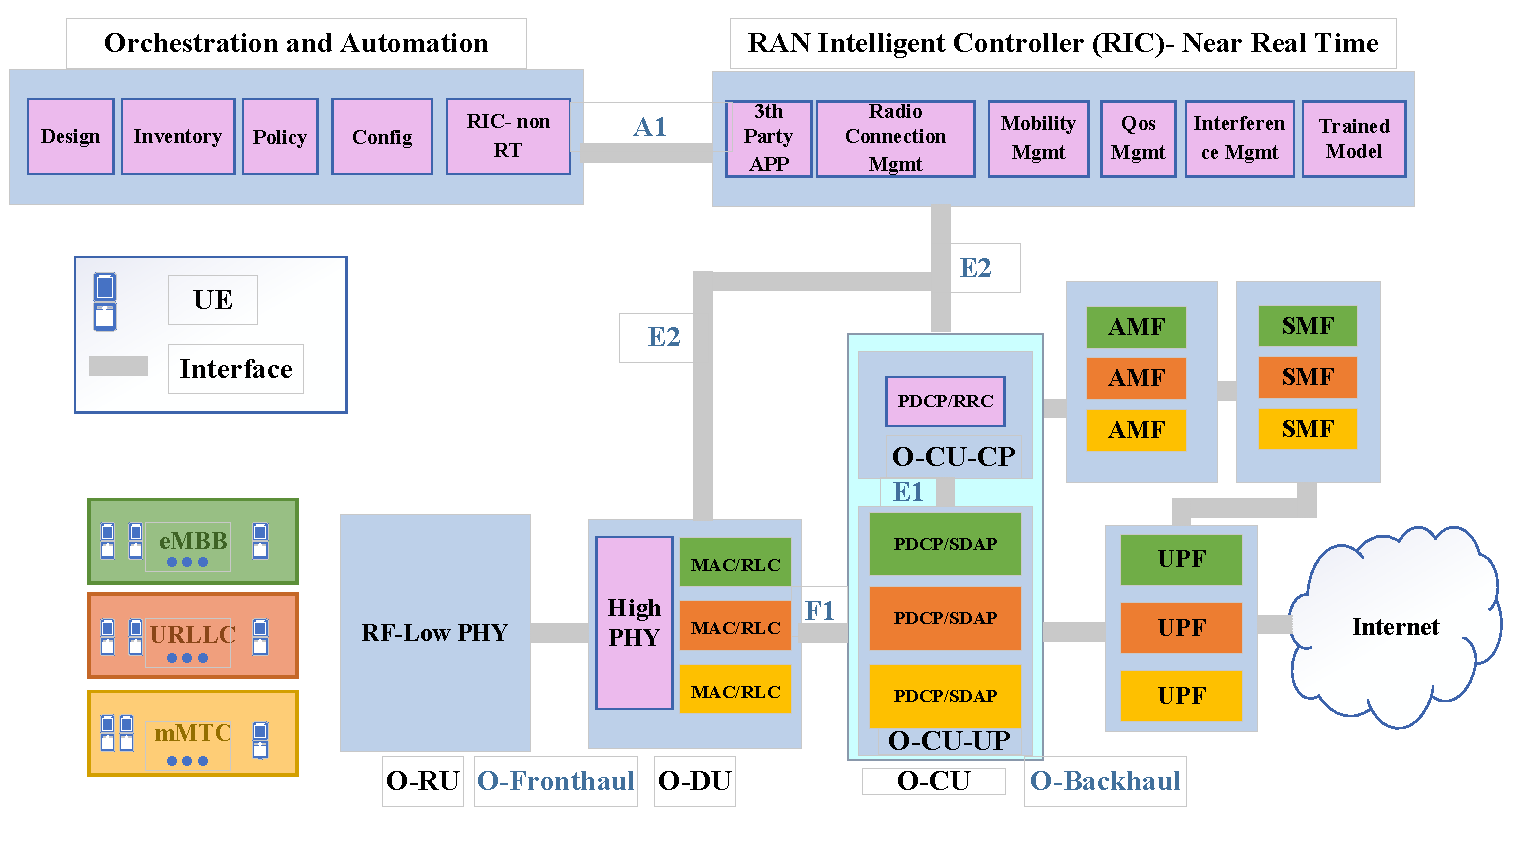
\includegraphics[width=\textwidth]{finalDraw.pdf}
%  %\caption{Mean Total Delay (usec) vs. Number of iterations}
%  \captionsetup{labelformat=empty}
%  \caption{(15) Execution time vs. the number of UEs}
%  \label{fig:2}
%\end{figure}
\vspace*{-1.4em}
\section{Conclusion}\label{conc}
In this paper, we modeled the downlink of the O-RAN system using isolated network slicing for different 5G services, i.e., eMBB, mMTC, and URLLC.
Our goal is to maximize aggregate throughput by activating VNFs in each service, associating RUs, allocating power, and PRBs. The limited fronthaul capacity and the mean delay for each service are considered.
The problem is mixed-integer non-linear programming that is solved by a two-step iterative algorithm.
In the first step, we reformulated the problem to achieve the number of activated VNFs as a function of data rate. Then, we obtained PRB association and power allocation using the Lagrangian method.
In the second step, the O-RU association is carried out.
The performance of our proposed method (i.e., IABV) is compared with the baseline scheme and DR scheme in \cite{lee2018dynamic}.
In addition, the feasible region is discussed, and the FA algorithm is introduced to check the feasibility of the initial values.
Also, we assume distinct scenarios for each service, i.e., eMBB, mMTC, and URLLC, based on their requirement QoS.
Simulation results show that the proposed method (i.e., IABV) achieves $18.6\%$ higher data rate than the baseline scheme.
Moreover, simulation results illustrate more minor delays for the proposed method (IABV) than DR scheme and the baseline scheme.
\vspace*{-1.1em}
\bibliographystyle{IEEEtran}
\bibliography{ref}
%\bibliography{IEEEabrv,conf_short,ref}
\end{document} 
